\documentclass[11pt,a4paper]{article}

\usepackage[margin=1in]{geometry}
\usepackage[T1]{fontenc}
\usepackage[utf8]{inputenc}
\usepackage{lmodern}
\usepackage{amsmath,amssymb,amsfonts}
\usepackage{booktabs,longtable,tabularx,multirow,array}
\usepackage{pdflscape}
\usepackage{graphicx}
\usepackage{hyperref}
\usepackage{cite}
\usepackage{enumitem}
\usepackage{caption}
\usepackage{subcaption}
\usepackage{microtype}
\usepackage{fancyhdr}
\usepackage{titlesec}
\usepackage{xcolor}
\usepackage{xltabular}

\hypersetup{
    colorlinks=true,
    linkcolor=blue!70!black,
    citecolor=blue!70!black,
    urlcolor=blue!70!black,
    pdftitle={Phase 2 Extended Literature Review and Research Methodology},
    pdfauthor={Saif Shahzad and Shahoud Shahid}
}

\pagestyle{fancy}
\fancyhf{}
\fancyhead[L]{\small Phase 2: Extended Literature Review \& Research Methodology}
\fancyhead[R]{\small Computer Networks}
\fancyfoot[C]{\thepage}
\renewcommand{\headrulewidth}{0.4pt}
\setlength{\headheight}{14pt}

\titleformat{\section}{\large\bfseries}{\thesection}{1em}{}
\titleformat{\subsection}{\normalsize\bfseries}{\thesubsection}{1em}{}
\titleformat{\subsubsection}{\small\bfseries}{\thesubsubsection}{1em}{}

% Table helpers (added in the revision; do not change the visual style)
\newcolumntype{L}[1]{>{\raggedright\arraybackslash}p{#1}}
\renewcommand{\arraystretch}{1.15}
\urlstyle{same}

\begin{document}

% -------------------------------------------------------------
% Title Page
% -------------------------------------------------------------
\begin{titlepage}
    \centering
    \vspace*{1.5cm}

    {\huge\bfseries Computer Networks Research Project\par}
    \vspace{0.8cm}
    {\LARGE\bfseries Phase 2: Extended Literature Review and\\Research Methodology\par}
    \vspace{1.2cm}

    \rule{\linewidth}{1.2pt}\\[0.4cm]
    {\Large\bfseries Directed Multigraph Graph Neural Networks for Real-Time Anti-Money Laundering on Cryptocurrency Transaction Networks\par}
    \rule{\linewidth}{1.2pt}\\[1.5cm]

    \begin{minipage}{0.48\textwidth}
        \begin{flushleft} \large
            \textbf{Submitted by:}\\[0.2cm]
            Saif Shahzad (23I-2634)\\
            Shahoud Shahid (23I-2515)\\[0.4cm]
            \textbf{Program:} BS Data Science\\
            \textbf{Department:} Artificial Intelligence and Data Science
        \end{flushleft}
    \end{minipage}
    \hfill
    \begin{minipage}{0.48\textwidth}
        \begin{flushright} \large
            \textbf{Course:} Computer Networks\\
            \textbf{Semester:} 7\\
            \textbf{Academic Year:} 2026\\
            \textbf{Submission Date:} October 20, 2026\\
            \textbf{Revision 2:} October 25, 2026
        \end{flushright}
    \end{minipage}

    \vfill
    {\large National University of Computer and Emerging Sciences (FAST-NUCES)\par}
    \vspace*{1cm}
\end{titlepage}

\newpage
\tableofcontents
\newpage
\listoffigures
\listoftables
\newpage

% =============================================================
\section{Introduction and Project Context}
\label{sec:intro}

Public blockchains such as Bitcoin and Ethereum settle value transfers between pseudonymous accounts without intermediaries. The same properties that make them attractive (global reach, irreversibility and permissionless participation) also make them attractive for laundering criminal proceeds. Chainalysis estimates that illicit cryptocurrency addresses received \emph{at least} US\$154 billion in 2025, which the company explicitly describes as a lower-bound estimate \cite{chainalysis2026crime}.

Rule-based anti-money laundering (AML) monitoring relies largely on per-account thresholds and static heuristics (aggregate inflow, velocity, watch-lists). Laundering, however, is a \emph{relational and temporal} activity that is deliberately spread across many accounts and many transfers. Typical patterns include:
\begin{enumerate}[leftmargin=*]
    \item \textbf{Fan-out / fan-in and scatter--gather:} funds are split across many intermediary accounts and later re-aggregated, often through many small parallel transfers. These typologies (together with cycles, bipartite, stack and random patterns) are exactly those simulated in the IBM synthetic AML benchmark \cite{altman2023ibmaml}.
    \item \textbf{Peeling chains (UTXO chains):} a large unspent output is repeatedly split, sending a small amount onward and returning change, producing long, directed chains of transactions.
    \item \textbf{Bursty layering:} many transfers between the same pair of accounts within a short interval, which a static, per-pair summary (``total amount sent from $u$ to $v$'') hides.
\end{enumerate}

Graph Neural Networks (GNNs) \cite{kipf2017gcn,hamilton2017sage,velickovic2018gat} learn from such relational structure. When applied to blockchains, nodes are accounts (or transactions) and edges are timestamped, valued transfers. Our extended review of nine 2025--2026 studies (Sections~\ref{sec:individual_analyses}--\ref{sec:comparison_table}) and of the closest earlier work (Section~\ref{sec:prior_work}) shows three recurring, evidence-backed limitations:
\begin{enumerate}[leftmargin=*]
    \item \textbf{Lossy multigraph collapse.} Several recent pipelines merge all transfers between an account pair into a single edge before learning: Tian and Zhang sum the amounts of parallel edges \cite{tian2025kar}, Al-E'mari et al.\ remove duplicate transaction edges \cite{alemari2026explainable}, and the IJCAI-26 TAML system defines one edge per account pair whose features aggregate all transactions within a time span \cite{rico2026taml}.
    \item \textbf{Batch or snapshot processing.} Strong recent detectors are trained and evaluated on static graphs or discrete snapshots; their authors list streaming, incremental updating and temporal memory as future work \cite{lin2026chronowave,jia2025lmae4eth}. No reviewed AML study quantifies how detection quality depends on \emph{how frequently} the model's view of the network is updated.
    \item \textbf{Evaluation protocols that hinder comparison.} Random or stratified node splits \cite{jia2025lmae4eth,kasula2025ajk,alemari2026explainable}, undocumented splits and baselines copied from other papers \cite{li2025tfgat}, and balanced re-sampling \cite{tian2025kar} make reported numbers difficult to compare and can overstate deployable performance.
\end{enumerate}

These limitations must be read against important earlier work. Some of it already handles directed multigraphs offline (Multi-GNN \cite{egressy2024multigraph}, DIAM \cite{ding2024diam}, MEGA-GNN \cite{bilgi2026mega}) or streams hand-engineered subgraph features in real time (Graph Feature Preprocessor \cite{blanusa2024gfp}). Other work studies, in generic temporal-graph settings, the staleness that batching causes in memory-based models (PRES \cite{su2024pres}, BADGNN \cite{zhou2025badgnn}, AnchorRM \cite{anchorrm2026}, StreamTGN \cite{streamtgn2026}). Our contribution is therefore deliberately narrow and testable. Its primary part is a \emph{measurement}: how much detection quality and timeliness a learned AML detector loses when the transaction stream is processed in coarser, block-like update units, whether that loss falls disproportionately on illicit transfers, and what finer updates cost in latency and throughput. Its secondary part is a \emph{method}: \textbf{Directed Multigraph Temporal Graph Neural Networks (DMT-GNN)}, a continuous-time, memory-based GNN that keeps every transfer as a separate directed event and aggregates parallel transfers per counterparty, together with a lightweight \emph{intra-block context} that gives each transfer exact statistics of the earlier transfers of the same accounts inside the current update unit.

\paragraph{Revision note (Revision 2, aligned with Phase 3).} This revision keeps the literature review (Sections~\ref{sec:selection}--\ref{sec:comparison_table}) and the nine paper analyses unchanged. It (i) adds recent work that bears directly on our claims (FraudGT's reported results, SALT-GNN, and the batch-staleness literature; Section~\ref{sec:prior_work}); (ii) makes the freshness question the primary research question and adds the intra-block context as a tested mitigation (Section~\ref{sec:refined_gap}); (iii) aligns preprocessing with Multi-GNN's released code, reduces seeds to three, drops MEGA-GNN as a baseline and makes the Ethereum dataset conditional (Section~\ref{sec:methodology}); and (iv) replaces the twelve-week plan with a 21-day, compute-constrained Phase 3 plan (Section~\ref{sec:execution_plan}).

\paragraph{Why this is a Computer Networks project.} A blockchain is a peer-to-peer network that delivers transactions to observers as a stream whose granularity is set by the protocol (blocks), and an AML detector is a stream-processing service attached to that network. Our evaluation therefore treats detection as a networked service: we replay transaction streams under different arrival granularities (per event, micro-batch, block-like time buckets) and offered loads. We then measure end-to-end latency percentiles, sustained throughput, queueing behaviour, memory growth and \emph{detection delay}, alongside classification quality (Steps 7--8, Section~\ref{sec:methodology}). This systems-level question, namely how much detection quality is lost when the model's view of the network is refreshed less often and how much latency is paid to refresh it more often, is the part of the work most directly grounded in computer networking.

% =============================================================
\section{Connection to the Phase 1 Literature Review}
\label{sec:phase1_connection}

In Phase 1 we established the topic \textit{``Directed Multigraph GNNs for Real-Time AML on Cryptocurrency Transaction Networks''} and critically analysed three 2026 works. These three papers are \emph{not} counted towards the Phase 2 quota.
\begin{enumerate}[leftmargin=*]
    \item \textbf{TcfDyG \cite{li2026tcfdyg}} (\textit{Blockchain: Research and Applications}, 2026, Art.\ no.\ 100553): a continuous-time dynamic GNN with time-aware neighbour sampling, multi-channel feature encoding and MLP-Mixer channel fusion, evaluated mainly on temporal \emph{link prediction} (including Bitcoin-Alpha, Bitcoin-OTC and Ethereum phishing interaction graphs). Limitations noted in Phase 1: link-prediction framing rather than transaction-level AML decisions, local sampling, and no streaming latency analysis.
    \item \textbf{ETX2Vec \cite{lu2026etx2vec}} (\textit{Scientific Reports}, 16, Art.\ no.\ 16743, 2026): temporal, amount-biased random walks with Skip-Gram embeddings on an Ethereum transaction multigraph that keeps timestamps and amounts on edges. Limitations: no GNN backbone, transductive and offline, one-hop subgraphs.
    \item \textbf{FG-EGCN \cite{han2026fgegcn}} (\textit{Scientific Reports}, 16, Art.\ no.\ 22352, 2026): an EvolveGCN-H temporal encoder with a residual feature branch, node-wise feature gating and focal loss on Elliptic. Limitations: discrete snapshots, no edge-level multiplicity, online updating left to future work.
\end{enumerate}

\subsection{Phase 1 Core Research Gaps}
The Phase 1 synthesis identified four gaps:
\begin{itemize}[leftmargin=*]
    \item \textbf{Gap 1 (Structural):} no integrated directed-multigraph temporal GNN that preserves parallel transfers, fund-flow direction and continuous time.
    \item \textbf{Gap 2 (Operational):} no end-to-end streaming evaluation (latency, throughput, online memory updates).
    \item \textbf{Gap 3 (Generalization):} reliance on single or synthetic benchmarks without cross-domain validation.
    \item \textbf{Gap 4 (Forensic):} insufficient explanations for investigators.
\end{itemize}

\subsection{How Phase 2 Refines the Phase 1 Gaps}
Phase 2 preserves the research topic, motivation and direction of Phase 1. The extended literature (Sections~\ref{sec:individual_analyses}--\ref{sec:research_gaps}) changes \emph{how} each gap is framed, as summarized in Table~\ref{tab:gap_evolution}. The main change is that the closest earlier work shows that ``a GNN that handles directed multigraphs'' is no longer an open problem in the \emph{offline} setting. The defensible gap is the behaviour of learned AML detectors under realistic streaming conditions (how detection quality and delay depend on update freshness, and at what latency cost), with multigraph-aware aggregation inside continuous-time memory as a secondary, controlled question.

\begin{table}[htbp]
\centering
\small
\caption{Evolution of the Phase 1 Research Gaps into the Refined Phase 2 Gaps}
\label{tab:gap_evolution}
\begin{tabularx}{\textwidth}{L{2.9cm} X L{3.0cm}}
\toprule
\textbf{Phase 1 gap} & \textbf{What the Phase 2 evidence shows} & \textbf{Phase 2 status} \\
\midrule
Gap 1 (Structural) & Offline multigraph GNNs exist \cite{egressy2024multigraph,ding2024diam,bilgi2026mega}, but recent 2025--2026 AML pipelines still collapse parallel transfers \cite{tian2025kar,alemari2026explainable,rico2026taml}, and no reviewed work combines multi-edge aggregation with continuous-time memory. & Refined into \textbf{G1} (Section~\ref{sec:research_gaps}). \\
\midrule
Gap 2 (Operational) & Per-batch latency is sometimes reported \cite{lin2026chronowave,kasula2025ajk}, and high offline throughput exists \cite{egressy2024multigraph}; batch staleness is studied for generic temporal graphs \cite{su2024pres,anchorrm2026,streamtgn2026}. What is missing for AML is the quality--freshness--latency trade-off, including detection delay, under realistic arrival. & Refined into \textbf{G2}; the primary research question and the main networking contribution. \\
\midrule
Gap 3 (Generalization) & Random splits, balanced re-sampling and single synthetic benchmarks dominate \cite{jia2025lmae4eth,kasula2025ajk,tian2025kar,rico2026taml}. & Refined into \textbf{G3}: one chronological protocol on D1; the real Ethereum domain (D2) is conditional on compute (Section~\ref{sec:execution_plan}). \\
\midrule
Gap 4 (Forensic) & Post-hoc explanation on static graphs is now evaluated rigorously \cite{alemari2026explainable}, but explaining memory-based temporal models is a separate research problem. & Retained as \textbf{G4}, \emph{explicitly deferred}: qualitative case studies only. \\
\bottomrule
\end{tabularx}
\end{table}

\subsection{Phase 2 Expansion Scope}
Phase 2 analyses \textbf{nine additional papers} published in 2025--2026 in Q1/Q2 journals or CORE A* conferences (Section~\ref{sec:selection}). They are complemented by a positioning study of the closest earlier work, which is outside the 2025--2026 window and therefore not counted (Section~\ref{sec:prior_work}).

% =============================================================
\section{Literature Search, Screening and Verification Protocol}
\label{sec:selection}

\subsection{Search Strategy}
Searches were run in October 2026 across Crossref, IEEE Xplore, SpringerLink/Nature, MDPI, ScienceDirect, the AAAI and IJCAI proceedings, and arXiv (arXiv was used only to locate authors' versions of peer-reviewed papers or closest-prior-work preprints). Query terms combined \{\textit{anti-money laundering, illicit transaction, phishing, fraud}\} with \{\textit{graph neural network, temporal graph, dynamic graph, multigraph}\} and \{\textit{Bitcoin, Ethereum, cryptocurrency, blockchain, financial transaction network}\}.

\subsection{Inclusion Criteria}
A paper was counted towards the Phase 2 quota only if \emph{all} of the following held:
\begin{enumerate}[leftmargin=*]
    \item published (final version of record) in 2025 or 2026;
    \item an original research article (not an editorial, survey, news item or web page);
    \item published in a venue ranked Q1/Q2 (SJR or JCR) or a CORE A*/A conference;
    \item directly relevant to learning on cryptocurrency or financial transaction graphs for illicit-activity detection;
    \item with an identifiable method, dataset and evaluation protocol;
    \item with a full text that we could read in order to verify the details reported in Section~\ref{sec:individual_analyses}.
\end{enumerate}

\subsection{Verification Procedure}
For each paper we (i) verified title, authors, venue, volume/pages or article number, year and DOI against Crossref metadata and the publisher's landing page; (ii) read the full text (publisher version, or the authors' version where the publisher page was not machine-readable) and checked every number reported in this document against it; and (iii) checked the venue ranking against the CORE portal (conferences) or SJR/JCR-derived listings (journals). The SCImago portal itself blocked automated access during this review. Journal quartiles were therefore taken from publisher bibliometric pages and secondary SJR/JCR mirrors, and are labelled as such in Appendix~\ref{app:verification}. Where a detail could not be verified, it is either omitted or explicitly marked as ``not reported in the version examined''.

\subsection{Included Papers}
Table~\ref{tab:eligibility_audit} lists the nine included papers.

\begin{table}[htbp]
\centering
\scriptsize
\caption{Eligibility Audit of the Nine Phase 2 Papers (all metadata verified against Crossref)}
\label{tab:eligibility_audit}
\begin{tabularx}{\textwidth}{L{0.55cm} L{3.3cm} L{0.6cm} L{2.6cm} L{2.2cm} X}
\toprule
\textbf{\#} & \textbf{First author / short title} & \textbf{Year} & \textbf{Venue (publisher)} & \textbf{Ranking} & \textbf{Relevance to this project} \\
\midrule
P1 & X.~Yang --- GeneralDyG \cite{yang2025generaldyg} & 2025 & Proc.\ AAAI-25 (AAAI) & CORE2023 A* & Event-level temporal ego-graph anomaly detection; evaluated on Bitcoin-Alpha/OTC trust networks. \\
P2 & Z.~Tian --- KAR \cite{tian2025kar} & 2025 & Electronics (MDPI) & SJR Q2 (Comp.\ Netw.\ \& Comm.)$^{\dagger}$ & Continual GNN learning on the Ethereum phishing multigraph; explicitly merges parallel edges. \\
P3 & S.~Ferretti --- AML GNN benchmark \cite{ferretti2025aml} & 2025 & IEEE Access (IEEE) & SJR Q1$^{\dagger}$ (SJR 2024 = 0.849) & Controlled comparison of GNN families and feature sets for Bitcoin AML (Elliptic). \\
P4 & M.~Li --- TFGAT \cite{li2025tfgat} & 2025 & Scientific Reports (Springer Nature) & JCR Q1$^{\dagger}$ (Multidiscipl.) & Global--local attention and pseudo-labelling for Bitcoin AML. \\
P5 & V.~K.~Kasula --- AJKGS-ABCM \cite{kasula2025ajk} & 2025 & Discover Artificial Intelligence (Springer Nature) & SJR Q1$^{\dagger}$ (SJR 2024 = 0.876) & Multi-class Ethereum address classification with attention and jumping knowledge; reports latency. \\
P6 & Y.~Jia --- LMAE4Eth \cite{jia2025lmae4eth} & 2025 & IEEE Trans.\ Inf.\ Forensics Security (IEEE) & SJR Q1$^{\dagger}$ (Comp.\ Netw.\ \& Comm.) & Transaction-semantics language model + masked graph autoencoder for Ethereum fraud; three real datasets. \\
P7 & Z.~Lin --- ChronoWave-GNN \cite{lin2026chronowave} & 2026 & Scientific Reports (Springer Nature) & JCR Q1$^{\dagger}$ (Multidiscipl.) & Temporal graph transformer for Bitcoin AML with latency profiling; batch-mode. \\
P8 & S.~Al-E'mari --- Explainable GNNs \cite{alemari2026explainable} & 2026 & Future Internet (MDPI) & SJR Q2 (Comp.\ Netw.\ \& Comm.)$^{\dagger}$ & Multi-class Ethereum fraud with statistical testing and quantitative explanations. \\
P9 & R.~Rico --- TAML \cite{rico2026taml} & 2026 & Proc.\ IJCAI-26 (IJCAI) & CORE2023 A* & Joint AML classification and sub-network discovery; evaluated on IBM AML, SAML-D, Elliptic++. \\
\bottomrule
\end{tabularx}
\par\smallskip
{\scriptsize $^{\dagger}$Quartile taken from a publisher bibliometrics page or a secondary SJR/JCR listing (the SCImago portal blocked automated access); see Appendix~\ref{app:verification}.\par}
\end{table}

\subsection{Screened but Excluded Candidates}
Transparency about exclusions is part of a defensible review. Table~\ref{tab:excluded} lists candidates that were screened and \emph{not} counted, with reasons. Three of them appeared in our earlier Phase 2 draft and were removed from the quota after verification.

\begin{table}[htbp]
\centering
\scriptsize
\caption{Screened Candidates Excluded from the Phase 2 Quota}
\label{tab:excluded}
\begin{tabularx}{\textwidth}{L{4.0cm} L{2.6cm} X}
\toprule
\textbf{Candidate} & \textbf{Venue / year} & \textbf{Reason for exclusion (and how it is used instead)} \\
\midrule
Chen et al., MDST-GNN \cite{chen2025mdst} & Adv.\ Intell.\ Syst., 2025 & Metadata verified, but the full text could not be accessed for verification (publisher bot-protection page); only the abstract could be checked. Excluded so that no unverifiable numbers enter the review. \\
\midrule
Zhou \& Abbas, unsupervised dynamic GNN \cite{zhou2025unsup} & IEEE Access, 2025 & Evaluated only on non-financial graphs (communication and protein networks) for link prediction; insufficient relevance. \\
\midrule
Asiri \& Somasundaram, GCN fraud detection \cite{asiri2025gcn} & Sci.\ Rep., 2025 & Full text (PubMed Central) contains integrity anomalies: metric definitions refer to ``skin cancer'', the training table reports 0.9856 training accuracy against 0.168 validation accuracy, the text calls an AUC of 0.9444 ``perfect'', and it states that ``random feature vectors are assigned to generate synthetic features''. Cited only as a cautionary example in Section~\ref{sec:thematic_review}. \\
\midrule
Li et al., TGDAMFormer (Appl.\ Intell., 2026) & Applied Intelligence, 2026 & Directly relevant (Elliptic++), but subscription-only; the method could not be verified beyond the abstract. \\
\midrule
Egressy et al.\ \cite{egressy2024multigraph}; Ding et al.\ \cite{ding2024diam}; Blanu\v{s}a et al.\ \cite{blanusa2024gfp}; Lin et al.\ \cite{lin2024fraudgt} & AAAI-24; CIKM-24; ICAIF-24; ICAIF-24 & Highly relevant but published in 2024 (outside the window); analysed as closest prior work in Section~\ref{sec:prior_work}. \\
\midrule
Bilgi \& Atasu, MEGA-GNN \cite{bilgi2026mega} & TMLR (accepted, 2026) & Highly relevant, but a Q1/Q2 ranking for TMLR could not be verified; analysed as closest prior work. \\
\midrule
TeMP-TraG \cite{gounoue2025tempt}; Amatriciana \cite{digennaro2025amatriciana} & arXiv preprints & Not verifiable as peer-reviewed 2025--2026 Q1/Q2 publications; used as related work only. \\
\bottomrule
\end{tabularx}
\end{table}

\section{Detailed Individual Paper Analyses}
\label{sec:individual_analyses}

Each of the nine included papers is analysed under the fifteen headings (A--O) used throughout this review. All numbers below were checked against the full text examined (Appendix~\ref{app:verification}). Statements under headings L--O are our own assessment unless they are explicitly attributed to the authors. Details that the paper does not report are stated as such rather than inferred.

% =========================================================================
% Paper 1: GeneralDyG (Yang et al., AAAI 2025)
% =========================================================================
\subsection{Paper 1: GeneralDyG --- A Generalizable Anomaly Detection Method in Dynamic Graphs}
\label{sec:p1_generaldyg}

\subsubsection*{A. Bibliographic Information and Eligibility}
\begin{itemize}[leftmargin=*]
    \item \textbf{Full Title:} A Generalizable Anomaly Detection Method in Dynamic Graphs
    \item \textbf{Authors:} Xiao Yang, Xuejiao Zhao, and Zhiqi Shen
    \item \textbf{Publication Year:} 2025 (published April 11, 2025)
    \item \textbf{Venue:} \textit{Proceedings of the AAAI Conference on Artificial Intelligence} (AAAI-25), Vol.~39, No.~20, pp.~22001--22009
    \item \textbf{Publisher:} Association for the Advancement of Artificial Intelligence (AAAI)
    \item \textbf{DOI / Source URL:} \href{https://doi.org/10.1609/aaai.v39i20.35508}{10.1609/aaai.v39i20.35508}; open access: \url{https://ojs.aaai.org/index.php/AAAI/article/view/35508}
    \item \textbf{Ranking / Quartile:} CORE2023 \textbf{A*} (verified on the ICORE conference portal).
    \item \textbf{Relevance to This Project:} Event-level anomaly detection on continuous-time dynamic graphs, evaluated on two Bitcoin trading trust networks. Relevant to how temporal neighbourhoods around an event can be sampled; it does not address AML labels or transaction multigraphs directly.
    \item \textbf{Eligibility Decision:} \textbf{Eligible.} Original research published in 2025 at a CORE A* venue; full text examined (authors' version, arXiv:2412.16447).
\end{itemize}

\subsubsection*{B. Research Problem and Motivation}
The authors argue that existing dynamic-graph anomaly detectors generalise poorly across domains because of three challenges: \textit{data diversity} (graphs differ in structure and feature semantics), \textit{dynamic feature capture} (structural and temporal changes are entangled), and \textit{computational cost}. They aim for one detector that works for both node-level and edge-level anomalies across different dynamic graphs.

\subsubsection*{C. Research Objectives and Contributions}
\begin{enumerate}[leftmargin=*]
    \item \textit{Temporal ego-graph sampling:} for each event, a temporal $k$-hop ego-graph is extracted around it, with hierarchical tokens marking the hop levels of the ego-graph.
    \item \textit{TensGNN:} a GNN extractor that alternates node-feature and edge-feature propagation layers (the final layer is a node layer for node-level tasks and an edge layer for edge-level tasks), embedding nodes, edges and topology into the feature space.
    \item \textit{Temporal-aware Transformer:} the topological structure information of the ego-graph is overlaid on the Query and Key, while the original event features are retained.
\end{enumerate}

\subsubsection*{D. Related Work and Theoretical Foundation}
The paper builds on continuous-time dynamic graph (CTDG) learning (e.g., TGAT \cite{xu2020tgat}, TGN \cite{rossi2020tgn}) and on dynamic-graph anomaly detectors such as TADDY, StrGNN, SAD and SLADE, and node-level detectors such as GDN and FuSAGNet. It positions ego-graph sampling as a way to keep computation local while still capturing temporal context.

\subsubsection*{E. Dataset and Data Collection}
\begin{itemize}[leftmargin=*]
    \item \textbf{Edge level:} Bitcoin-Alpha and Bitcoin-OTC, trust networks of Bitcoin users trading on the btc-alpha.com and bitcoin-otc.com platforms. Following the TADDY protocol, anomalies are injected into the test set at 1\%, 5\% and 10\%.
    \item \textbf{Node level:} SWaT and WADI (water-treatment sensor graphs), used as in GDN.
\end{itemize}

\subsubsection*{F. Preprocessing and Feature Engineering}
Each event is represented by its temporal $k$-hop ego-graph; node, edge and topological structure information are mapped into the feature space, and hierarchical tokens encode the hop level of each element. The paper does not use transaction amounts or AML-specific features.

\subsubsection*{G. Model Architecture and Technical Methodology}
The ego-graph sequence is encoded by TensGNN (alternating node and edge propagation) and then by a Transformer whose attention is conditioned on the ego-graph topology (structure injected into Query and Key; original features kept in the Value path). Anomaly scores are produced for the target edge or node.

\subsubsection*{H. Experimental Setup}
GeneralDyG is compared with 20 baselines spanning graph embeddings (node2vec, DeepWalk), dynamic GNNs (TGAT, TGN), dynamic-graph anomaly detectors (AddGraph, StrGNN, TADDY, SAD, SLADE) and node-level detectors (GDN, BTAD, MST-GAT, FuSAGNet, MTAD-GAT and others). Implementation hyperparameters and hardware are not reported in the version examined and are therefore not stated here.

\subsubsection*{I. Evaluation Metrics}
Edge level: ROC-AUC and Average Precision (AP). Node level: F1.

\subsubsection*{J. Results and Quantitative Interpretation}
\begin{itemize}[leftmargin=*]
    \item \textbf{Bitcoin-Alpha (AUC / AP, \%):} 94.01 / 24.00 (1\% anomalies); 95.41 / 24.02 (5\%); 96.28 / 26.73 (10\%).
    \item \textbf{Bitcoin-OTC (AUC / AP, \%):} 94.66 / 27.89 (1\%); 94.86 / 29.97 (5\%); 95.59 / 27.13 (10\%).
    \item \textbf{Node level (F1, \%):} SWaT 85.19 (second best: FuSAGNet 83.69); WADI 60.43 (slightly below FuSAGNet, 60.70).
\end{itemize}
Note that AP remains below 0.30 even when AUC exceeds 0.94, a reminder that ROC-AUC alone overstates performance on rare anomalies \cite{saito2015prroc}.

\subsubsection*{K. Ablation Studies and Component Analysis}
Bitcoin-Alpha (10\%) AUC / AP and WADI F1: full model 96.28 / 26.73 and 60.43; without ego-graph sampling 96.01 / 19.33 and 59.45; without TensGNN 92.02 / 22.63 and 55.13; without the Transformer 93.71 / 20.20 and 58.46. Ego-graph sampling contributes most to AP; TensGNN contributes most to AUC and WADI F1.

\subsubsection*{L. Limitations and Weaknesses}
\begin{enumerate}[leftmargin=*]
    \item \textit{Injected anomalies:} the edge-level evaluation uses synthetically injected anomalies, not labelled laundering or fraud.
    \item \textit{No transaction semantics:} the datasets carry no transfer amounts, and repeated interactions between the same pair are not modelled as an explicit multigraph.
    \item \textit{No systems evaluation:} no per-event latency, throughput or streaming evaluation is reported.
\end{enumerate}

\subsubsection*{M. Future Research Directions and Threats to Validity}
The authors propose studying the interpretability of anomaly detection in dynamic graphs and providing stronger theoretical support. The main threat to validity for our purposes is construct validity: injected edge anomalies may not resemble coordinated laundering patterns.

\subsubsection*{N. Relevance to Our Proposed Research}
GeneralDyG shows that sampling a bounded temporal neighbourhood around each event is an effective and computationally contained way to obtain temporal context. This supports the causal event sampler of DMT-GNN (Step 5) and the sampling-budget ablation (A6).

\subsubsection*{O. Paper-Specific Conclusion and Comparative Positioning}
GeneralDyG is a strong, generalisable dynamic-graph anomaly detector, but its evaluation does not involve labelled financial crime, transaction amounts, parallel transfers or streaming latency, which are the dimensions our study targets.

% =========================================================================
% Paper 2: KAR (Tian & Zhang, Electronics 2025)
% =========================================================================
\subsection{Paper 2: Tian \& Zhang --- Continual Graph Learning with Knowledge-Augmented Replay}
\label{sec:p2_kar}

\subsubsection*{A. Bibliographic Information and Eligibility}
\begin{itemize}[leftmargin=*]
    \item \textbf{Full Title:} Continual Graph Learning with Knowledge-Augmented Replay: A Case for Ethereum Phishing Detection
    \item \textbf{Authors:} Zonggui Tian and Du Zhang
    \item \textbf{Publication Year:} 2025 (published August 22, 2025)
    \item \textbf{Venue:} \textit{Electronics} (MDPI), Vol.~14, No.~17, Art.\ no.\ 3345
    \item \textbf{Publisher:} MDPI
    \item \textbf{DOI / Source URL:} \href{https://doi.org/10.3390/electronics14173345}{10.3390/electronics14173345}
    \item \textbf{Ranking / Quartile:} SJR \textbf{Q2}, Computer Networks and Communications (secondary listing; see Appendix~\ref{app:verification}).
    \item \textbf{Relevance to This Project:} Continual learning on the same XBlock Ethereum phishing network we use as D2; explicitly reports collapsing parallel transfers.
    \item \textbf{Eligibility Decision:} \textbf{Eligible.} Peer-reviewed 2025 article in a Q2 venue; full text examined (MDPI open access).
\end{itemize}

\subsubsection*{B. Research Problem and Motivation}
GNNs retrained on new data forget earlier patterns (catastrophic forgetting), while retraining on the full history is expensive. The authors study \emph{sample-incremental} continual graph learning on the evolving Ethereum transaction network and ask how knowledge from later stages can reinforce, rather than overwrite, earlier knowledge.

\subsubsection*{C. Research Objectives and Contributions}
\begin{enumerate}[leftmargin=*]
    \item \textit{Temporal partitioning:} the network is split chronologically into 10 incremental transaction networks (ITNs) with an approximately equal number of phishing accounts each.
    \item \textit{Evolutionary transaction subgraphs:} incremental (ITSG) and accumulative (ATSG) transaction subgraphs describe how an account's transactions evolve; detection is reformulated as classification of first-order subgraphs.
    \item \textit{Knowledge-Augmented Replay (KAR):} a memory buffer stores phishing accounts that reappear in later stages (plus an equal number of reappearing non-phishing accounts) and replays their accumulated subgraphs with inter-stage edges retained.
    \item \textit{An $\epsilon$-$k$ bounded convergence criterion} for continual learning, linking average accuracy to backward transfer.
\end{enumerate}

\subsubsection*{D. Related Work and Theoretical Foundation}
The work draws on continual learning (regularisation methods such as EWC and the topology-aware TWP; distillation such as LwF; and experience replay) and on Ethereum phishing detection with graph embeddings and GNNs. Its key argument is that \emph{inter-stage edges} (connections between the current stage and earlier stages) carry knowledge that most continual-graph-learning methods ignore.

\subsubsection*{E. Dataset and Data Collection}
\begin{itemize}[leftmargin=*]
    \item \textbf{XBlock Ethereum transaction network:} 2,973,489 addresses, 13,551,303 transactions, 1,165 labelled phishing addresses; the largest connected component (2,973,382 addresses; 13,551,214 transactions; 1,157 phishing) is used.
    \item \textbf{Partitioning:} the 1,157 phishing accounts are ordered by first timestamp and allocated to 10 ITNs (116 phishing accounts in each of the first seven, 115 in each of the last three).
    \item \textbf{Class balance:} each stage dataset contains all phishing subgraphs and an \emph{equal number} of randomly selected non-phishing subgraphs.
\end{itemize}

\subsubsection*{F. Preprocessing and Feature Engineering}
\begin{itemize}[leftmargin=*]
    \item \textbf{Parallel-edge collapse:} each snapshot ``is a multigraph''; the authors simplify it ``into a simple graph by merging parallel edges and summing their transaction amounts''.
    \item \textbf{Node features:} number of first-order neighbours, in-degree, out-degree, total degree, in-strength, out-strength and total strength. The paper also lists node labels as an available feature when the task is reformulated as graph classification; any reuse of this design must ensure that the label of the account being classified is never an input.
\end{itemize}

\subsubsection*{G. Model Architecture and Technical Methodology}
Four backbones (GCN, GAT, GATv2, GIN) share a template of two graph convolution layers (50\% dropout), global pooling to a subgraph vector and a linear classifier. KAR, naïve fine-tuning and full retraining differ in how the central-node set and subgraphs are constructed at each stage.

\subsubsection*{H. Experimental Setup}
Within each stage, the balanced dataset is randomly shuffled and split 70/30 into training and test sets. Hidden size $d=32$; maximum epochs $\{100, 300, 500\}$; learning rate $\{0.001, 0.003, 0.005\}$; batch size 32; PyTorch 2.1.2 and PyTorch Geometric on an NVIDIA V100 (16\,GB). EWC, LwF and TWP are compared under a unified protocol.

\subsubsection*{I. Evaluation Metrics}
Average accuracy (ACC) over all stages and backward transfer (BWT), using the standard continual-learning definitions cited by the authors.

\subsubsection*{J. Results and Quantitative Interpretation}
\begin{itemize}[leftmargin=*]
    \item With inter-stage edges retained, KAR and retraining reach or exceed 90\% stage-wise average accuracy (GIN-based variants remain stable or decline slightly); KAR matches retraining while using less memory.
    \item With inter-stage edges removed, naïve fine-tuning and replay stabilise around 50\% and retraining around 60\%, with negative backward transfer indicating forgetting.
    \item With inter-stage edges retained, KAR also outperforms EWC, LwF and TWP on both accuracy and forgetting.
\end{itemize}

\subsubsection*{K. Ablation Studies and Component Analysis}
The central ablation (with versus without inter-stage edges) shows that cross-stage connectivity, not only parameter regularisation, determines whether forgetting occurs on this network.

\subsubsection*{L. Limitations and Weaknesses}
\begin{enumerate}[leftmargin=*]
    \item \textit{Multigraph collapse:} summing parallel transfers removes per-transfer amounts, timing and burst counts.
    \item \textit{Balanced evaluation:} 1:1 class balance and accuracy as the main metric do not reflect precision at the real prevalence ($1{,}165/2{,}973{,}489 \approx 0.04\%$ of addresses).
    \item \textit{Random splits within stages:} the chronological stage structure is respected across stages, but not within each stage.
    \item \textit{First-order subgraphs only.}
\end{enumerate}

\subsubsection*{M. Future Research Directions and Threats to Validity}
The authors propose adapting knowledge augmentation to other continual-learning settings, refining the $\epsilon$-bounded convergence criterion, and applying KAR to broader cryptocurrency anomaly detection, including AML. Threats to validity for our use: the balanced accuracy metric and the label-as-feature design described in heading F.

\subsubsection*{N. Relevance to Our Proposed Research}
KAR is direct evidence for Gap G1 (explicit summing of parallel transfers on the same Ethereum network we use) and shows that temporal connectivity across time periods matters. This motivates retaining state across time (node memory) rather than treating periods independently (Step 5).

\subsubsection*{O. Paper-Specific Conclusion and Comparative Positioning}
KAR demonstrates that preserving cross-period connectivity prevents forgetting on Ethereum, but its simple-graph representation, balanced datasets and stage-level updates leave per-transfer modelling and event-level freshness untested.

% =========================================================================
% Paper 3: Ferretti et al. (IEEE Access 2025)
% =========================================================================
\subsection{Paper 3: Ferretti et al. --- Enhancing AML Frameworks in Cryptocurrency Transactions}
\label{sec:p3_ferretti}

\subsubsection*{A. Bibliographic Information and Eligibility}
\begin{itemize}[leftmargin=*]
    \item \textbf{Full Title:} Enhancing Anti-Money Laundering Frameworks: An Application of Graph Neural Networks in Cryptocurrency Transaction Classification
    \item \textbf{Authors:} Stefano Ferretti, Gabriele D'Angelo, and Vittorio Ghini
    \item \textbf{Publication Year:} 2025 (published March 17, 2025)
    \item \textbf{Venue:} \textit{IEEE Access}, Vol.~13, pp.~50201--50215
    \item \textbf{Publisher:} IEEE
    \item \textbf{DOI / Source URL:} \href{https://doi.org/10.1109/ACCESS.2025.3552240}{10.1109/ACCESS.2025.3552240}
    \item \textbf{Code:} \url{https://github.com/stefano-ferretti/aml-elliptic-gnn}
    \item \textbf{Ranking / Quartile:} SJR \textbf{Q1} (secondary listing); SJR 2024 = 0.849 (IEEE Access bibliometrics page).
    \item \textbf{Relevance to This Project:} Controlled comparison of GNN families and feature sets for Bitcoin AML on Elliptic; isolates the contribution of features versus graph structure.
    \item \textbf{Eligibility Decision:} \textbf{Eligible.} Peer-reviewed 2025 Q1 journal article; full text examined (IEEE Xplore, open access).
\end{itemize}

\subsubsection*{B. Research Problem and Motivation}
Practitioners lack controlled guidance on which GNN architectures and feature sets work best for classifying illicit cryptocurrency transactions. The authors analyse the Elliptic dataset (class imbalance, correlated features) and compare GNN variants under several feature configurations.

\subsubsection*{C. Research Objectives and Contributions}
\begin{enumerate}[leftmargin=*]
    \item Comparison of GCN, GAT, GATv2, GraphSAGE and Chebyshev convolutions.
    \item Three architectural variants per family: a two-layer baseline, a variant with a \emph{final} linear layer (+Lin), and a variant with the linear layer and skip connections (+Lin+Skip).
    \item Three feature configurations: transaction features only (\texttt{tx}), all features (\texttt{tx+agg}), and transaction features plus a reduced set of aggregated features excluding those with very high correlation (\texttt{tx+agg\_red}).
\end{enumerate}

\subsubsection*{D. Related Work and Theoretical Foundation}
Builds on spatial and spectral GNNs \cite{kipf2017gcn,hamilton2017sage,velickovic2018gat} and on the Elliptic benchmark \cite{weber2019elliptic}. Skip connections are motivated as a remedy for over-smoothing in message passing.

\subsubsection*{E. Dataset and Data Collection}
Elliptic: 203,769 transaction nodes and 234,355 directed edges; each node has 167 features, of which the first 94 relate to the transaction itself (e.g., numbers of inputs and outputs) and the rest are aggregated from neighbouring transactions. Timestamps are anonymised time steps (relative ordering only).

\subsubsection*{F. Preprocessing and Feature Engineering}
Feature correlation analysis reveals many aggregated-feature pairs with correlation above 0.8, and several above 0.9; \texttt{tx+agg\_red} excludes aggregated features with ``extraordinary'' correlation to other features. The number of excluded features is not needed for our argument and is not repeated here.

\subsubsection*{G. Model Architecture and Technical Methodology}
Each model has two graph-convolution layers with ReLU and dropout; +Lin adds a final linear layer; +Lin+Skip adds skip connections that preserve information from earlier message-passing rounds before the final linear layer and log-softmax output.

\subsubsection*{H. Experimental Setup}
Adam with an initial learning rate of $9\times10^{-3}$, reduced by a factor of 0.9 when validation loss does not improve for 100 epochs; 64 hidden units (\texttt{tx}) or 110 (\texttt{tx+agg}, \texttt{tx+agg\_red}); up to 13,000 epochs with early-stopping patience of 1,000; 15 repetitions per configuration; one NVIDIA L40 (48\,GB) node. The train/validation/test split protocol is not described in the text examined.

\subsubsection*{I. Evaluation Metrics}
Precision, recall and F1 for the illicit class; an averaged F1 over both classes (described as micro-averaged in the methods and reported as ``M.A.\ F1'' in the results); training time.

\subsubsection*{J. Results and Quantitative Interpretation}
\begin{itemize}[leftmargin=*]
    \item Best configuration: Chebyshev+Lin on \texttt{tx+agg\_red}, with illicit F1 = \textbf{0.906}, precision 0.955, recall 0.863, and averaged F1 0.983.
    \item GATv2 reaches illicit F1 above 0.885 in configurations with aggregated features; GraphSAGE on \texttt{tx+agg} has the highest recall (0.818); GCN-based models perform relatively worse.
    \item \texttt{tx+agg} generally outperforms \texttt{tx}; \texttt{tx+agg\_red} gives ``only marginal improvements'' but the best overall score.
    \item Removing the dataset features and keeping only graph structure (plus structural node metrics) produced ``very poor results''.
\end{itemize}

\subsubsection*{K. Ablation Studies and Component Analysis}
The feature-configuration and architecture-variant grid acts as an ablation: aggregated neighbourhood features help; the final linear layer and skip connections generally help, but not uniformly across architectures (largest gains for GAT).

\subsubsection*{L. Limitations and Weaknesses}
\begin{enumerate}[leftmargin=*]
    \item \textit{Undocumented split protocol}, so leakage across time steps cannot be ruled out from the text.
    \item \textit{Transaction graph without amounts on edges}: Elliptic has no parallel transfers or per-edge values, so multigraph effects cannot be studied.
    \item \textit{Offline evaluation} only; no streaming or latency analysis.
\end{enumerate}

\subsubsection*{M. Future Research Directions and Threats to Validity}
The authors call for more transparent datasets, potentially synthetic transaction networks generated by agent-based models, further study of heterogeneous GNNs (their preliminary heterogeneous results were lower), and methods to explain which nodes, edges and features drive predictions.

\subsubsection*{N. Relevance to Our Proposed Research}
(1) The structure-only failure supports keeping transaction attributes on every event (Step 4). (2) Chebyshev+Lin (0.906) is a reported reference point for Elliptic, not a baseline we reproduce. (3) The authors' call for synthetic agent-based data supports using the IBM simulator data \cite{altman2023ibmaml} as D1 alongside a real chain (D2).

\subsubsection*{O. Paper-Specific Conclusion and Comparative Positioning}
A careful offline benchmark showing that features dominate and that architectural details matter; it does not address multigraph structure, streaming, or a documented temporal protocol.

% =========================================================================
% Paper 4: TFGAT (Li et al., Sci. Rep. 2025)
% =========================================================================
\subsection{Paper 4: TFGAT --- Global-Local Graph Attention with Cyclic Pseudo-Labels}
\label{sec:p4_tfgat}

\subsubsection*{A. Bibliographic Information and Eligibility}
\begin{itemize}[leftmargin=*]
    \item \textbf{Full Title:} Global-local graph attention with cyclic pseudo-labels for bitcoin anti-money laundering detection
    \item \textbf{Authors:} Meng Li, Lu Jia, and XinQiao Su
    \item \textbf{Publication Year:} 2025 (published July 2, 2025)
    \item \textbf{Venue:} \textit{Scientific Reports} (Springer Nature), Vol.~15, Art.\ no.\ 22668
    \item \textbf{Publisher:} Springer Nature
    \item \textbf{DOI / Source URL:} \href{https://doi.org/10.1038/s41598-025-08365-9}{10.1038/s41598-025-08365-9}
    \item \textbf{Ranking / Quartile:} JCR \textbf{Q1}, Multidisciplinary Sciences (secondary listing).
    \item \textbf{Relevance to This Project:} Combines global (Transformer) and local (GAT) attention with semi-supervised pseudo-labelling for Bitcoin AML; reports parameters and training times.
    \item \textbf{Eligibility Decision:} \textbf{Eligible.} Peer-reviewed 2025 Q1 article; full text examined (open access).
\end{itemize}

\subsubsection*{B. Research Problem and Motivation}
The authors identify three challenges: GCNs assign uniform neighbour weights and can be misled by concealed illicit transactions; node-level GCNs fail to extract global information; and labels are expensive, so most transactions are unlabelled (157,205 of Elliptic's 203,769 nodes, about 77\%).

\subsubsection*{C. Research Objectives and Contributions}
\begin{enumerate}[leftmargin=*]
    \item \textbf{TFGAT} with a Global--Local Attention Mechanism: a Transformer encoder extracts global information across transactions, and a GAT layer then attends over local neighbours.
    \item \textbf{DCPLU} (Deep Cyclic Pseudo-Label Updating): a supervised TFGAT generates pseudo-labels for unlabelled nodes; semi-supervised training on true plus pseudo-labels then updates the pseudo-labels cyclically until validation performance converges, without manifold or Euclidean-distance assumptions.
\end{enumerate}

\subsubsection*{D. Related Work and Theoretical Foundation}
Positions itself against supervised GCN-based AML models (GCN, Skip-GCN, EvolveGCN, temporal attention models) and semi-supervised label-propagation methods, whose similarity assumptions the authors argue do not hold for concealed illicit transactions.

\subsubsection*{E. Dataset and Data Collection}
Elliptic: over 200,000 transaction nodes, about 234,000 edges, 49 time steps (about two weeks apart), labels illicit/licit/unknown; ``AF'' denotes all 166 features and ``LF'' the 94 local features in the baseline table.

\subsubsection*{F. Preprocessing and Feature Engineering}
The paper uses the Elliptic features directly; no additional feature engineering or normalisation procedure is described in the text examined. Class imbalance is handled by a weighted cross-entropy loss (weight 1.0 for the legal class; illegal-class weight 10 in the supervised stage and 6 in the semi-supervised stage, chosen by Bayesian optimisation over $[2, 15]$).

\subsubsection*{G. Model Architecture and Technical Methodology}
Two TransformerEncoder layers with 4 heads and $d_{\text{model}}=512$ (selected by Bayesian optimisation from 1--4 layers, 2--8 heads and $\{192, 256, 512, 1024\}$), followed by multi-head GAT attention over neighbours and a two-layer classifier. DCPLU retrains the same architecture with the label set $y_{\text{new}}$ (true labels plus current pseudo-labels), so the parameter count, and hence inference cost, is unchanged.

\subsubsection*{H. Experimental Setup}
1,000 epochs with Adam; $L_2$ weight $5\times10^{-5}$; learning rate reduced by 20\% (supervised) or 10\% (semi-supervised) every 100 iterations; model selection by validation F1. Twenty-one baselines are listed, with results taken from earlier publications (Weber et al., Vassallo et al., Lo et al.) rather than re-run. The train/validation/test split is not described in the text examined. The printed F1 formula (Eq.~20) omits the factor 2.

\subsubsection*{I. Evaluation Metrics}
Illicit-class precision, recall and F1; ROC-AUC.

\subsubsection*{J. Results and Quantitative Interpretation}
\begin{itemize}[leftmargin=*]
    \item TFGAT: precision 0.9813, recall 0.8322, F1 0.9006.
    \item TFGAT + DCPLU: precision \textbf{0.9814}, recall \textbf{0.8390}, F1 \textbf{0.9046}; AUC 0.9187.
    \item Classical label-propagation variants perform markedly worse, which the authors attribute to violated smoothness assumptions.
\end{itemize}

\subsubsection*{K. Ablation Studies and Component Analysis}
Parameters and training time: Transformer only 6.8M, 4.5\,h (the text states 4.7\,h); GAT only 6.6M, 3.2\,h; TFGAT 6.7M, 4.1\,h; TFGAT + DCPLU 6.7M, 5.1\,h. F1: Transformer 0.8603 (0.8674 with DCPLU); GAT 0.8062 (0.8154); TFGAT 0.9006 (0.9046). Removing the Transformer causes the largest drop.

\subsubsection*{L. Limitations and Weaknesses}
\begin{enumerate}[leftmargin=*]
    \item \textit{Undocumented split} and \textit{borrowed baselines} prevent a controlled comparison.
    \item \textit{Global attention over all transactions} scales quadratically with the number of nodes attended to; with 4--5\,h training it is unsuited to frequent updates.
    \item \textit{Static graph}: time steps are not used to model temporal dynamics.
\end{enumerate}

\subsubsection*{M. Future Research Directions and Threats to Validity}
The paper does not state explicit future-work directions in the version examined. The main threats to validity are the unreported split and the non-reproduced baselines.

\subsubsection*{N. Relevance to Our Proposed Research}
TFGAT shows that wider context improves recall, but at a cost that is incompatible with streaming. This motivates bounding the temporal neighbourhood per event ($S_{\text{in}}, S_{\text{out}}$, Step 5) and measuring cost explicitly (Step 8).

\subsubsection*{O. Paper-Specific Conclusion and Comparative Positioning}
High illicit-class F1 on Elliptic with a static, global-attention model; the evaluation protocol and cost leave deployability under streaming unaddressed.

% =========================================================================
% Paper 5: Kasula et al. (Discover AI 2025)
% =========================================================================
\subsection{Paper 5: Kasula et al. --- Blockchain Address Classification Using AJK-GraphSAGE}
\label{sec:p5_kasula}

\subsubsection*{A. Bibliographic Information and Eligibility}
\begin{itemize}[leftmargin=*]
    \item \textbf{Full Title:} Blockchain address classification using graph neural networks for enhanced security and analytics
    \item \textbf{Authors:} Vinay Kumar Kasula, Akhila Reddy Yadulla, Mounica Yenugula, Bhargavi Konda, and Supraja Ayyamgari
    \item \textbf{Publication Year:} 2025 (published October 24, 2025)
    \item \textbf{Venue:} \textit{Discover Artificial Intelligence} (Springer Nature), Vol.~5, Art.\ no.\ 285
    \item \textbf{Publisher:} Springer Nature
    \item \textbf{DOI / Source URL:} \href{https://doi.org/10.1007/s44163-025-00508-1}{10.1007/s44163-025-00508-1}
    \item \textbf{Ranking / Quartile:} SJR \textbf{Q1} (SJR 2024 = 0.876; secondary listing).
    \item \textbf{Relevance to This Project:} Address-level Ethereum classification with attention over layer depths; one of only two reviewed studies that report per-batch inference time.
    \item \textbf{Eligibility Decision:} \textbf{Eligible.} Original 2025 research article in a Q1 journal; full text examined (open access).
\end{itemize}

\subsubsection*{B. Research Problem and Motivation}
Manual-feature classifiers generalise poorly across platforms, and plain neighbourhood aggregation treats all neighbours and all depths equally. The authors aim to classify Ethereum addresses into functional categories (useful for forensics and AML) using adaptive multi-depth graph representations.

\subsubsection*{C. Research Objectives and Contributions}
\begin{enumerate}[leftmargin=*]
    \item \textbf{AJKGS-ABCM:} an attention-guided jumping-knowledge GraphSAGE for address classification under an account-balance model, with attention over neighbours and over layer depths.
    \item A labelled 11-class Ethereum address dataset (22,312 addresses).
    \item Training- and inference-time profiling against GraphSAGE, GATv2 and a Graph Transformer.
\end{enumerate}

\subsubsection*{D. Related Work and Theoretical Foundation}
Builds on GraphSAGE \cite{hamilton2017sage} and Jumping Knowledge networks \cite{xu2018jk}; baselines include KNN on handcrafted features, DeepWalk, Node2Vec, Struc2Vec, I2BGNN, GCN and GraphSAGE.

\subsubsection*{E. Dataset and Data Collection}
\begin{itemize}[leftmargin=*]
    \item \textbf{Labels:} 22,312 addresses compiled from Etherscan, a Kaggle labelled dataset, XLabelCloud and manually validated social-media sources, in 11 classes: Exchange, Mining pool/Mining, Gambling, Token contract, Darknet, Wallet, Scam, ICO (fundraising), Hacker, Mixer and General user. The authors describe the imbalance as moderate (Exchange and General user frequent; Mixer and Darknet rare).
    \item \textbf{Transactions:} 3,437,967 transactions directly involving the labelled addresses, extended with neighbouring interactions to 58,172,811; after removing failed transactions, 59,465,095 valid transactions are used to build node features and the graph.
\end{itemize}

\subsubsection*{F. Preprocessing and Feature Engineering}
Transaction data were collected via the Etherscan API and the Google BigQuery Ethereum dataset; an adjacency structure and account-state node features are built from the transactions. Mini-batches are drawn with stratified sampling to mitigate class imbalance. The exact feature list and normalisation are not restated here.

\subsubsection*{G. Model Architecture and Technical Methodology}
$K$ GraphSAGE layers with neighbour attention produce layer outputs $\mathbf{h}_i^{(1)},\dots,\mathbf{h}_i^{(K)}$. Layer-level attention weights are computed as
\begin{equation}
    \mathbf{A}_i = \operatorname{softmax}\!\left(\mathbf{W}_a \cdot \operatorname{CONCAT}\big(\mathbf{h}_i^{(1)}, \dots, \mathbf{h}_i^{(K)}\big)\right),
\end{equation}
the layer outputs are fused with these weights (jumping knowledge), and a fully connected softmax layer outputs the class probabilities.

\subsubsection*{H. Experimental Setup}
Training ratios of 60\%, 70\% and 80\% with random splits, 20 repetitions each; the 80:20 split is used for the main comparison; embedding dimension 128; timing on an NVIDIA RTX A6000 (48\,GB).

\subsubsection*{I. Evaluation Metrics}
Precision, recall, micro-F1 and macro-F1; training time per epoch and inference time per batch.

\subsubsection*{J. Results and Quantitative Interpretation}
\begin{itemize}[leftmargin=*]
    \item 80:20 split: AJKGS-ABCM precision 0.862, recall 0.852, micro-F1 0.849, macro-F1 \textbf{0.856}; GraphSAGE 0.823, I2BGNN 0.824, GCN 0.807 and KNN 0.648 (macro-F1).
    \item Cost: 14.9\,s per epoch and 20.8\,ms per batch, versus 12.3\,s and 18.4\,ms for GraphSAGE (GATv2: 16.7\,s and 24.6\,ms; Graph Transformer: 21.5\,s and 32.1\,ms).
\end{itemize}

\subsubsection*{K. Ablation Studies and Component Analysis}
The comparison with plain GraphSAGE isolates the attention and jumping-knowledge additions: +3.3 percentage points macro-F1 (0.856 vs.\ 0.823) for about 21\% more training time per epoch and +2.4\,ms per batch.

\subsubsection*{L. Limitations and Weaknesses}
\begin{enumerate}[leftmargin=*]
    \item \textit{Random splits} over a time-evolving graph allow information from later transactions to inform earlier labels.
    \item \textit{Static, cumulative graph}: timing and multiplicity of transactions are not modelled.
    \item \textit{Per-batch timing only}: no arrival-driven latency, throughput or freshness analysis.
\end{enumerate}

\subsubsection*{M. Future Research Directions and Threats to Validity}
The conclusion does not state explicit future-work directions in the version examined. The main threat to validity is the random split protocol.

\subsubsection*{N. Relevance to Our Proposed Research}
Kasula et al.\ provide one of the few cost measurements in the reviewed set and show that attention-based aggregation adds modest overhead. DMT-GNN does not adopt jumping knowledge; we instead rely on node memory for longer-range temporal context (Step 5). Their per-batch timing motivates our more complete systems metrics (Step 8).

\subsubsection*{O. Paper-Specific Conclusion and Comparative Positioning}
A solid multi-class address classifier with useful cost reporting; its random splits and static graph leave temporal validity and streaming behaviour open.

% =========================================================================
% Paper 6: LMAE4Eth (Jia et al., IEEE TIFS 2025)
% =========================================================================
\subsection{Paper 6: LMAE4Eth --- Ethereum Fraud Detection with Transaction Semantics and Masked Graph Embedding}
\label{sec:p6_lmae4eth}

\subsubsection*{A. Bibliographic Information and Eligibility}
\begin{itemize}[leftmargin=*]
    \item \textbf{Full Title:} LMAE4Eth: Generalizable and Robust Ethereum Fraud Detection by Exploring Transaction Semantics and Masked Graph Embedding
    \item \textbf{Authors:} Yifan Jia, Yanbin Wang, Jianguo Sun, Ye Tian, and Peng Qian
    \item \textbf{Publication Year:} 2025
    \item \textbf{Venue:} \textit{IEEE Transactions on Information Forensics and Security} (TIFS), Vol.~20, pp.~10260--10274
    \item \textbf{Publisher:} IEEE
    \item \textbf{DOI / Source URL:} \href{https://doi.org/10.1109/TIFS.2025.3612149}{10.1109/TIFS.2025.3612149}; authors' version: arXiv:2509.03939v1
    \item \textbf{Ranking / Quartile:} SJR \textbf{Q1} in Computer Networks and Communications and in Safety, Risk, Reliability and Quality (secondary listings).
    \item \textbf{Relevance to This Project:} Ethereum fraud detection on three real datasets, including the XBlock network we use as D2.
    \item \textbf{Eligibility Decision:} \textbf{Eligible.} Peer-reviewed 2025 Q1 journal article. Metadata verified on Crossref; technical details below were checked against the authors' version (arXiv:2509.03939v1) and may differ in minor ways from the version of record.
\end{itemize}

\subsubsection*{B. Research Problem and Motivation}
The authors argue that (i) existing detectors treat transaction histories as numerical sequences and miss their contextual meaning; (ii) Ethereum transaction records are highly homogeneous, which makes discriminative account embeddings hard to learn; and (iii) self-supervised graph methods that rely on structure reconstruction perform poorly on node-level fraud detection and scale poorly.

\subsubsection*{C. Research Objectives and Contributions}
\begin{enumerate}[leftmargin=*]
    \item \textbf{TxCLM}, a transaction-token contrastive language model that turns numerical transaction records into text-like sequences and is pretrained with masked-transaction and token-aware contrastive objectives.
    \item \textbf{MAGAE}, a masked account-graph autoencoder that reconstructs masked account node features, combined with layer-neighbour (LABOR) sampling for large graphs.
    \item A \textbf{cross-attention fusion network} that combines the language-model and graph embeddings, with expert account features.
\end{enumerate}

\subsubsection*{D. Related Work and Theoretical Foundation}
Positions itself against graph-embedding methods (DeepWalk, Role2Vec, Trans2Vec), transaction-sequence Transformers (BERT4ETH, ZipZap, T5, Longformer), GNNs and graph-level methods (GCN, GAT, GraphSAGE, GRAND, TSGN, GrabPhisher, CATALOG and others) and graph autoencoders (GAE, VGAE, GATE).

\subsubsection*{E. Dataset and Data Collection}
\begin{enumerate}[leftmargin=*]
    \item \textbf{MulDiGraph} (XBlock): 2,973,489 accounts, 13,551,303 transactions, 1,165 phishing accounts.
    \item \textbf{B4E}: 597,258 accounts (3,220 phishing), collected from an Ethereum node for January 2017 to May 2022.
    \item \textbf{SPN}: 496,740 accounts (5,619 phishing) and 831,082 transaction edges, collected up to June 2024.
\end{enumerate}

\subsubsection*{F. Preprocessing and Feature Engineering}
Each transaction becomes a short text of the form ``amount: $v$, direction: $d$, timestamp: $\tau$'' ($d\in\{-1,1\}$); an account's transactions form one ``sentence'', and addresses are excluded from the text. In the account graph, edge weights are proportional to the number of transactions between two accounts. The main experiments use a random 7:1:2 node split; an additional experiment splits by connected component so that no edges cross sets.

\subsubsection*{G. Model Architecture and Technical Methodology}
TxCLM (a BERT-style encoder trained with masked-transaction and token-aware contrastive losses) and MAGAE (a masked graph autoencoder with a scaled-cosine reconstruction error) produce account embeddings. A cross-attention fusion network with learnable aggregation and fusion tokens combines them for classification with a cross-entropy loss.

\subsubsection*{H. Experimental Setup}
Comparison against a large set of baselines (the paper reports 21 in the experiments section and 15 in the abstract) on the three datasets under the random 7:1:2 split. Wall-clock training time and hardware are not reported in the version examined.

\subsubsection*{I. Evaluation Metrics}
Precision, recall, F1 and balanced accuracy.

\subsubsection*{J. Results and Quantitative Interpretation}
\begin{itemize}[leftmargin=*]
    \item MulDiGraph: F1 \textbf{0.8960} (best baseline T5: 0.7936).
    \item B4E: F1 \textbf{0.8143} (best baseline CATALOG: 0.7258).
    \item SPN: F1 \textbf{0.8002} (best baseline GrabPhisher: 0.7353).
    \item With 1\% of B4E labels, F1 is 56.28\%; under the connected-component split, F1 is 0.8996, 0.8216 and 0.7895 on the three datasets (D1--D3 in the paper).
\end{itemize}

\subsubsection*{K. Ablation Studies and Component Analysis}
On B4E: full model 0.8143; without the language model 0.6446 ($-16.97$ points); without the graph model 0.7632 ($-5.11$ points); MAGAE replaced by a plain GAE 0.7785; fusion replaced by addition 0.7625. Transaction semantics contribute more than the graph branch.

\subsubsection*{L. Limitations and Weaknesses}
\begin{enumerate}[leftmargin=*]
    \item \textit{Batch mode:} the method assumes a graph snapshot and sufficient transaction history; incremental updates are not supported (stated by the authors).
    \item \textit{Random node split} in the main experiments, with no temporal split.
    \item \textit{Count-weighted edges:} individual transfers enter only through the text sequences, not as separate edges in message passing.
\end{enumerate}

\subsubsection*{M. Future Research Directions and Threats to Validity}
The authors plan streaming and incremental learning and collaboration with blockchain data providers for more diverse, up-to-date and multi-chain data. Threats to validity: random splits, and the use of public datasets that may not reflect evolving behaviour (acknowledged by the authors).

\subsubsection*{N. Relevance to Our Proposed Research}
LMAE4Eth is direct evidence for G2 (batch-only; streaming named as future work) and G3 (random splits). Its ablation shows that per-transaction information (amount, direction, timing) is highly informative, which supports keeping every transfer as a separate event with its attributes (Steps 4--5).

\subsubsection*{O. Paper-Specific Conclusion and Comparative Positioning}
State-of-the-art offline Ethereum fraud detection across three real datasets; its batch design and random splits leave temporal deployment questions open.

% =========================================================================
% Paper 7: ChronoWave-GNN (Lin et al., Sci. Rep. 2026)
% =========================================================================
\subsection{Paper 7: ChronoWave-GNN --- A Wavelet-Temporal Graph Transformer for Bitcoin AML}
\label{sec:p7_chronowave}

\subsubsection*{A. Bibliographic Information and Eligibility}
\begin{itemize}[leftmargin=*]
    \item \textbf{Full Title:} Detecting illicit transactions in bitcoin: a wavelet-temporal graph transformer approach for anti-money laundering
    \item \textbf{Authors:} Ziqian Lin, Qining Luo, Dongze Wu, Jie Shen, Lingying Li, Xunyi Nong, and Zhenkai Qin
    \item \textbf{Publication Year:} 2026 (published January 13, 2026)
    \item \textbf{Venue:} \textit{Scientific Reports} (Springer Nature), Vol.~16, Art.\ no.\ 1548
    \item \textbf{Publisher:} Springer Nature
    \item \textbf{DOI / Source URL:} \href{https://doi.org/10.1038/s41598-025-23901-3}{10.1038/s41598-025-23901-3}
    \item \textbf{Ranking / Quartile:} JCR \textbf{Q1}, Multidisciplinary Sciences (secondary listing).
    \item \textbf{Relevance to This Project:} Temporal graph transformer for Bitcoin AML with inference-latency profiling and a sliding-window update prototype; the authors explicitly name streaming and temporal memory as open problems.
    \item \textbf{Eligibility Decision:} \textbf{Eligible.} Peer-reviewed 2026 Q1 article; full text examined (open access).
\end{itemize}

\subsubsection*{B. Research Problem and Motivation}
The authors argue that graph-based AML methods overlook the \emph{frequency} characteristics of transactional behaviour: laundering mixes rapid bursts with slow, low-frequency layering, so detectors should capture non-stationary, multi-scale patterns.

\subsubsection*{C. Research Objectives and Contributions}
\begin{enumerate}[leftmargin=*]
    \item \textbf{ChronoWave-GNN}, combining discrete wavelet features with temporal encodings in a temporal graph transformer (TGAT+).
    \item A time--frequency view of transaction graphs as non-stationary spatio-temporal signals.
    \item Experiments on robustness, temporal generalisation and inference efficiency.
\end{enumerate}

\subsubsection*{D. Related Work and Theoretical Foundation}
Builds on TGAT-style temporal attention \cite{xu2020tgat}, graph wavelet methods and AML-specific temporal models; it compares itself with Amatriciana and with spatio-temporal GNNs.

\subsubsection*{E. Dataset and Data Collection}
Main benchmark: Elliptic (transactions as nodes, 166 features, 49 time steps); unknown-label nodes are removed before graph construction. The paper states that 45,576 transactions are labelled, about 21\% of them illicit; the canonical Elliptic release has 46,564 labelled transactions of which 4,545 (about 9.8\%) are illicit. Cross-dataset results are also reported on IBM AMLSim and an Ethereum phishing graph of nearly three million nodes.

\subsubsection*{F. Preprocessing and Feature Engineering}
A level-2 Haar wavelet transform is applied to each node's feature vector to obtain low-frequency approximation coefficients, which are standardised and concatenated with the raw features. Each node's time step is encoded with an 8-dimensional sinusoidal encoding followed by a learnable linear projection. The headline results use a stratified 80/10/10 split of labelled nodes; a separate experiment uses chronological rolling windows.

\subsubsection*{G. Model Architecture and Technical Methodology}
TGAT+ is a 3-layer TransformerConv network with ELU activations and dropout 0.4; a linear layer with softmax produces class probabilities. Training uses label smoothing ($\epsilon=0.1$), AdamW (learning rate 0.005, weight decay $5\times10^{-4}$), cosine annealing, up to 200 epochs and early stopping on validation F1 (patience 20).

\subsubsection*{H. Experimental Setup}
PyTorch Geometric on one NVIDIA A100; five random seeds; baselines GAT, GraphSAGE, T-GCN, TGAT, DySAT and GraphMLP (with further comparisons in the paper's conclusion and cross-dataset tables).

\subsubsection*{I. Evaluation Metrics}
Accuracy, precision, recall and F1 (averaged over five runs); inference latency per batch (mean and P95) and throughput.

\subsubsection*{J. Results and Quantitative Interpretation}
\begin{itemize}[leftmargin=*]
    \item Elliptic: accuracy \textbf{0.9802} and F1 \textbf{0.9799}.
    \item Inference (TorchScript, single GPU): about \textbf{8.4\,ms per batch}, P95 below 10\,ms, throughput above 5.5 million nodes per second; an INT8 CPU variant and an ``OnlineGraphStore'' with sliding-window updates are also demonstrated.
    \item An edge-feature variant gives small but statistically significant gains (about 0.3--0.5 points).
\end{itemize}

\subsubsection*{K. Ablation Studies and Component Analysis}
Removing any component degrades performance; dropout matters most for generalisation. Removing the wavelet features lowers accuracy, precision, recall and F1 by roughly 0.01 (the authors describe this as modest but consistent). Level-2 decomposition works best, and fixed sinusoidal encodings perform on par with learnable Time2Vec.

\subsubsection*{L. Limitations and Weaknesses}
\begin{enumerate}[leftmargin=*]
    \item \textit{Batch mode on snapshots:} in the authors' words, the model ``operates on static graph snapshots in batch mode''.
    \item \textit{Split protocol of the headline result:} a stratified random split of labelled nodes allows later time steps to inform earlier ones (the rolling-window experiment partly addresses this).
    \item \textit{Reporting inconsistency:} the stated labelled-node count and illicit share differ from the canonical Elliptic statistics, which complicates comparison with other work.
    \item \textit{Per-batch latency only:} no arrival-driven queueing or freshness analysis.
\end{enumerate}

\subsubsection*{M. Future Research Directions and Threats to Validity}
The authors call for dynamic GNNs, temporal memory mechanisms and low-latency streaming architectures capable of online inference, as well as learnable spectral modules and better interpretability. Threats to validity: the split protocol and the dataset statistics noted above.

\subsubsection*{N. Relevance to Our Proposed Research}
ChronoWave-GNN is direct evidence for G2: even a latency-profiled, efficient model is evaluated in batch mode, and its authors name temporal memory and streaming as future work. Its per-batch latency figures are a reference point for the systems metrics of Step 8, not a comparison target (different data, task and hardware).

\subsubsection*{O. Paper-Specific Conclusion and Comparative Positioning}
Efficient and accurate on Elliptic under its protocol, but snapshot-based. It leaves open exactly the event-level, memory-based streaming question that our work studies.

% =========================================================================
% Paper 8: Al-E'mari et al. (Future Internet 2026)
% =========================================================================
\subsection{Paper 8: Al-E'mari et al. --- Explainable GNNs for Multi-Class Fraudulent Address Classification}
\label{sec:p8_alemari}

\subsubsection*{A. Bibliographic Information and Eligibility}
\begin{itemize}[leftmargin=*]
    \item \textbf{Full Title:} Explainable Graph Neural Networks for Multi-Class Fraudulent Address Classification in Ethereum
    \item \textbf{Authors:} Salam Al-E'mari, Yousef Sanjalawe, Salam Fraihat, and Ahd Aljarf
    \item \textbf{Publication Year:} 2026 (published August 28, 2026)
    \item \textbf{Venue:} \textit{Future Internet} (MDPI), Vol.~18, No.~9, Art.\ no.\ 461
    \item \textbf{Publisher:} MDPI
    \item \textbf{DOI / Source URL:} \href{https://doi.org/10.3390/fi18090461}{10.3390/fi18090461}
    \item \textbf{Ranking / Quartile:} SJR \textbf{Q2}, Computer Networks and Communications (secondary listing).
    \item \textbf{Relevance to This Project:} Multi-class Ethereum fraud detection under extreme imbalance, with paired statistical testing across seeds and quantitative explanation metrics.
    \item \textbf{Eligibility Decision:} \textbf{Eligible.} Peer-reviewed 2026 article in a Q2 venue; full text examined (MDPI open access).
\end{itemize}

\subsubsection*{B. Research Problem and Motivation}
Most Ethereum fraud studies are binary and cannot distinguish fraud types; graph models are rarely explained; and the contribution of graph structure over address-level features is usually assumed rather than tested.

\subsubsection*{C. Research Objectives and Contributions}
\begin{enumerate}[leftmargin=*]
    \item A multi-class version of the BLTE dataset (Normal, Phishing, Scamming).
    \item A comparison of GAT, GCN and GraphSAGE with feature-only learners (MLP, Random Forest, XGBoost) and a re-implemented Chebyshev GCN over ten seeds, with exact Wilcoxon signed-rank tests, Holm correction, effect sizes and confidence intervals.
    \item Quantitative GNNExplainer evaluation (fidelity, sparsity, stability), plus construct-validity checks on edge construction and label noise.
\end{enumerate}

\subsubsection*{D. Related Work and Theoretical Foundation}
Builds on GNN-based Ethereum fraud detection, post-hoc explanation with GNNExplainer \cite{ying2019gnnexplainer}, and Dem\v{s}ar's recommendations for classifier comparison \cite{demsar2006statistical}.

\subsubsection*{E. Dataset and Data Collection}
\begin{itemize}[leftmargin=*]
    \item 73,033 addresses with 23 behavioural features and 6,588 directed edges; Normal 72,865 (99.77\%), Phishing 69 (0.09\%), Scamming 99 (0.14\%). A single ``Fake ICO'' address was removed.
    \item 88.03\% of addresses are isolated; the largest connected component has 1,187 nodes.
    \item Edges are built from transaction records between addresses in the node set, and \emph{duplicate transaction edges are removed} to obtain a clean directed edge list.
\end{itemize}

\subsubsection*{F. Preprocessing and Feature Engineering}
Labels are derived by matching addresses to an external attack-category table. Splits are stratified 70/15/15 (random, per seed). The class-weighted cross-entropy uses weights inversely proportional to class frequency.

\subsubsection*{G. Model Architecture and Technical Methodology}
Two-layer GAT (8 heads), GCN and GraphSAGE (mean aggregator) with 64 hidden units, ReLU and dropout 0.5, followed by a softmax classifier. GNNExplainer learns edge and feature masks for each explained node.

\subsubsection*{H. Experimental Setup}
Adam (learning rate 0.01, weight decay $5\times10^{-4}$), 300 full-batch epochs; ten stratified seeds; PyTorch 2.0.1 and PyTorch Geometric 2.3.1 on an NVIDIA RTX 3090 (24\,GB).

\subsubsection*{I. Evaluation Metrics}
Accuracy, macro precision/recall/F1, weighted F1, per-class metrics and absolute-count confusion matrices; explanation fidelity$^-$ (edge, feature, joint), sparsity and stability.

\subsubsection*{J. Results and Quantitative Interpretation}
\begin{itemize}[leftmargin=*]
    \item Ten-seed means: GraphSAGE macro-F1 \textbf{51.08 $\pm$ 1.54\%} (accuracy 98.84\%, weighted F1 99.27\%); MLP 49.03 $\pm$ 2.16\%; XGBoost 45.33\%; Chebyshev GCN 46.25\%; GCN 38.68\%; GAT 24.93\%.
    \item GraphSAGE vs.\ MLP is \textbf{not significant} after Holm correction (adjusted $p = 0.074$; effect size $r = 0.60$; 95\% CI of the macro-F1 difference $[-0.2, 4.3]$ points); GraphSAGE is significantly better than the other models.
    \item Even GraphSAGE reaches only about 14\% precision on Phishing and 21\% on Scamming; each test split contains only 10 Phishing and 15 Scamming addresses.
    \item Explanations (GraphSAGE): joint fidelity$^-$ 31.88\%, sparsity 90.23\%, stability 71.52\%.
\end{itemize}

\subsubsection*{K. Ablation Studies and Component Analysis}
Class weighting raises macro recall from 35.62\% to 80.75\% and macro-F1 from 34.41\% to 51.12\%, at a cost of 0.84 points of accuracy. Removing the connectivity feature group lowers macro-F1 by 7.44 points and removing temporal features by 6.91 points.

\subsubsection*{L. Limitations and Weaknesses}
\begin{enumerate}[leftmargin=*]
    \item \textit{Very sparse graph}: with 88\% isolated nodes, message passing can help only a small fraction of addresses.
    \item \textit{Duplicate edges removed}, so repeated transfers between the same pair are not represented.
    \item \textit{Tiny minority test sets} and random (non-temporal) splits.
\end{enumerate}

\subsubsection*{M. Future Research Directions and Threats to Validity}
The authors note that the study uses a single dataset and a single static graph snapshot, and that transfer to other Ethereum datasets, further fraud categories and temporal settings is not established; external validation is needed before deployment.

\subsubsection*{N. Relevance to Our Proposed Research}
(1) Its paired, multiplicity-corrected multi-seed protocol informs Step 9; because we run only three seeds (exact Wilcoxon cannot reach $p<0.05$ two-sided with three or five pairs), we use a paired block bootstrap instead. (2) The class-weighting ablation supports a cost-sensitive loss (Step 5). (3) The result that a feature-only MLP is statistically indistinguishable from the best GNN motivates a strong feature-based baseline (B1, Step 6). (4) Its explanation metrics are a reference for future work; in this project explanations are limited to qualitative case studies (Step 11).

\subsubsection*{O. Paper-Specific Conclusion and Comparative Positioning}
A methodologically careful study that tempers claims of GNN superiority; its static, de-duplicated, very sparse graph contrasts with the dense, temporal multigraphs we study.

% =========================================================================
% Paper 9: TAML (Rico et al., IJCAI 2026)
% =========================================================================
\subsection{Paper 9: TAML --- Translating Latent Representations for Money Laundering Detection}
\label{sec:p9_taml}

\subsubsection*{A. Bibliographic Information and Eligibility}
\begin{itemize}[leftmargin=*]
    \item \textbf{Full Title:} Translating Latent Representations for Money Laundering Detection
    \item \textbf{Authors:} Ramon Rico, Ioana Hulpus, Stan Leisink, Boyang Zhao, and Yannis Velegrakis
    \item \textbf{Publication Year:} 2026 (IJCAI-26 proceedings)
    \item \textbf{Venue:} \textit{Proceedings of the Thirty-Fifth International Joint Conference on Artificial Intelligence} (IJCAI-26), Special Track on AI4Tech, pp.~6500--6508
    \item \textbf{Publisher:} International Joint Conferences on Artificial Intelligence Organization
    \item \textbf{DOI / Source URL:} \href{https://doi.org/10.24963/ijcai.2026/723}{10.24963/ijcai.2026/723}; code: \url{https://github.com/rricocuevas1/taml}
    \item \textbf{Ranking / Quartile:} CORE2023 \textbf{A*} (verified on the ICORE conference portal).
    \item \textbf{Relevance to This Project:} Evaluates on the IBM AML HI-Small data we use as D1, and explicitly aggregates all transactions between an account pair into one edge.
    \item \textbf{Eligibility Decision:} \textbf{Eligible.} Peer-reviewed 2026 paper at a CORE A* venue; full text examined (open-access proceedings).
\end{itemize}

\subsubsection*{B. Research Problem and Motivation}
Money-laundering detection involves two related tasks, classifying accounts as suspicious and discovering the laundering sub-network around an account, yet state-of-the-art methods solve one task, or both in separate representation spaces (e.g., Diga, AMAP).

\subsubsection*{C. Research Objectives and Contributions}
\begin{enumerate}[leftmargin=*]
    \item \textbf{TAML}, an encoder-agnostic system that embeds accounts and transactions in one latent space and solves both tasks there.
    \item A \textit{translation unit}: inspired by TransE, the embedding of a transaction is trained to act as a translation from its source account's embedding to its destination account's embedding when both accounts are laundering accounts.
    \item A \textit{self-translation unit}: an account's own features act as a ``self-loop'' translation that makes account embeddings label-informative for classification.
\end{enumerate}

\subsubsection*{D. Related Work and Theoretical Foundation}
Related to group-aware AML GNNs (ComGA, GAGNN), sequential approaches that first discover sub-networks and then classify (Diga, AMAP), shallow sub-network discovery (DenseFlow), AML transformers (FraudGT \cite{lin2024fraudgt}, Tab-AML) and the geometric anomaly detector PBAD.

\subsubsection*{E. Dataset and Data Collection}
\begin{itemize}[leftmargin=*]
    \item \textbf{IBM-AML HI-Small} \cite{altman2023ibmaml}: 5,000,000 transactions over 10 days, built into 10 directed attributed graphs; 515,000 accounts with 26 derived features; 5,893 positive accounts (an account is positive if it takes part in at least one laundering transaction).
    \item \textbf{SAML-D}: 9,504,852 synthetic transactions over 11 months; 856,951 accounts, 2,470 positive.
    \item \textbf{Elliptic++} \cite{elmougy2023ellipticpp}: 822,942 Bitcoin accounts and 2,868,964 transactions; only the first 42 of 49 time steps are used.
\end{itemize}

\subsubsection*{F. Preprocessing and Feature Engineering}
A directed edge $(v,u)$ exists if at least one transaction goes from $v$ to $u$, and its feature vector ``contains aggregated information about all transactions from account $v$ to account $u$ within a fixed timespan''. Account features are derived from transactions. To prevent leakage, test accounts and their transactions are removed from training and validation; normalisation uses training and validation data only; splits are temporal 70/15/15. Class imbalance is handled by majority-class undersampling in the training set.

\subsubsection*{G. Model Architecture and Technical Methodology}
Any graph encoder (GCN, GIN, GAT, GAT with edge features, FraudGT) produces ``t-'' and ``s-embeddings''; an MLP embeds each transaction as a translation vector. A supervised contrastive loss with learnable ``virtual thresholds'' enforces the translation relations, and the total loss is a convex combination ($\lambda$) of the translation and self-translation losses. At inference, the translation unit explores the $K$-hop ego-network forwards and backwards to estimate the laundering sub-network, and the account's classification score is the mean self-translation risk over that sub-network.

\subsubsection*{H. Experimental Setup}
Baselines: XGBoost, PBAD, Diga (the authors could not reproduce its reported performance), AMAP, DenseFlow, FraudGT and Tab-AML; results averaged over 5 seeds.

\subsubsection*{I. Evaluation Metrics}
Classification: AUPRC, AUROC and normalised AUPRC (AUNPRC). Sub-network discovery: node-wise precision and recall averaged per class (P0, P1, R1).

\subsubsection*{J. Results and Quantitative Interpretation}
\begin{itemize}[leftmargin=*]
    \item TAML-FraudGT has the best performance across most datasets, time windows and metrics.
    \item On IBM-AML its AUPRC on the two test days is \textbf{0.39} and \textbf{0.65}, against \textbf{0.43} and \textbf{0.65} for FraudGT, i.e.\ comparable classification on this dataset.
    \item For sub-network discovery, TAML-FraudGT reaches P1 $\geq 0.95$ on every dataset and time step.
\end{itemize}

\subsubsection*{K. Ablation Studies and Component Analysis}
On Elliptic++, the full model (AUNPRC 0.64, AUROC 0.92) outperforms variants with only one unit; replacing the translation unit by Diga's shallow sub-network proposer lowers sub-network discovery quality; sharing one backbone between the two units degrades both tasks. TAML also improves every tested encoder over the same encoder trained with majority-class-undersampled binary cross-entropy, and edge-feature-aware encoders (GAT with edge features, FraudGT) perform best.

\subsubsection*{L. Limitations and Weaknesses}
\begin{enumerate}[leftmargin=*]
    \item \textit{Aggregated edges}: one edge per account pair per timespan removes per-transfer timing, amounts and counts.
    \item \textit{Daily snapshots}: the IBM data are processed as 10 daily graphs.
    \item \textit{Account-level labels with majority undersampling}: results are not directly comparable with the transaction-level (edge) results on the same data reported by Multi-GNN \cite{egressy2024multigraph}.
\end{enumerate}

\subsubsection*{M. Future Research Directions and Threats to Validity}
The paper does not state explicit future-work directions in the version examined. For our purposes, the main threat is comparability: account-level, undersampled training on daily snapshots differs from the edge-level, full-imbalance streaming setting we study.

\subsubsection*{N. Relevance to Our Proposed Research}
TAML is direct evidence for G1 (explicit per-pair aggregation) and G2 (daily snapshots), and it shows that edge-feature-aware encoders help on IBM-AML. It also confirms that the IBM HI-Small data are an accepted benchmark at a top venue.

\subsubsection*{O. Paper-Specific Conclusion and Comparative Positioning}
An elegant joint classification and sub-network discovery method at a CORE A* venue; its aggregated, snapshot-based representation leaves the per-transfer, event-level setting open.

\section{Closest Prior Work and Methodological Positioning}
\label{sec:prior_work}

A defensible contribution must be positioned not only against the nine 2025--2026 studies, but also against closely related work that falls outside the 2025--2026 window or whose venue ranking could not be verified (Table~\ref{tab:excluded}). The most important conclusion of this positioning is that \emph{a graph neural network that processes directed multigraphs is not, by itself, an open problem in the offline setting}, and that the staleness caused by batching in memory-based temporal GNNs has been studied for generic benchmarks (Section~\ref{sec:staleness_work}). What remains open is how detection quality and detection delay of AML detectors trade off against freshness and latency when transactions arrive as a stream, and how multi-edge-aware aggregation interacts with continuous-time node memory.

\subsection{Detailed Review of Closest Prior Work}

\subsubsection{Multi-GNN: Provably Powerful GNNs for Directed Multigraphs (Egressy et al., AAAI 2024)}
Egressy et al.\ \cite{egressy2024multigraph} add three adaptations to standard message-passing GNNs: \textbf{multigraph port numbering}, \textbf{ego IDs} and \textbf{reverse message passing}. They show that together these allow the detection of any directed subgraph pattern. Edge updates (EU) are used as an additional variant. They treat AML on the IBM synthetic data \cite{altman2023ibmaml} as \emph{edge classification}, using a 60/20/20 temporal split of transactions with separate train, validation and test graph snapshots.

\paragraph{Reported evidence on IBM AML (arXiv v3 tables and appendix).}
\begin{itemize}[leftmargin=*]
    \item \textbf{Minority-class F1 on HI-Small:} XGBoost with graph features (GFs) 63.23\%; GIN 28.70\%; GIN+EU 47.73\%; PNA 56.77\%; Multi-GIN+EU 64.79\%; Multi-PNA 64.59\%; \textbf{Multi-PNA+EU 68.16\%}. Only the multigraph-adapted variants exceed the XGBoost+GFs baseline; the best margin is 4.93 points.
    \item \textbf{LI-Small} (lower illicit ratio): best result 33.07\% (Multi-PNA+EU), versus 27.30\% for XGBoost+GFs.
    \item \textbf{Cost on HI-Small (RTX 3090, GIN-based models):} total training time 1,876\,s for plain GIN and 12,958\,s ($\approx$3.6\,h) for GIN with reverse message passing, ports and ego IDs; inference throughput between 18,700 and 58,663 transactions per second.
\end{itemize}

\paragraph{Relationship and differentiation.} Multi-GNN is offline: it learns on static graph snapshots with neighbourhood sampling and has no continuous-time encoding or node memory. Its reverse message passing directly motivates our separate incoming and outgoing aggregation; it is our main multigraph baseline (B2).

\subsubsection{DIAM: Illicit Account Detection on Cryptocurrency MultiGraphs (Ding et al., CIKM 2024)}
DIAM \cite{ding2024diam} models cryptocurrency transaction networks as directed multigraphs with attributed edges. Its \textbf{Edge2Seq} module learns from the sequences of attributes of an account's incoming and outgoing parallel edges. A \textbf{Multigraph Discrepancy} module then uses attention-assisted message passing to separate normal from illicit accounts. It is evaluated against 14--15 baselines on four Bitcoin and Ethereum datasets (up to 20 million nodes and 203 million edges).

\paragraph{Relationship and differentiation.} DIAM is the closest crypto-specific precedent for per-edge sequence modelling. It is evaluated offline and does not maintain node memory over a stream or report latency.

\subsubsection{MEGA-GNN: Message Passing for Multigraphs with Edge Attributes (Bilgi \& Atasu)}
MEGA-GNN \cite{bilgi2026mega} uses a two-stage, neighbour-aware aggregation: messages from parallel edges between the same pair of nodes are first aggregated, and the results are then aggregated across distinct neighbours. The authors argue that collapsing to a simple graph loses information, and that adding auxiliary edge identifiers (as in port numbering) breaks permutation equivariance. MEGA-GNN is permutation equivariant, has the same asymptotic complexity as standard GNNs with edge updates, and reports gains on AML datasets.

\paragraph{Relationship and differentiation.} Our Stage 1 / Stage 2 aggregation follows the same two-stage idea. What we add is a continuous-time memory setting and streaming evaluation. In Revision 2, MEGA-GNN is no longer run as a baseline (it was Tier 2), because the 21-day Phase 3 window does not allow a second offline multigraph reproduction; it remains the conceptual reference for Stage 1 / Stage 2.

\subsubsection{Graph Feature Preprocessor (Blanu\v{s}a et al., ICAIF 2024)}
The Graph Feature Preprocessor (GFP) \cite{blanusa2024gfp} is a software library that mines money-laundering subgraph patterns (e.g., fan, cycle and scatter--gather patterns) from a transaction stream in real time. It uses multicore parallelism and a dynamic in-memory graph, and outputs graph features that substantially improve gradient-boosting models on synthetic AML and Ethereum phishing data.

\paragraph{Relationship and differentiation.} GFP shows that \emph{streaming} feature extraction for AML is feasible, but it relies on predefined patterns and a tree-based classifier rather than learned representations. Graph-feature-augmented XGBoost (B1) represents this family in our study.

\subsubsection{FraudGT: the Current Accuracy Reference on IBM AML (Lin et al., ICAIF 2024)}
FraudGT \cite{lin2024fraudgt} is a graph transformer for financial fraud detection designed to be simple, effective and efficient; it is also the strongest encoder in TAML \cite{rico2026taml}. Its paper describes HI-Small as 515,088 accounts and 5,078,345 transactions over 10 days with an illicit rate of 0.102\%, split temporally 64/19/17 by transactions.

\paragraph{Reported evidence (minority-class F1, Table~2 of the paper).} On HI-Small: FraudGT 69.68\%, PE-FraudGT \textbf{76.41\%} and Multi-FraudGT 76.13\%, against 68.60\% for Multi-PNA+EU and 63.23\% for XGBoost with graph features in the same table. On LI-Small, the best reported value is 47.01\% (Multi-FraudGT). The Multi-PNA+EU value differs slightly from the 68.16\% reported by Egressy et al.\ \cite{egressy2024multigraph}, which illustrates why we compare published numbers with stated caveats rather than as exact references.

\paragraph{Relationship and differentiation.} FraudGT sets the offline accuracy bar on D1, about eight points above Multi-GNN. We do not expect a memory-based streaming model to exceed it, and we do not claim to; FraudGT is reported as a published, offline reference (Section~\ref{sec:methodology}, Step 6). Like Multi-GNN, it reports offline efficiency rather than freshness, detection delay or latency under an arrival process.

\subsubsection{SALT-GNN: Dense Neighbourhoods in AML Graphs (Losavio et al., arXiv 2026)}
SALT-GNN \cite{losavio2026saltgnn} (a July 2026 preprint) reports that AML GNNs that look adequate on aggregate F1 degrade on recipient accounts with many incoming transactions, and introduces a recipient-degree-stratified evaluation to expose this. The authors attribute the degradation to multiset non-discriminability, cardinality blindness and attention attenuating weak multi-hop signals, and fuse degree-aware statistical aggregation with attention at every layer. They report 3--6 points higher dense-context F1 on HI-Small and HI-Medium with up to 77\% fewer parameters than graph-transformer baselines.

\paragraph{Relationship and differentiation.} SALT-GNN overlaps with two elements of our design: the cardinality term $\log(1+|\mathcal{E}^{\delta}_{uv}|)$ in Stage 1 and our degree- and multiplicity-stratified error analysis (Step 11). We therefore claim neither as new. SALT-GNN is offline and does not model memory or update freshness.

\subsubsection{Batch Staleness in Memory-Based Temporal GNNs}
\label{sec:staleness_work}
Memory-based temporal GNNs such as TGN \cite{rossi2020tgn} process events in batches; events in the same batch do not see each other's memory updates. Four recent lines of work study this effect:
\begin{itemize}[leftmargin=*]
    \item \textbf{PRES} (Su et al., ICLR 2024 \cite{su2024pres}) characterises this ``temporal discontinuity'' as the factor that limits batch size in memory-based dynamic GNN \emph{training}, and proposes an iterative prediction--correction scheme with a memory-coherence objective.
    \item \textbf{BADGNN} (Zhou and Ren, arXiv 2025 \cite{zhou2025badgnn}) also targets training with large batches, using temporal Lipschitz regularisation and adaptive attention adjustment.
    \item \textbf{AnchorRM} (Gharwi et al., arXiv October 2026 \cite{anchorrm2026}) treats the memory committed at the start of a batch as a fixed anchor and predicts a residual for each event from the causally preceding interactions of the same batch, instead of reusing the stale pre-batch memory. It targets training efficiency and reports an average 6.16$\times$ training speedup with competitive predictive performance on four temporal-graph datasets and three memory-based backbones.
    \item \textbf{StreamTGN} (Zhang et al., arXiv March 2026 \cite{streamtgn2026}) is a GPU serving system for streaming temporal GNNs. It keeps node memory resident on the GPU and updates only the nodes affected by new edges, reporting large inference speedups with identical accuracy on eight temporal graphs for TGN, TGAT and DySAT. According to the excerpts examined, it treats the edges of a batch as concurrent with the pre-batch memory and bounds the resulting deviation from strictly sequential processing.
\end{itemize}

\paragraph{Relationship and differentiation.} Staleness from batching, and mitigations for it, are therefore \emph{not} contributions of this project. These works evaluate on generic temporal-graph benchmarks and report training or serving efficiency and embedding or task accuracy; in the sources examined (abstracts and excerpts for BADGNN, AnchorRM and StreamTGN), none reports AML detection quality by class, per-typology detection delay, or the latency of an AML detector under block-like arrival. Our study measures these quantities, tests whether the staleness penalty is larger for illicit than for benign transfers, and evaluates a deliberately simple, training-time-cheap mitigation (intra-block context, Step 5) against the per-event reference. Whether AnchorRM's reconstruction subsumes our intra-block context must be checked against its full text before any publication claim (Section~\ref{sec:publication_potential}).

\subsubsection{TeMP-TraG and Amatriciana}
\begin{itemize}[leftmargin=*]
    \item \textbf{TeMP-TraG} (Gounoue et al., arXiv 2025 \cite{gounoue2025tempt}): a message-passing mechanism for transaction graphs that prioritises more recent transactions when aggregating messages; it improves four GNNs by 6.19\% on average.
    \item \textbf{Amatriciana} (Di Gennaro et al., arXiv 2025, listed by its authors as an ICDM 2024 workshop paper \cite{digennaro2025amatriciana}): a temporal GNN that uses the whole transaction graph without splitting it into time-based subgraphs; it reports an F1 of 0.76 and 55\% fewer false positives than earlier approaches on a public dataset.
\end{itemize}

\subsection{Comparative Methodological Positioning Matrix}
Table~\ref{tab:prior_work_positioning} compares the closest prior work with the planned DMT-GNN. Entries are limited to what the cited papers state; ``n.r.''\ means not reported in the sources examined.

\begin{table}[htbp]
\centering
\scriptsize
\caption{Positioning of the Planned DMT-GNN Against the Closest Prior Work}
\label{tab:prior_work_positioning}
\begin{tabularx}{\textwidth}{L{2.3cm} L{1.85cm} L{1.85cm} L{1.85cm} L{1.85cm} L{1.6cm} X}
\toprule
\textbf{Dimension} & \textbf{Multi-GNN \cite{egressy2024multigraph}} & \textbf{DIAM \cite{ding2024diam}} & \textbf{MEGA-GNN \cite{bilgi2026mega}} & \textbf{GFP \cite{blanusa2024gfp}} & \textbf{FraudGT \cite{lin2024fraudgt}} & \textbf{DMT-GNN (planned)} \\
\midrule
\textbf{Venue} & AAAI 2024 & CIKM 2024 & TMLR (accepted 2026) & ICAIF 2024 & ICAIF 2024 & Phase 3 \\
\midrule
\textbf{Parallel transfers} & Kept; ports, ego IDs, reverse MP & Kept; Edge2Seq over in/out edge sequences & Kept; two-stage aggregation & Mined as subgraph-pattern features & n.r. & Kept as events; two-stage, direction-specific attention \\
\midrule
\textbf{Temporal model} & Temporal split, static snapshots & n.r. & n.r. & Streaming, dynamic in-memory graph & n.r. & Continuous time; time encoding $\phi(\Delta t)$ \\
\midrule
\textbf{Learned node memory} & No & No & No & No (feature engine) & No & Yes (GRU, score-then-update) \\
\midrule
\textbf{Latency / streaming evidence} & Offline inference throughput & n.r. & n.r. & Real-time feature extraction & Offline efficiency & Freshness sweeps by class, detection delay, latency percentiles, throughput vs.\ load; intra-block context \\
\midrule
\textbf{Task and data} & Edge classification (IBM AML); Ethereum phishing & Account classification (Bitcoin, Ethereum) & Edge-attributed multigraphs incl.\ AML & Features for GBT (synthetic AML, Ethereum phishing) & Edge classification (IBM AML incl.\ HI-Small, LI-Small) & Edges on D1 (IBM AML); accounts on D2 (Ethereum) if compute allows \\
\bottomrule
\end{tabularx}
\end{table}

\subsection{Synthesis: The Defensible Scientific Niche of DMT-GNN}
DMT-GNN does \emph{not} claim to be the first GNN for multigraphs (Multi-GNN \cite{egressy2024multigraph}, DIAM \cite{ding2024diam}, MEGA-GNN \cite{bilgi2026mega}), the first streaming AML system (GFP \cite{blanusa2024gfp}), the most accurate offline model on IBM AML (FraudGT \cite{lin2024fraudgt}), the first degree-aware AML analysis (SALT-GNN \cite{losavio2026saltgnn}), or the first treatment of batch staleness (PRES, BADGNN, AnchorRM, StreamTGN \cite{su2024pres,zhou2025badgnn,anchorrm2026,streamtgn2026}). Its claimed contribution, in order of priority, is narrower:
\begin{enumerate}[leftmargin=*]
    \item a streaming evaluation of learned and feature-based AML detectors that measures how detection quality (overall and by class), detection delay, latency and throughput change with update granularity and offered load;
    \item a test of whether a lightweight intra-block context recovers the quality lost to coarse update units, at block-level cost;
    \item a controlled test of whether direction-specific, two-stage multi-edge aggregation adds value \emph{inside a continuous-time, memory-based} temporal GNN, compared with the same model on aggregated edges and with TGN.
\end{enumerate}
The first item is the part of the work most directly grounded in computer networking: stream processing, block-based delivery, arrival processes, queueing and latency.

\section{Thematic Extended Literature Review and Synthesis}
\label{sec:thematic_review}

This section synthesises the evidence from the nine papers (Section~\ref{sec:individual_analyses}) and the closest prior work (Section~\ref{sec:prior_work}) across five themes.

\subsection{Theme 1: Evolution of Temporal Graph Modeling Paradigms}
The reviewed work falls into three temporal paradigms.

\paragraph{Static graphs.} Ferretti et al.\ \cite{ferretti2025aml}, TFGAT \cite{li2025tfgat}, Kasula et al.\ \cite{kasula2025ajk}, LMAE4Eth \cite{jia2025lmae4eth} and Al-E'mari et al.\ \cite{alemari2026explainable} learn on a single cumulative graph. Time is either ignored or enters only as a feature (LMAE4Eth encodes timestamps inside its transaction text).

\paragraph{Snapshots and stages.} TAML \cite{rico2026taml} builds daily graphs; KAR \cite{tian2025kar} learns over ten chronological stages; ChronoWave-GNN \cite{lin2026chronowave} encodes Elliptic's discrete time steps and operates on snapshots in batch mode; FG-EGCN (Phase 1) uses EvolveGCN over snapshots \cite{han2026fgegcn}. Snapshotting introduces artificial boundaries:
\begin{enumerate}[leftmargin=*]
    \item \textit{Loss of ordering within a snapshot:} transfers inside one window become unordered, so bursts and their sequence are hidden.
    \item \textit{Update delay:} a detector that refreshes its view only at snapshot boundaries cannot use the newest transactions until the next boundary. This is the delay our freshness experiments quantify (Step 7).
\end{enumerate}

\paragraph{Continuous-time event streams.} GeneralDyG \cite{yang2025generaldyg} and TcfDyG (Phase 1) \cite{li2026tcfdyg}, like TGAT \cite{xu2020tgat} and TGN \cite{rossi2020tgn}, treat the data as timestamped events $e_k=(u_k,v_k,t_k,\mathbf{x}_{e_k})$. Time differences are encoded with a learnable functional time encoding \cite{xu2020tgat,rossi2020tgn}:
\begin{equation}
    \phi(\Delta t) = \big[\cos(\omega_1 \Delta t + b_1), \dots, \cos(\omega_d \Delta t + b_d)\big],
\end{equation}
with learnable frequencies $\omega_i$ and phases $b_i$, so exact inter-event intervals are used without discretisation.

\paragraph{Memory versus recomputation.} Memory-based models (TGN) keep a state vector per node and update it as events arrive, which costs memory proportional to the number of accounts but avoids recomputing history. Snapshot models avoid persistent state but must rebuild or re-encode the graph to incorporate new transactions. ChronoWave-GNN's authors explicitly name temporal memory and low-latency streaming as future work \cite{lin2026chronowave}, and LMAE4Eth's authors name streaming and incremental learning \cite{jia2025lmae4eth}.

\subsection{Theme 2: Graph Structure vs.\ Tabular Domain Features}
The evidence consistently shows that transaction attributes, not topology alone, carry most of the signal:
\begin{itemize}[leftmargin=*]
    \item \textbf{Structure alone fails.} Ferretti et al.\ report ``very poor results'' when the dataset features are removed and only graph structure is used, whereas Chebyshev+Lin on reduced features reaches illicit F1 0.906 \cite{ferretti2025aml}.
    \item \textbf{Feature-only models are competitive on sparse graphs.} On a graph with 88.03\% isolated nodes, GraphSAGE (macro-F1 51.08\%) is not significantly better than a feature-only MLP (49.03\%; Holm-adjusted $p=0.074$) \cite{alemari2026explainable}.
    \item \textbf{Per-transaction semantics matter most.} Removing LMAE4Eth's transaction-semantics language model lowers F1 from 0.8143 to 0.6446, while removing its graph branch lowers it to 0.7632 \cite{jia2025lmae4eth}.
    \item \textbf{Strong tabular baselines on IBM AML.} XGBoost with graph features reaches 63.23\% minority F1 on HI-Small; standard GNNs are below it (GIN 28.70\%, PNA 56.77\%), and only multigraph-adapted GNNs exceed it (best 68.16\%) \cite{egressy2024multigraph}.
\end{itemize}

\paragraph{Synthesis.} In financial transaction networks, message passing is most useful as a way to \emph{propagate and contextualise transaction attributes} (amounts, timing, counterparties). A credible study must therefore include a strong feature-based baseline (B1) and must keep attributes on every transfer.

\subsection{Theme 3: Multigraph Preservation vs.\ Topological Simplification}
Transaction networks are directed multigraphs: the same pair of accounts can transact many times. Yet three of the nine recent studies explicitly simplify them:
\begin{enumerate}[leftmargin=*]
    \item \textbf{KAR} \cite{tian2025kar} merges parallel edges and sums their amounts.
    \item \textbf{Al-E'mari et al.} \cite{alemari2026explainable} remove duplicate transaction edges.
    \item \textbf{TAML} \cite{rico2026taml} defines one edge per account pair whose features aggregate all transactions within a timespan.
\end{enumerate}
LMAE4Eth weights account-graph edges by transaction count and keeps per-transaction detail only in its text sequences \cite{jia2025lmae4eth}.

\paragraph{What aggregation can lose.} A per-pair sum or count cannot distinguish, for example, ten small transfers made within minutes from one large transfer, nor their timing relative to other activity of the same account (an illustrative case, not an empirical claim). Egressy et al.\ show that standard message passing needs adaptations to detect arbitrary directed multigraph patterns \cite{egressy2024multigraph}, and Bilgi and Atasu argue that collapsing to a simple graph loses information \cite{bilgi2026mega}. Whether keeping per-transfer detail \emph{improves detection inside a memory-based temporal model} is untested; this is RQ3.

\subsection{Theme 4: Extreme Class Imbalance and Optimization Pitfalls}
Illicit activity is rare: about 0.07\% of transactions in IBM HI-Small \cite{egressy2024multigraph}, about 0.04\% of addresses in the XBlock Ethereum network \cite{tian2025kar}, and 0.23\% of addresses in BLTE \cite{alemari2026explainable}. The reviewed studies handle this in different ways:
\begin{itemize}[leftmargin=*]
    \item \textbf{Cost-sensitive losses:} class weighting raises macro-F1 from 34.41\% to 51.12\% on BLTE \cite{alemari2026explainable}; TFGAT uses a weighted cross-entropy with illegal-class weights of 10 and 6 \cite{li2025tfgat}.
    \item \textbf{Semi-supervision:} TFGAT's cyclic pseudo-labelling exploits the roughly 77\% unlabelled Elliptic nodes and raises recall from 0.8322 to 0.8390 \cite{li2025tfgat}.
    \item \textbf{Re-sampling:} KAR uses 1:1 balanced datasets \cite{tian2025kar} and TAML undersamples the majority class \cite{rico2026taml}. Accuracy measured on balanced test sets does not reflect precision at operational prevalence, where even a small false-positive rate produces many alerts.
    \item \textbf{Cautionary example:} Asiri and Somasundaram \cite{asiri2025gcn}, excluded from the quota, report 0.9856 training accuracy alongside 0.168 validation accuracy, call an AUC of 0.9444 ``perfect'', and their metric definitions refer to ``skin cancer''. This illustrates why reviews must check full texts and tables, not abstracts.
\end{itemize}

In DMT-GNN we keep the full negative distribution and use a focal loss \cite{lin2017focal},
\begin{equation}
    \mathcal{L}_{\text{focal}} = -\frac{1}{N}\sum_{i=1}^{N}\Big[\alpha\, y_i (1-p_i)^{\gamma}\log p_i + (1-\alpha)(1-y_i)\, p_i^{\gamma}\log(1-p_i)\Big],
\end{equation}
with $\alpha$ and $\gamma$ tuned on validation data (Step 7), and compare it with weighted binary cross-entropy (ablation A5).

\subsection{Theme 5: Methodological Rigor, Temporal Leakage, and Systems Latency}
Three recurring issues limit comparability and deployability:
\begin{enumerate}[leftmargin=*]
    \item \textbf{Random splits over temporal data.} Kasula et al.\ \cite{kasula2025ajk} (random 60--80\% splits), LMAE4Eth \cite{jia2025lmae4eth} (random 7:1:2), Al-E'mari et al.\ \cite{alemari2026explainable} (stratified 70/15/15) and the headline result of ChronoWave-GNN \cite{lin2026chronowave} (stratified 80/10/10) do not separate training and test data in time. Later transactions can therefore inform earlier predictions. By contrast, TAML \cite{rico2026taml} and Multi-GNN \cite{egressy2024multigraph} use temporal splits.
    \item \textbf{Undocumented splits and borrowed baselines.} Ferretti et al.\ \cite{ferretti2025aml} and TFGAT \cite{li2025tfgat} do not describe their split in the texts examined; TFGAT's baseline numbers are taken from earlier papers.
    \item \textbf{Limited systems evaluation.} Kasula et al.\ report 20.8\,ms per batch \cite{kasula2025ajk}, ChronoWave-GNN about 8.4\,ms per batch with P95 below 10\,ms \cite{lin2026chronowave}, and Multi-GNN reports offline throughput \cite{egressy2024multigraph}. None measures latency under an arrival process, queueing, detection delay, or how detection quality depends on how often the model's view of the network is updated. Outside AML, batch staleness in memory-based temporal GNNs has been studied for training and serving \cite{su2024pres,zhou2025badgnn,anchorrm2026,streamtgn2026}, but not in terms of AML detection quality and delay (Section~\ref{sec:staleness_work}).
\end{enumerate}

\paragraph{Connecting to Computer Networks.} Blockchains deliver transactions in protocol-defined batches (blocks; roughly 12-second slots on Ethereum and about 10-minute target intervals on Bitcoin). A monitoring service attached to such a network is a stream processor. Its useful properties are whether it keeps up with the arrival rate, how long an alert takes after the relevant transaction arrives, and how much accuracy is lost by processing in coarser batches. These are the quantities our streaming experiments measure (Steps 7--8).

\section{Comprehensive Cross-Paper Comparison Table}
\label{sec:comparison_table}

Table~\ref{tab:cross_paper_comparison} compares the nine papers on the required dimensions: title, year, dataset, preprocessing, models or techniques, evaluation metrics, results, and limitations or research gap. Results are not directly comparable across rows because datasets, tasks, metrics and split protocols differ; the split protocol is therefore stated in the preprocessing column.

\begin{landscape}
\centering
\small
\setlength{\tabcolsep}{3.5pt}
\begin{longtable}{L{0.55cm} L{2.3cm} L{0.8cm} L{2.6cm} L{2.9cm} L{3.0cm} L{2.1cm} L{3.2cm} L{3.6cm}}
\caption{Cross-Paper Comparison of the Nine Phase 2 Papers (values as reported in the full texts examined)} \label{tab:cross_paper_comparison} \\
\toprule
\textbf{\#} & \textbf{Title / Venue} & \textbf{Year} & \textbf{Dataset Used} & \textbf{Preprocessing (incl.\ split)} & \textbf{Models / Techniques} & \textbf{Evaluation Metrics} & \textbf{Reported Results} & \textbf{Limitations / Research Gap} \\
\midrule
\endfirsthead

\toprule
\textbf{\#} & \textbf{Title / Venue} & \textbf{Year} & \textbf{Dataset Used} & \textbf{Preprocessing (incl.\ split)} & \textbf{Models / Techniques} & \textbf{Evaluation Metrics} & \textbf{Reported Results} & \textbf{Limitations / Research Gap} \\
\midrule
\endhead

\bottomrule
\endfoot

P1 & GeneralDyG \cite{yang2025generaldyg}\newline Proc.\ AAAI-25 & 2025 & Bitcoin-Alpha, Bitcoin-OTC (trust networks); SWaT, WADI & Temporal $k$-hop ego-graphs with hierarchical tokens; anomalies injected into test set (1/5/10\%, TADDY protocol). & TensGNN (alternating node/edge layers) + temporal-aware Transformer; unsupervised. & ROC-AUC, AP (edge); F1 (node). & B-Alpha AUC 94.01/95.41/\textbf{96.28}, AP 24.00/24.02/\textbf{26.73}; B-OTC AUC 94.66/94.86/\textbf{95.59}, AP 27.89/29.97/27.13; SWaT F1 \textbf{85.19}; WADI 60.43. & Injected anomalies, not AML labels; no amounts or explicit multigraph; no latency evaluation. \\
\midrule
P2 & KAR \cite{tian2025kar}\newline Electronics & 2025 & XBlock Ethereum (2.97M addresses, 13.55M transactions, 1,165 phishing) & 10 chronological stages; \textbf{parallel edges merged (amounts summed)}; 1:1 class balance; random 70/30 within each stage. & GCN, GAT, GATv2, GIN on first-order subgraphs; knowledge-augmented replay with inter-stage edges. & Average accuracy, backward transfer. & With inter-stage edges: KAR and retraining $\geq$90\% average accuracy; without: naïve/replay $\approx$50\%, retraining $\approx$60\%. & Multigraph collapsed; balanced data hides prevalence; stage-level updates; first-order subgraphs. \\
\midrule
P3 & AML GNN benchmark \cite{ferretti2025aml}\newline IEEE Access & 2025 & Elliptic (203,769 nodes, 234,355 edges, 167 features) & \texttt{tx}, \texttt{tx+agg}, \texttt{tx+agg\_red} (highly correlated aggregated features excluded); split not described. & GCN, GAT, GATv2, SAGE, Chebyshev; +final linear layer; +skip connections. & Illicit P, R, F1; averaged F1; training time. & Chebyshev+Lin (\texttt{tx+agg\_red}): F1 \textbf{0.906}, P 0.955, R 0.863, avg.\ F1 0.983; GATv2 F1 $>$0.885; structure-only ``very poor''. & Split undocumented; no parallel transfers or edge amounts; offline only. \\
\midrule
P4 & TFGAT \cite{li2025tfgat}\newline Sci.\ Rep. & 2025 & Elliptic (over 200K nodes, about 234K edges; 166 features) & Elliptic features used directly; weighted cross-entropy (class weights 1 vs.\ 10/6); split not described. & 2-layer Transformer encoder + GAT; deep cyclic pseudo-label updating (DCPLU). & Illicit P, R, F1; ROC-AUC. & TFGAT F1 0.9006; +DCPLU P \textbf{0.9814}, R \textbf{0.8390}, F1 \textbf{0.9046}, AUC 0.9187; 4.1--5.1\,h training. & Split undocumented; baselines copied; global attention and long training unsuited to streaming. \\
\midrule
P5 & AJKGS-ABCM \cite{kasula2025ajk}\newline Discover AI & 2025 & 22,312 labelled Ethereum addresses, 11 classes; 59.47M valid transactions & Etherscan and BigQuery collection; stratified mini-batches; random 60/70/80\% splits, 20 repetitions. & GraphSAGE with neighbour attention and attention-guided jumping knowledge. & P, R, micro-F1, macro-F1; time per epoch and per batch. & 80:20: P 0.862, R 0.852, micro-F1 0.849, macro-F1 \textbf{0.856} (GraphSAGE 0.823); 20.8\,ms/batch. & Random splits; static cumulative graph; per-batch timing only. \\
\midrule
P6 & LMAE4Eth \cite{jia2025lmae4eth}\newline IEEE TIFS & 2025 & MulDiGraph (XBlock), B4E (597,258 accounts), SPN (496,740 accounts) & Transactions serialised as text (amount, direction, timestamp); count-weighted edges; random 7:1:2 split. & TxCLM language model + masked account-graph autoencoder (MAGAE) + cross-attention fusion. & P, R, F1, balanced accuracy. & F1: MulDiGraph \textbf{0.8960}, B4E \textbf{0.8143}, SPN \textbf{0.8002}; w/o LM 0.6446, w/o graph 0.7632 (B4E). & Batch mode, no incremental updates (authors); random split; per-transfer detail only in text. \\
\midrule
P7 & ChronoWave-GNN \cite{lin2026chronowave}\newline Sci.\ Rep. & 2026 & Elliptic (stated as 45,576 labelled nodes); cross-checks on AMLSim and Ethereum phishing & Level-2 Haar wavelet features + sinusoidal time-step encoding; stratified 80/10/10 (plus rolling-window test). & TGAT+ (3-layer TransformerConv), label smoothing, AdamW. & Accuracy, P, R, F1; latency per batch, P95, throughput. & Acc.\ \textbf{0.9802}, F1 \textbf{0.9799}; $\approx$8.4\,ms/batch, P95 $<$10\,ms; $>$5.5M nodes/s. & Snapshot batch mode (authors); random headline split; dataset statistics inconsistent with canonical Elliptic. \\
\midrule
P8 & Explainable GNNs \cite{alemari2026explainable}\newline Future Internet & 2026 & BLTE multi-class (73,033 addresses, 23 features, 6,588 edges) & \textbf{Duplicate transaction edges removed}; inverse-frequency class weights; stratified 70/15/15, 10 seeds. & GraphSAGE, GCN, GAT, Chebyshev GCN; MLP, RF, XGBoost; GNNExplainer; Wilcoxon + Holm. & Accuracy, macro and weighted F1; fidelity$^-$, sparsity, stability. & GraphSAGE macro-F1 \textbf{51.08$\pm$1.54\%} vs.\ MLP 49.03$\pm$2.16\% (adj.\ $p=0.074$); unweighted 34.41\%; joint fidelity$^-$ 31.88\%. & 88\% isolated nodes; de-duplicated static graph; tiny minority test sets; random splits. \\
\midrule
P9 & TAML \cite{rico2026taml}\newline Proc.\ IJCAI-26 & 2026 & IBM-AML HI-Small, SAML-D, Elliptic++ & \textbf{One aggregated edge per account pair per timespan}; 10 daily graphs (IBM); derived account labels; majority undersampling; temporal 70/15/15. & Translation + self-translation units over any encoder (best: FraudGT); translation-guided sub-network search. & AUPRC, AUROC, AUNPRC; sub-network P0, P1, R1. & IBM-AML AUPRC \textbf{0.39/0.65} (two test days) vs.\ FraudGT 0.43/0.65; sub-network P1 $\geq$0.95 on all datasets. & Aggregated edges; daily snapshots; account-level undersampled setting not comparable with edge-level results. \\
\end{longtable}
\end{landscape}

\subsection{Cross-Study Capability Matrix}
Table~\ref{tab:capability_matrix} summarises which capabilities each study demonstrates. \checkmark\ = yes; $\sim$ = partially; $\times$ = no; ? = not reported in the text examined. The DMT-GNN row lists \emph{planned} capabilities, not results.

\begin{table}[htbp]
\centering
\scriptsize
\setlength{\tabcolsep}{2.5pt}
\caption{Capability Matrix of the Reviewed Studies, the Closest Prior Work, and the Planned DMT-GNN}
\label{tab:capability_matrix}
\begin{tabularx}{\textwidth}{L{3.0cm} *{8}{>{\centering\arraybackslash}X}}
\toprule
\textbf{Paper / System} & \textbf{C1: Multi} & \textbf{C2: Time} & \textbf{C3: Mem} & \textbf{C4: Stream} & \textbf{C5: Imbal} & \textbf{C6: Real} & \textbf{C7: Causal} & \textbf{C8: XAI} \\
\midrule
P1: GeneralDyG \cite{yang2025generaldyg} & $\times$ & \checkmark & $\times$ & $\times$ & n/a & \checkmark & ? & $\times$ \\
P2: KAR \cite{tian2025kar} & $\times$ & $\sim$ & $\times$ & $\times$ & $\times$ & \checkmark & $\sim$ & $\times$ \\
P3: Ferretti et al.\ \cite{ferretti2025aml} & $\times$ & $\times$ & $\times$ & $\times$ & ? & \checkmark & ? & $\times$ \\
P4: TFGAT \cite{li2025tfgat} & $\times$ & $\times$ & $\times$ & $\times$ & \checkmark & \checkmark & ? & $\times$ \\
P5: Kasula et al.\ \cite{kasula2025ajk} & $\times$ & $\times$ & $\times$ & $\sim$ & $\sim$ & \checkmark & $\times$ & $\times$ \\
P6: LMAE4Eth \cite{jia2025lmae4eth} & $\sim$ & $\sim$ & $\times$ & $\times$ & \checkmark & \checkmark & $\times$ & $\times$ \\
P7: ChronoWave-GNN \cite{lin2026chronowave} & $\times$ & $\sim$ & $\times$ & $\sim$ & \checkmark & \checkmark & $\sim$ & $\sim$ \\
P8: Al-E'mari et al.\ \cite{alemari2026explainable} & $\times$ & $\times$ & $\times$ & $\times$ & \checkmark & \checkmark & $\times$ & \checkmark \\
P9: TAML \cite{rico2026taml} & $\times$ & $\sim$ & $\times$ & $\times$ & $\times$ & \checkmark & \checkmark & \checkmark \\
\midrule
Prior: Multi-GNN \cite{egressy2024multigraph} & \checkmark & $\sim$ & $\times$ & $\sim$ & \checkmark & \checkmark & \checkmark & $\times$ \\
Prior: DIAM \cite{ding2024diam} & \checkmark & ? & $\times$ & ? & ? & \checkmark & ? & $\times$ \\
\midrule
\textbf{Planned: DMT-GNN} & \checkmark & \checkmark & \checkmark & \checkmark & \checkmark & \checkmark & \checkmark & $\sim$ \\
\bottomrule
\end{tabularx}
\vspace{3pt}
\begin{minipage}{\textwidth}
\scriptsize
\textbf{Capabilities:} \textbf{C1:} parallel transfers kept as separate edges in learning; \textbf{C2:} use of transaction time ($\checkmark$ continuous time; $\sim$ discrete steps, stages or timestamps as features); \textbf{C3:} learned node memory updated over time; \textbf{C4:} latency or streaming evaluation ($\sim$ per-batch latency or offline throughput only); \textbf{C5:} imbalance handled without 1:1 down/undersampling ($\sim$ stratified batch sampling; n/a for unsupervised); \textbf{C6:} evaluated on real public blockchain data; \textbf{C7:} temporal train/test separation ($\sim$ partly, e.g.\ chronological stages with random splits inside, or a supplementary rolling-window test); \textbf{C8:} instance-level explanations ($\sim$ attention visualisations or qualitative only).
\end{minipage}
\end{table}

\section{Research Gap Identification and Synthesis}
\label{sec:research_gaps}

Table~\ref{tab:gap_synthesis} synthesises the research gaps using evidence from three primary papers chosen because each works on a cryptocurrency or AML transaction network at account or transaction level and documents its graph construction, temporal processing and split protocol in enough detail to support every gap:
\begin{enumerate}[leftmargin=*]
    \item \textbf{Paper 1 --- KAR (Tian \& Zhang, \textit{Electronics} 2025) \cite{tian2025kar}:} continual learning on the XBlock Ethereum network (our D2).
    \item \textbf{Paper 2 --- LMAE4Eth (Jia et al., \textit{IEEE TIFS} 2025) \cite{jia2025lmae4eth}:} Ethereum fraud detection on three real datasets, including XBlock.
    \item \textbf{Paper 3 --- TAML (Rico et al., IJCAI 2026) \cite{rico2026taml}:} AML classification and sub-network discovery on IBM HI-Small (our D1), SAML-D and Elliptic++.
\end{enumerate}
Corroborating evidence from the other six papers and the closest prior work is given in Section~\ref{sec:gap_justification}.

\begin{table}[htbp]
\centering
\scriptsize
\caption{Research-Gap Synthesis Table (evidence from three primary 2025--2026 papers)}
\label{tab:gap_synthesis}
\begin{tabularx}{\textwidth}{L{2.0cm} L{2.75cm} L{2.75cm} L{2.75cm} X}
\toprule
\textbf{Research Gap} & \textbf{Evidence from Paper 1: KAR \cite{tian2025kar}} & \textbf{Evidence from Paper 2: LMAE4Eth \cite{jia2025lmae4eth}} & \textbf{Evidence from Paper 3: TAML \cite{rico2026taml}} & \textbf{Proposed Research Opportunity} \\
\midrule
\textbf{G1 (Structural):}\newline parallel transfers collapsed before learning & Each snapshot ``is a multigraph''; parallel edges are merged and their amounts summed into a simple weighted graph. & Account-graph edges are weighted by transaction count; individual transfers enter only as text tokens, not as edges in message passing. & One directed edge per account pair, with features aggregating all transactions within a fixed timespan. & Keep every transfer as a directed event and aggregate parallel transfers per counterparty (two-stage, direction-specific attention) inside a memory-based temporal GNN; test against the same model on aggregated edges (B4/A1) and TGN (B3). \\
\midrule
\textbf{G2 (Systems):}\newline no freshness--latency characterisation & Learning proceeds stage by stage over 10 chronological partitions; updates happen at stage granularity. & Batch mode on a graph snapshot; the authors list streaming and incremental learning as future work. & IBM data processed as 10 daily graphs; scalability is reported as training/inference runtime versus volume, not arrival-driven latency. & Streaming replay that measures detection quality, detection delay, latency percentiles and throughput as functions of update granularity ($b$, $\Delta$), offered load ($\lambda$) and periodic recomputation ($R$). \\
\midrule
\textbf{G3 (Evaluation validity):}\newline protocols that hinder comparison & 1:1 balanced datasets with random 70/30 splits inside each stage; accuracy and backward transfer only. & Random 7:1:2 node split in the main experiments; no temporal split. & Temporal split, but account-level derived labels with majority undersampling, so IBM results are not comparable with edge-level results on the same data. & One chronological protocol on D1 (Multi-GNN's released preprocessing and temporal split), full imbalance, PR-AUC and minority F1, a strong feature-based baseline, paired block bootstrap; the real Ethereum domain (D2) is added if compute allows. \\
\midrule
\textbf{G4 (Forensic, deferred):}\newline explanations for streaming detectors & No instance-level explanations reported. & No instance-level explanation analysis reported in the version examined. & The discovered sub-network serves as an explanation, but it is computed on aggregated daily snapshots. & Out of scope for quantitative study in Phase 3: qualitative case studies from the model's attention weights only; formal temporal explainers deferred. \\
\bottomrule
\end{tabularx}
\end{table}

\subsection{Detailed Justification of the Four Research Gaps}
\label{sec:gap_justification}
\begin{enumerate}[leftmargin=*]
    \item \textbf{G1 (Structural multigraph preservation):}
    \begin{itemize}[leftmargin=*]
        \item \textit{What has been done:} offline GNNs that keep parallel edges exist (Multi-GNN \cite{egressy2024multigraph}, DIAM \cite{ding2024diam}, MEGA-GNN \cite{bilgi2026mega}).
        \item \textit{Existing approaches in 2025--2026 AML work:} parallel transfers are summed \cite{tian2025kar}, de-duplicated \cite{alemari2026explainable}, aggregated per pair \cite{rico2026taml} or reduced to counts \cite{jia2025lmae4eth}.
        \item \textit{Limitations:} aggregation removes per-transfer amounts, timing and counts within a pair.
        \item \textit{What remains uninvestigated:} whether per-counterparty, direction-specific aggregation of individual transfers adds value \emph{inside a continuous-time memory model}, where memory already summarises history.
        \item \textit{Importance:} the IBM simulator generates typologies built from many related transfers (fan-in/out, scatter--gather, cycles) \cite{altman2023ibmaml}, and LMAE4Eth's ablation shows per-transaction information is highly informative \cite{jia2025lmae4eth}; whether this transfers to graph aggregation is an empirical question.
    \end{itemize}

    \item \textbf{G2 (Systems-level streaming evaluation):}
    \begin{itemize}[leftmargin=*]
        \item \textit{What has been done:} per-batch latency on one GPU (ChronoWave-GNN \cite{lin2026chronowave}, Kasula et al.\ \cite{kasula2025ajk}), offline throughput (Multi-GNN \cite{egressy2024multigraph}, FraudGT \cite{lin2024fraudgt}) and real-time feature extraction (GFP \cite{blanusa2024gfp}). For generic temporal graphs, batch staleness in memory-based models has been characterised and mitigated during training \cite{su2024pres,zhou2025badgnn,anchorrm2026} and bounded in a serving system \cite{streamtgn2026}.
        \item \textit{Existing approaches:} learned AML models are trained and evaluated in batch mode on static graphs, stages or snapshots \cite{tian2025kar,jia2025lmae4eth,rico2026taml,lin2026chronowave}.
        \item \textit{Limitations:} none of the AML studies quantifies how detection quality depends on how often the model's view is updated, or how latency behaves under an arrival process; the generic staleness studies do not measure AML detection quality by class or detection delay.
        \item \textit{What remains uninvestigated:} the quality--freshness--latency trade-off for AML: how much minority F1, PR-AUC and detection delay are lost with coarser updates (micro-batch $b$, time bucket $\Delta$, periodic recomputation $R$), whether the loss is concentrated on illicit transfers (typologies such as fan-out and scatter--gather consist of groups of related transfers \cite{altman2023ibmaml}; whether these fall into the same update unit more often than benign transfers is an empirical question), whether a cheap intra-block correction recovers it, and what latency and throughput are achieved at each granularity under offered load $\lambda$.
        \item \textit{Importance:} a monitoring service must keep pace with the network's transaction stream; the earlier an alert is raised, the fewer subsequent transfers funds can make before review.
    \end{itemize}

    \item \textbf{G3 (Evaluation validity and generalisation):}
    \begin{itemize}[leftmargin=*]
        \item \textit{What has been done:} evaluations on single synthetic or single real datasets.
        \item \textit{Existing approaches:} random or stratified node splits \cite{kasula2025ajk,jia2025lmae4eth,alemari2026explainable,lin2026chronowave}, undocumented splits and copied baselines \cite{ferretti2025aml,li2025tfgat}, balanced re-sampling \cite{tian2025kar,rico2026taml}.
        \item \textit{Limitations:} random splits let later information inform earlier predictions; balanced sampling hides the false-positive volume at real prevalence; single datasets leave external validity untested.
        \item \textit{What remains uninvestigated:} the same model and baselines evaluated on a synthetic benchmark with known typologies (IBM HI-Small) and a real blockchain (XBlock Ethereum) under one chronological, full-imbalance protocol. In Revision 2, the D1 protocol is core and the D2 evaluation is conditional on compute (Section~\ref{sec:execution_plan}).
        \item \textit{Importance:} without comparable protocols, reported gains cannot be attributed to the method rather than to the evaluation.
    \end{itemize}

    \item \textbf{G4 (Forensic explainability for streaming models; deferred):}
    \begin{itemize}[leftmargin=*]
        \item \textit{What has been done:} rigorous post-hoc explanation on static graphs (fidelity, sparsity and stability for GNNExplainer \cite{alemari2026explainable,ying2019gnnexplainer}); sub-networks as explanations \cite{rico2026taml}.
        \item \textit{Limitations:} post-hoc explainers optimise a mask per instance and were designed for static graphs; with node memory, part of the evidence lies in the memory state, which such masks do not capture.
        \item \textit{What remains uninvestigated:} faithful explanation of memory-based temporal detectors.
        \item \textit{Scope decision:} this is a research problem in its own right and is deferred; Phase 3 includes only qualitative case studies (Step 11).
    \end{itemize}
\end{enumerate}

% =========================================================================
% Refined Research Gap and Problem Formalization
% =========================================================================
\section{Refined Research Gap and Problem Formalization}
\label{sec:refined_gap}

Combining the Phase 1 problem with the Phase 2 evidence and the closest prior work, we answer the six framing questions and state the refined research gap.

\subsection{Systematic Six-Question Justification}
\begin{enumerate}[leftmargin=*]
    \item \textbf{What has already been done?}
    GNNs have been applied to Bitcoin and Ethereum AML and fraud detection with static graphs \cite{ferretti2025aml,li2025tfgat,kasula2025ajk,alemari2026explainable}, transaction-semantics models \cite{jia2025lmae4eth}, continual learning over stages \cite{tian2025kar}, snapshot-based temporal transformers \cite{lin2026chronowave} and joint classification--sub-network discovery \cite{rico2026taml}. Offline multigraph GNNs \cite{egressy2024multigraph,ding2024diam,bilgi2026mega} and a streaming feature engine \cite{blanusa2024gfp} have been developed independently. On IBM HI-Small, only multigraph-adapted GNNs beat a strong XGBoost baseline with graph features \cite{egressy2024multigraph}, and graph transformers now report up to 76.41\% minority F1 \cite{lin2024fraudgt}; degree-aware aggregation targets dense recipients \cite{losavio2026saltgnn}. On a sparse Ethereum graph, a feature-only MLP is statistically on par with the best GNN \cite{alemari2026explainable}. Outside AML, batch staleness in memory-based temporal GNNs has been studied for training and serving \cite{su2024pres,zhou2025badgnn,anchorrm2026,streamtgn2026}.

    \item \textbf{What approaches currently exist?}
    \begin{itemize}[leftmargin=*]
        \item \textit{Static and snapshot GNNs or transformers} on single, cumulative or daily graphs \cite{ferretti2025aml,li2025tfgat,kasula2025ajk,lin2026chronowave,rico2026taml}.
        \item \textit{Offline multigraph GNNs} that keep parallel edges (ports, reverse message passing, edge sequences, two-stage aggregation) \cite{egressy2024multigraph,ding2024diam,bilgi2026mega}.
        \item \textit{Streaming feature engines} feeding tree models \cite{blanusa2024gfp}.
        \item \textit{Continuous-time temporal GNNs}: event-based models with node memory (TGN \cite{rossi2020tgn}) or temporal ego-graphs (GeneralDyG \cite{yang2025generaldyg}). Event-based models keep each transfer as its own event, but aggregate a node's past events with a single attention step, without per-counterparty grouping or direction-specific parameters.
    \end{itemize}

    \item \textbf{What are their limitations?}
    \begin{itemize}[leftmargin=*]
        \item \textit{Aggregated multigraphs} in recent AML pipelines \cite{tian2025kar,alemari2026explainable,rico2026taml,jia2025lmae4eth}.
        \item \textit{No streaming evaluation of learned detectors}: batch or snapshot processing, with no measurement of detection quality as a function of update frequency or of latency under load \cite{lin2026chronowave,jia2025lmae4eth,rico2026taml}.
        \item \textit{Protocols that hinder comparison}: random splits \cite{kasula2025ajk,jia2025lmae4eth,alemari2026explainable}, undocumented splits and copied baselines \cite{ferretti2025aml,li2025tfgat}, balanced re-sampling \cite{tian2025kar,rico2026taml}.
    \end{itemize}

    \item \textbf{What remains insufficiently investigated?}
    Among the works reviewed, none
    \begin{enumerate}[label=(\alph*)]
        \item measures how the detection quality (overall and by class), detection delay, latency and throughput of AML detectors change with update granularity and offered load;
        \item tests whether exact information about earlier transfers inside the current update unit, which a block-based network delivers together, recovers the quality lost to coarse updates;
        \item combines per-counterparty, direction-specific aggregation of individual transfers with continuous-time node memory, \emph{and} tests its value against the same model on aggregated edges; or
        \item evaluates the same models on both a synthetic bank AML benchmark and a real blockchain under one chronological, full-imbalance protocol.
    \end{enumerate}

    \item \textbf{Why is this gap important?}
    A detector that is accurate offline but cannot keep pace with the transaction stream, or that only becomes accurate when updated rarely, has limited operational value; conversely, adding model complexity is only justified if it improves detection at real prevalence. Practitioners therefore need evidence on (i) whether per-transfer modelling helps and (ii) how much quality is gained or lost per unit of latency and update frequency.

    \item \textbf{How will our research address it?}
    \begin{enumerate}[leftmargin=*]
        \item A \textbf{streaming replay harness} that varies the update unit (micro-batch $b$, time bucket $\Delta$, periodic recomputation $R$) and measures detection quality by class and detection delay; latency percentiles and sustainable throughput come from measured service times fed to a validated queue simulation (Step 7).
        \item An \textbf{intra-block context}: exact causal statistics of earlier transfers of the same accounts inside the current update unit, added to the readout of any memory-based model, tested against the per-event reference (Step 5).
        \item \textbf{DMT-GNN}: two-stage attention that first aggregates parallel transfers per counterparty (Stage 1) and then aggregates across counterparties (Stage 2), separately for incoming and outgoing flows, combined with continuous-time encoding and GRU node memory under a score-before-update rule (Step 5).
        \item \textbf{Controlled comparisons} against four baselines (XGBoost with graph features, Multi-GNN, TGN, DMT-GNN on aggregated edges) and published FraudGT results on D1, under Multi-GNN's chronological protocol with paired block-bootstrap statistics (Steps 6--9); D2 if compute allows.
    \end{enumerate}
\end{enumerate}

\subsection{Formal Project Statements}
\begin{itemize}[leftmargin=*]
    \item \textbf{Concise Final Research-Gap Statement:}
    \textit{Recent cryptocurrency AML models collapse directed multigraphs before learning, are trained and evaluated in batch or snapshot mode, and are assessed with protocols that hinder comparison; batch staleness has been studied only for generic temporal-graph benchmarks. Consequently, it is unknown how the detection quality and detection delay of AML detectors trade off against update freshness and latency under streaming arrival, whether that trade-off penalises illicit transfers disproportionately, and whether per-transfer, direction-aware aggregation adds value inside continuous-time memory models.}

    \item \textbf{Refined Research Problem Statement:}
    \textit{When transactions arrive as a stream and are processed in update units of increasing size, how do the detection quality, detection delay, latency and throughput of learned and feature-based AML detectors change; can exact intra-unit context recover the lost quality cheaply; and does keeping individual directed transfers and aggregating them per counterparty improve detection in a continuous-time, memory-based temporal GNN?}

    \item \textbf{Research Aim:}
    To quantify the quality--freshness--latency trade-off of streaming AML detection on a synthetic bank benchmark with known typologies (and, if compute allows, a real Ethereum network), to test a lightweight intra-block mitigation, and to test whether DMT-GNN's multi-edge aggregation improves minority-class detection over controlled alternatives.

    \item \textbf{Specific Research Objectives:}
    \begin{enumerate}[leftmargin=*]
        \item Build a streaming harness that replays transactions under different update granularities ($b$, $\Delta$) and recomputation periods ($R$), records scores per transfer, and computes detection quality by class and per-typology detection delay.
        \item Measure service time as a function of update-unit size on the target GPU, and derive latency percentiles and sustainable throughput under offered load ($\lambda$) and block arrivals with a queue simulation validated against a live run.
        \item Formulate the intra-block context and a two-stage, direction-specific aggregation operator over individual transfers with their amounts and time differences.
        \item Implement causal event sampling and GRU node memory with a tested score-before-update rule, trained with a cost-sensitive loss on the full, unbalanced data.
        \item Compare against four baselines and published FraudGT results on D1 with paired block-bootstrap confidence intervals and Holm correction; repeat on D2 if Gate G2 passes (Section~\ref{sec:execution_plan}).
    \end{enumerate}

    \item \textbf{Research Questions (RQs, in order of priority):}
    \begin{itemize}[leftmargin=*]
        \item \textbf{RQ1 (Freshness--latency trade-off; primary):} How do minority F1, PR-AUC and detection delay change as updates become coarser (micro-batch $b$, time bucket $\Delta$, periodic recomputation $R$); is the loss larger for illicit than for benign transfers and for some typologies than others; and what latency percentiles and sustainable throughput are achieved at each granularity under offered load $\lambda$?
        \item \textbf{RQ2 (Intra-block mitigation):} Does adding exact statistics of earlier same-account transfers inside the current update unit (intra-block context) recover the staleness penalty measured in RQ1, and at what cost in latency?
        \item \textbf{RQ3 (Multi-edge value; secondary):} Does DMT-GNN improve minority-class F1 and PR-AUC over the same model on aggregated edges (B4/A1) and over TGN (B3); in which multiplicity and degree strata does any gain arise; and what does it cost in training and inference time?
    \end{itemize}
    \textit{Conditional extension (not a research question unless Gate G2 passes):} repeat the RQ1 and RQ3 comparisons on the real Ethereum network (D2). \textit{Exploratory objective:} qualitative case studies of high-confidence alerts using the model's attention weights (Step 11).

    \item \textbf{Proposed Contributions:}
    (1) An open-source streaming replay harness and measured quality--freshness--latency curves for AML detectors, including class-conditional staleness penalties and per-typology detection delay; (2) a lightweight intra-block context and controlled evidence of how much of the staleness penalty it recovers; (3) controlled evidence, positive or negative, on the value of per-transfer, direction-specific aggregation inside a memory-based model.

    \item \textbf{Scope and Boundaries:}
    Edge-level binary classification on IBM HI-Small (core); LI-Small and account-level classification on XBlock Ethereum are conditional extensions. Out of scope: mempool (pre-confirmation) detection, privacy coins, cross-chain tracing, additional large crawls, formal explanation methods, and re-running FraudGT or MEGA-GNN.

    \item \textbf{Assumptions and Constraints:}
    Both datasets are publicly available; the IBM data's simulator labels are treated as ground truth; in D2, accounts not labelled as phishing are treated as negatives (a standard but noisy assumption). Phase 3 has 21 days (26 October -- 15 November 2026) for a two-person team. The university lab PC (NVIDIA RTX 4000 Ada, 20\,GB) is available for only 2--3 hours per day, without guaranteed overnight or uninterrupted use; unattended GPU runs therefore use free Kaggle notebooks, and CPU work runs on the team's laptops (Section~\ref{sec:execution_plan}).
\end{itemize}

\section{Proposed Research Methodology: The 12-Step Framework}
\label{sec:methodology}

The methodology turns the refined gap into a reproducible experimental pipeline. Each step states its Objective, Input, Procedure, Output, Technical Justification, Literature Support, and Risks \& Controls. Figure~\ref{fig:methodology_architecture} (Section~\ref{sec:architecture_diagram}) shows how the steps connect.

% -------------------------------------------------------------
% Step 1
% -------------------------------------------------------------
\subsection{Step 1: Define the Research Input}
\begin{itemize}[leftmargin=*]
    \item \textbf{Objective:} Specify the data representation and the two prediction tasks precisely.
    \item \textbf{Input:} Transaction records. \textit{D1 (IBM AML):} timestamp, sender and receiver bank/account, amounts paid and received with their currencies, payment format, and a per-transaction laundering label; a separate file lists laundering attempts by typology \cite{altman2023ibmaml}. \textit{D2 (XBlock Ethereum):} sender, receiver, amount and timestamp per transfer, and a phishing label per account \cite{wu2022phishers}.
    \item \textbf{Procedure:}
    \begin{enumerate}[leftmargin=*]
        \item Represent each dataset as a continuous-time directed multigraph $\mathcal{G}=(\mathcal{V},\mathcal{E})$ with events $e_k=(u_k, v_k, t_k, \mathbf{x}_{e_k})$. Several events may connect the same ordered pair $(u,v)$ at different times and with different amounts; none are merged.
        \item Define the tasks: \textbf{D1} edge classification, i.e.\ predict $y_e\in\{0,1\}$ for each transfer $e$; \textbf{D2} account classification, i.e.\ predict $y_u\in\{0,1\}$ (phishing or not) for each account $u$.
        \item Enforce the \textbf{score-before-update} rule: an event arriving at time $t$ is scored using node memory $\mathbf{s}(t^-)$ and past events only; the memory is updated with that event only after scoring.
        \item Define the \textbf{update unit}: the set of events that are scored together before memory is updated (a micro-batch of $b$ events or a time bucket of length $\Delta$). Events with identical timestamps are always placed in the same unit, so the finest unit is the equal-timestamp group (one event when timestamps are unique).
    \end{enumerate}
    \item \textbf{Output:} Data schemas, task definitions and the causal interface used by all models.
    \item \textbf{Technical Justification:} Matches each dataset's actual label granularity (transaction labels in D1, account labels in D2) and makes causality testable from the start.
    \item \textbf{Literature Support:} Egressy et al.\ \cite{egressy2024multigraph} (AML as edge classification), Rossi et al.\ \cite{rossi2020tgn} (event-based memory), Altman et al.\ \cite{altman2023ibmaml}.
    \item \textbf{Risks \& Controls:} \textit{Risk:} confusing edge- and account-level evaluation. \textit{Control:} separate readout heads and metric scripts per dataset, sharing one encoder.
\end{itemize}

% -------------------------------------------------------------
% Step 2
% -------------------------------------------------------------
\subsection{Step 2: Data Collection}
\begin{itemize}[leftmargin=*]
    \item \textbf{Objective:} Obtain and verify one synthetic bank AML benchmark and one real blockchain network.
    \item \textbf{Input:} Public dataset releases.
    \item \textbf{Procedure:}
    \begin{enumerate}[leftmargin=*]
        \item \textbf{D1 (core): IBM AML HI-Small} \cite{altman2023ibmaml}: about 0.5M accounts and 5M transactions; FraudGT reports 515,088 accounts and 5,078,345 transactions over 10 days \cite{lin2024fraudgt}. The illicit ratio is reported as about 0.07\% by Egressy et al.\ \cite{egressy2024multigraph} and as 0.102\% by Lin et al.\ \cite{lin2024fraudgt}; the value for our preprocessed split is recorded in the dataset card. Laundering follows eight simulated typologies (fan-in, fan-out, bipartite, stack, random, cycle, scatter--gather, gather--scatter), although not every laundering transaction is assigned to a pattern. LI-Small (about 0.7M accounts, 7M transactions, 0.05\%) is a conditional extension.
        \item \textbf{D2 (conditional): XBlock Ethereum phishing network} \cite{wu2022phishers}: 2,973,489 accounts, 13,551,303 transfers and 1,165 phishing accounts, as used by KAR and LMAE4Eth \cite{tian2025kar,jia2025lmae4eth}. Used only if Gate G2 passes (Section~\ref{sec:execution_plan}), on a contiguous time window chosen before any results are seen.
        \item Verify row counts, label counts, timestamp ranges and timestamp resolution against the published statistics, and record checksums of the downloaded files.
    \end{enumerate}
    \item \textbf{Output:} Verified raw tables, label registries and a dataset card for D1 and D2.
    \item \textbf{Technical Justification:} D1 provides known typologies and published edge-level reference results (Multi-GNN, XGBoost with graph features); D2 tests the same models on real blockchain data with real labels. Elliptic is not used for the main claims because it has no per-edge amounts, no parallel transfers and only coarse time steps.
    \item \textbf{Literature Support:} Altman et al.\ \cite{altman2023ibmaml}, Egressy et al.\ \cite{egressy2024multigraph}, Wu et al.\ \cite{wu2022phishers}.
    \item \textbf{Risks \& Controls:} \textit{Risk:} D2 is large for continuous-time training. \textit{Control:} D2 is conditional on Gate G2; the pilot measures per-epoch time, and D2 is restricted to a contiguous time window chosen before any test results are seen (Section~\ref{sec:execution_plan}).
\end{itemize}

% -------------------------------------------------------------
% Step 3
% -------------------------------------------------------------
\subsection{Step 3: Data Preprocessing}
\begin{itemize}[leftmargin=*]
    \item \textbf{Objective:} Clean, scale and partition the data chronologically, with automated leakage checks.
    \item \textbf{Input:} Raw tables from Step 2.
    \item \textbf{Procedure:}
    \begin{enumerate}[leftmargin=*]
        \item \textit{Chronological split:} order events by timestamp and split them into
        \begin{equation}
            \mathcal{T}_{\text{train}} = [t_0, t_1], \quad \mathcal{T}_{\text{val}} = (t_1, t_2], \quad \mathcal{T}_{\text{test}} = (t_2, t_{\text{end}}],
        \end{equation}
        using Multi-GNN's released formatting script and temporal split on D1, so that published results remain comparable. Egressy et al.\ describe the split as 60/20/20 \cite{egressy2024multigraph}, while Lin et al.\ report 64/19/17 by transactions for the same benchmark \cite{lin2024fraudgt}; the exact boundaries $t_1, t_2$ produced by the released code are recorded in the dataset card. On D2, an account belongs to the split in which its first transfer occurs; only training-split labels are used for learning.
        \item \textit{Scaling:} fit scalers (e.g., log transform followed by standardisation of amounts) on $\mathcal{T}_{\text{train}}$ only and apply them unchanged to validation and test.
        \item \textit{Multigraph preservation:} no de-duplication or summing of transfers; identical-looking rows are kept as separate events.
        \item \textit{Full imbalance:} no down- or undersampling of negatives.
        \item \textit{Automated leakage gate:} unit tests assert
        \begin{equation}
            \max(t_{\text{train}}) < \min(t_{\text{val}}) < \min(t_{\text{test}}),
        \end{equation}
        that every sampled past event for an event at time $t$ satisfies $t_e < t$, and that memory is written only after scoring. Any failure stops the pipeline.
    \end{enumerate}
    \item \textbf{Output:} Scaled, chronologically partitioned event streams that pass all leakage tests.
    \item \textbf{Technical Justification:} Random splits and full-data scaling let future information into training (Theme 5); temporal splits are used by the strongest comparable studies \cite{egressy2024multigraph,rico2026taml}.
    \item \textbf{Literature Support:} Egressy et al.\ \cite{egressy2024multigraph}, Rico et al.\ \cite{rico2026taml}, Weber et al.\ \cite{weber2019elliptic}.
    \item \textbf{Risks \& Controls:} \textit{Risk:} subtle leakage through features computed over the whole dataset. \textit{Control:} all running statistics are computed causally (Step 4) and covered by the leakage tests.
\end{itemize}

% -------------------------------------------------------------
% Step 4
% -------------------------------------------------------------
\subsection{Step 4: Feature Engineering and Representation}
\begin{itemize}[leftmargin=*]
    \item \textbf{Objective:} Build per-event features, time encodings and causal account statistics.
    \item \textbf{Input:} Preprocessed event streams.
    \item \textbf{Procedure:}
    \begin{enumerate}[leftmargin=*]
        \item \textit{Event features.} For D1:
        \begin{equation}
            \mathbf{x}_e = \big[\log(1+a^{\text{paid}}_e) \,\|\, \log(1+a^{\text{recv}}_e) \,\|\, \mathbf{c}^{\text{paid}}_e \,\|\, \mathbf{c}^{\text{recv}}_e \,\|\, \mathbf{f}_e \,\|\, \pi_e\big],
        \end{equation}
        where $\mathbf{c}$ are one-hot currencies, $\mathbf{f}_e$ is the one-hot payment format and $\pi_e$ is the (log-scaled) port index, i.e.\ the rank of $e$ among earlier transfers of the same ordered pair, following the port idea of Multi-GNN \cite{egressy2024multigraph}. For D2, $\mathbf{x}_e = [\log(1+a_e) \,\|\, \pi_e]$.
        \item \textit{Time encoding:} $\phi(\Delta t) = [\cos(\omega_1\Delta t + b_1), \dots, \cos(\omega_{d_t}\Delta t + b_{d_t})]$ with learnable $\omega_i, b_i$ \cite{xu2020tgat,rossi2020tgn}.
        \item \textit{Direction flag:} each sampled event is marked as incoming or outgoing relative to the account being encoded.
        \item \textit{Causal running statistics} (for baseline B1 and for analysis): per-account incoming and outgoing counts and amount sums over sliding windows (1\,h, 24\,h, 7\,days), number of distinct counterparties, and fan-in/fan-out counts, updated only from past events. They are materialised once as columnar files and reused by every experiment.
        \item \textit{Intra-block context (IBC).} For an update unit $U$ and an event $e=(u,v,t)\in U$, let $\mathcal{P}^{\delta}_w(e)=\{e'\in U: t_{e'}<t,\ e' \text{ involves } w \text{ in direction } \delta\}$ be the \emph{earlier events of the same unit} that involve endpoint $w\in\{u,v\}$ in direction $\delta\in\{\text{in},\text{out}\}$. With
        \begin{equation}
            \psi(\mathcal{P}) = \Big[\log(1+|\mathcal{P}|) \,\Big\|\, \log\big(1+\textstyle\sum_{e'\in\mathcal{P}} a_{e'}\big) \,\Big\|\, \log(1+n_{\text{cp}}(\mathcal{P})) \,\Big\|\, \log\big(1+t-\min_{e'\in\mathcal{P}} t_{e'}\big)\Big],
        \end{equation}
        where $n_{\text{cp}}$ counts distinct counterparties (the last term is $0$ for an empty set), the context is
        \begin{equation}
            \mathbf{c}^{\text{IB}}_e = \big[\psi(\mathcal{P}^{\text{in}}_u)\,\|\,\psi(\mathcal{P}^{\text{out}}_u)\,\|\,\psi(\mathcal{P}^{\text{in}}_v)\,\|\,\psi(\mathcal{P}^{\text{out}}_v)\,\|\,\log(1+n_{uv}(e))\big],
        \end{equation}
        with $n_{uv}(e)$ the number of earlier transfers from $u$ to $v$ in the same unit. It is computed with segmented prefix sums after sorting the unit by account and time ($O(|U|\log|U|)$), uses only events with strictly earlier timestamps, and is $\mathbf{0}$ for the finest unit. Under block-based delivery, all transactions of a block become visible together, so this information is available at scoring time even though node memory has not yet been updated.
    \end{enumerate}
    \item \textbf{Output:} Event feature tensors, time encodings, causal statistics and intra-block context for each update granularity.
    \item \textbf{Technical Justification:} Uses only fields that exist in each dataset; keeps amounts, timing and multiplicity at the level of individual transfers. The intra-block context restores, in summary form, the same-unit history that a memory-based model cannot see until the unit has been processed (Section~\ref{sec:staleness_work}).
    \item \textbf{Literature Support:} Xu et al.\ \cite{xu2020tgat}, Rossi et al.\ \cite{rossi2020tgn}, Egressy et al.\ \cite{egressy2024multigraph}, Blanu\v{s}a et al.\ \cite{blanusa2024gfp}; for intra-batch staleness, Su et al.\ \cite{su2024pres} and AnchorRM \cite{anchorrm2026}.
    \item \textbf{Risks \& Controls:} \textit{Risk:} leakage through window statistics or through equal-timestamp events in the intra-block context. \textit{Control:} statistics for an event use only events with $t_e < t$ (strict inequality), enforced by the Step 3 tests, including a test that equal-timestamp events never contribute to each other's context.
\end{itemize}

% -------------------------------------------------------------
% Step 5
% -------------------------------------------------------------
\subsection{Step 5: Proposed Model Architecture (DMT-GNN)}
\begin{itemize}[leftmargin=*]
    \item \textbf{Objective:} Define and implement DMT-GNN.
    \item \textbf{Input:} Event features, time encodings and node memory $\mathbf{s}_u(t^-)\in\mathbb{R}^{d_s}$.
    \item \textbf{Procedure:} For an account $u$ at time $t$ and direction $\delta\in\{\text{in},\text{out}\}$, let $\mathcal{N}^{\delta}_u(t)$ be the at most $S_\delta$ most recent past events of $u$ in that direction ($t_e<t$; default $S_{\text{in}}=S_{\text{out}}=10$), grouped by counterparty $v$ into sets $\mathcal{E}^{\delta}_{uv}(t)$.
    \begin{enumerate}[leftmargin=*]
        \item \textbf{Stage 1 (parallel transfers, per counterparty):}
        \begin{align}
            \mathbf{h}^{\delta}_e &= \mathbf{W}^{\delta}_{e}\,[\mathbf{x}_e \,\|\, \phi(t-t_e)], \\
            \beta_e &= \frac{\exp\!\big(\mathbf{a}_\delta^{\top}\tanh(\mathbf{W}^{\delta}_{q}\mathbf{s}_u(t^-) + \mathbf{h}^{\delta}_e)\big)}{\sum_{e'\in\mathcal{E}^{\delta}_{uv}(t)} \exp\!\big(\mathbf{a}_\delta^{\top}\tanh(\mathbf{W}^{\delta}_{q}\mathbf{s}_u(t^-) + \mathbf{h}^{\delta}_{e'})\big)}, \\
            \mathbf{c}^{\delta}_{uv} &= \Big[\textstyle\sum_{e\in\mathcal{E}^{\delta}_{uv}(t)} \beta_e\,\mathbf{h}^{\delta}_e \,\Big\|\, \log\big(1+|\mathcal{E}^{\delta}_{uv}(t)|\big)\Big].
        \end{align}
        \item \textbf{Stage 2 (across counterparties):} with $\mathbf{q}_u=\mathbf{W}^{\delta}_{Q}\mathbf{s}_u(t^-)$, $\mathbf{k}_v=\mathbf{W}^{\delta}_{K}[\mathbf{s}_v(t^-)\,\|\,\mathbf{c}^{\delta}_{uv}]$ and $\mathbf{r}_v=\mathbf{W}^{\delta}_{V}[\mathbf{s}_v(t^-)\,\|\,\mathbf{c}^{\delta}_{uv}]$,
        \begin{equation}
            \alpha^{\delta}_{uv} = \operatorname{softmax}_{v}\!\left(\frac{\mathbf{q}_u^{\top}\mathbf{k}_v}{\sqrt{d}}\right), \qquad \mathbf{m}^{\delta}_u(t) = \sum_{v} \alpha^{\delta}_{uv}\,\mathbf{r}_v,
        \end{equation}
        computed with $H$ heads. Incoming and outgoing directions have separate parameters.
        \item \textbf{Fusion:} $\mathbf{z}_u(t) = \operatorname{MLP}_f\big([\mathbf{s}_u(t^-) \,\|\, \mathbf{m}^{\text{in}}_u(t) \,\|\, \mathbf{m}^{\text{out}}_u(t)]\big)$.
        \item \textbf{Readout:} D1: $\hat{y}_e = \sigma\big(\operatorname{MLP}_E([\mathbf{z}_u(t)\,\|\,\mathbf{z}_v(t)\,\|\,\mathbf{x}_e\,\|\,\mathbf{c}^{\text{IB}}_e])\big)$ for the arriving transfer $e=(u,v,t)$, where the intra-block context $\mathbf{c}^{\text{IB}}_e$ (Step 4) is included only in the IBC variant; D2: $\hat{y}_u(t)=\sigma(\operatorname{MLP}_N(\mathbf{z}_u(t)))$, evaluated at each event involving $u$. The same IBC readout is added to TGN (B3) to test whether the mitigation is model-agnostic.
        \item \textbf{Memory update (after scoring):} for each event $e=(u,v,t)$ in the current update unit, messages $\mathbf{g}_u = \operatorname{MLP}_M([\mathbf{s}_u(t^-)\,\|\,\mathbf{s}_v(t^-)\,\|\,\mathbf{x}_e\,\|\,\phi(t-t^{\text{last}}_u)\,\|\,\text{out}])$ and $\mathbf{g}_v$ (with the roles and direction flag reversed) are computed; each node keeps its most recent message in the unit; then $\mathbf{s}_u(t) = \operatorname{GRU}(\mathbf{g}_u, \mathbf{s}_u(t^-))$ \cite{cho2014gru}.
        \item \textbf{Loss and training:} focal loss with tuned $\alpha,\gamma$ (Theme 4, \cite{lin2017focal}). Training processes training-period events chronologically in update units; memory is reset at the start of each epoch and detached between units; validation and testing continue from the memory state at the end of training. Two training regimes are used: \emph{fine} (units of 200 events, the common setting for TGN-style models) and \emph{block} (time buckets of $\Delta_{\text{train}}=10$\,min, so that the intra-block context seen in training resembles that seen at block-like test granularities). Block training also needs far fewer sequential steps per epoch, which reduces training time.
    \end{enumerate}
    \item \textbf{Output:} A PyTorch Geometric implementation of DMT-GNN and the IBC readout with unit tests.
    \item \textbf{Technical Justification:} Stage 1 keeps individual transfers and their timing; Stage 2 weighs counterparties; separate in/out parameters capture fund-flow direction; memory carries longer-range history without re-encoding the past. The cost per scored event grows linearly with $S_{\text{in}}+S_{\text{out}}$, and the memory with the number of accounts. The IBC adds $4\times4+1=17$ inputs to the readout and no recurrent computation; unlike learned intra-batch reconstruction \cite{anchorrm2026} or prediction--correction \cite{su2024pres}, it leaves the memory update unchanged.
    \item \textbf{Literature Support:} Rossi et al.\ \cite{rossi2020tgn}, Egressy et al.\ \cite{egressy2024multigraph}, Ding et al.\ \cite{ding2024diam}, Bilgi and Atasu \cite{bilgi2026mega}, Losavio et al.\ \cite{losavio2026saltgnn}, Lin et al.\ \cite{lin2017focal}.
    \item \textbf{Risks \& Controls:} \textit{Risk:} memory written before scoring (leakage) or within-unit staleness during training. \textit{Control:} the score-then-update unit test; within-unit staleness is an explicit experimental variable in Step 7. \textit{Risk:} a model trained with fine units sees almost no intra-block context and cannot learn to use it. \textit{Control:} the IBC variant is trained in the block regime.
\end{itemize}

% -------------------------------------------------------------
% Step 6
% -------------------------------------------------------------
\subsection{Step 6: Baseline Methods and Controls}
\begin{itemize}[leftmargin=*]
    \item \textbf{Objective:} Test each part of the claim against a focused set of strong baselines.
    \item \textbf{Input:} The same splits, features and harness as DMT-GNN.
    \item \textbf{Procedure:} Four baselines and one published reference:
    \begin{enumerate}[leftmargin=*]
        \item \textbf{B1: XGBoost + graph features} \cite{chen2016xgboost}: the causal running statistics of Step 4. GFP features \cite{blanusa2024gfp} are added only if the library can be run on Linux, because it is not supported on Windows. B1 is evaluated in two modes: with continuously updated features, and with features recomputed every $R$ (Step 7), which corresponds to a periodically refreshed table of pre-aggregated account statistics. Reference point: XGBoost+GFs reaches 63.23\% minority F1 on HI-Small \cite{egressy2024multigraph}.
        \item \textbf{B2: Multi-GNN} \cite{egressy2024multigraph}: the authors' official code with port numbering, ego IDs, reverse message passing and edge updates, in one configuration chosen by measured cost (Multi-GIN+EU or Multi-PNA+EU), run on Linux. B2 is an offline reference; its streaming evaluation with a snapshot refreshed every $R$ is conditional on time.
        \item \textbf{B3: TGN} \cite{rossi2020tgn}: memory-based continuous-time GNN; each transfer is its own event, but past events are aggregated by single-stage temporal attention without per-counterparty grouping or direction-specific parameters. Same memory size, time encoding and sampling budget as DMT-GNN. Run with and without the IBC readout.
        \item \textbf{B4: DMT-GNN-Merged} (controlled): identical to DMT-GNN except that, for each ordered pair and direction, past transfers are replaced by one running aggregate edge (sum of amounts, count, time of last transfer); Stage 1 therefore sees a single edge per counterparty.
        \item \textbf{Published reference:} the HI-Small and LI-Small results of FraudGT \cite{lin2024fraudgt} and Multi-GNN \cite{egressy2024multigraph}, reported as published offline values and not re-run. MEGA-GNN, a Tier-2 baseline (B5) in the original plan, is dropped (Section~\ref{sec:prior_work}).
    \end{enumerate}
    \item \textbf{Output:} A single codebase running all models under identical splits, features, budgets and harness.
    \item \textbf{Technical Justification:} B1 tests whether learned models beat strong features (Theme 2) and, in its periodic mode, represents the refresh-based alternative to memory; B2 tests offline multigraph learning; B3 tests memory without multi-edge aggregation; B4 isolates multi-edge aggregation itself (RQ3).
    \item \textbf{Literature Support:} Egressy et al.\ \cite{egressy2024multigraph}, Rossi et al.\ \cite{rossi2020tgn}, Chen and Guestrin \cite{chen2016xgboost}, Blanu\v{s}a et al.\ \cite{blanusa2024gfp}, Lin et al.\ \cite{lin2024fraudgt}.
    \item \textbf{Risks \& Controls:} \textit{Risk:} the official Multi-GNN code cannot be run in time. \textit{Control:} time-box to 5 working days; if it fails, report the published HI-Small numbers as clearly labelled, non-reproduced reference values, and do not substitute a re-implementation as ``Multi-GNN''.
\end{itemize}

% -------------------------------------------------------------
% Step 7
% -------------------------------------------------------------
\subsection{Step 7: Experimental Design and Streaming Simulation}
\begin{itemize}[leftmargin=*]
    \item \textbf{Objective:} Train and tune fairly, and measure the quality--freshness--latency trade-off.
    \item \textbf{Input:} Models, baselines and chronological splits.
    \item \textbf{Procedure:}
    \begin{enumerate}[leftmargin=*]
        \item \textbf{Step 7a -- Training and tuning:}
        \begin{itemize}
            \item An 8-configuration grid for each of DMT-GNN and TGN on D1 (equal budgets), training on the first 25\% of the training period for at most 3 epochs and selecting by validation PR-AUC: learning rate $\{3\cdot10^{-4}, 10^{-3}\}$, hidden size $d\in\{64,128\}$, focal $\gamma\in\{1,2\}$; dropout 0.1, $\alpha=0.75$ and $H=2$ heads fixed. This replaces the original 20-trial Optuna search \cite{akiba2019optuna}, which does not fit the Phase 3 compute budget.
            \item Multi-GNN uses its published HI-Small configuration; XGBoost uses a 20-trial random search on CPU.
            \item Final runs: 3 seeds $\{42, 101, 202\}$ per model and regime; early stopping on validation PR-AUC (patience 2). Every run checkpoints its model, optimiser, node memory, neighbour buffers and data position at least every 10 minutes, so that interrupted runs resume exactly.
        \end{itemize}
        \item \textbf{Step 7b -- Streaming replay harness (inference only):}
        \begin{itemize}
            \item Validation and test events are replayed in timestamp order. Within each \emph{update unit}, all events are scored with the state at the start of the unit, and memory is then updated.
            \item \textit{Update granularity:} the finest unit (equal-timestamp groups); micro-batches $b\in\{10, 100, 1000\}$; time buckets $\Delta\in\{1, 10, 60\}$\,min (block-like intervals). If a dataset's timestamps are coarser than $\Delta$, that bucket collapses to the timestamp resolution, which is checked when the data are downloaded.
            \item \textit{Periodic recomputation (B1, and B2 if time allows):} features or snapshots refreshed every $R$ of data time, with $R \in \{10\,\text{min}$, $1\,\text{h}$, $24\,\text{h}\}$; the scored transfer's own attributes are always included.
            \item \textit{Training--deployment mismatch:} fine-trained models are evaluated at every granularity (a model trained one way and deployed at another); block-trained models (with and without IBC) are evaluated at the same granularities, which separates the effect of the deployment unit from that of the training regime.
        \end{itemize}
        \item \textbf{Step 7c -- Service time and queueing:}
        \begin{itemize}
            \item \textit{Service-time profile:} on the lab GPU (RTX 4000 Ada), measure the time to score and update a unit of $n\in\{1,10,10^2,10^3,10^4\}$ events (median and 95th percentile over repeated runs after warm-up) for each model, and the CPU time of B1.
            \item \textit{Queue simulation:} a discrete-event simulation of a FIFO queue with one GPU worker that batches dynamically (up to 1,024 waiting events or 5\,ms), driven by the measured profile, under (i) Poisson arrivals with rate $\lambda\in\{10^2,10^3,10^4,10^5\}$ events/s and (ii) block arrivals, in which all events of a 12\,s or 10\,min block arrive together with sizes taken from the data. It reports arrival-to-alert latency percentiles, queue length and the largest sustainable $\lambda$.
            \item \textit{Validation:} one configuration is also run live on the lab PC with a real arrival generator, and its measured latency percentiles are compared with the simulation.
        \end{itemize}
    \end{enumerate}
    \item \textbf{Output:} Tuned configurations, trained checkpoints, per-transfer score files for every granularity, service-time profiles and simulated and measured latency logs.
    \item \textbf{Technical Justification:} Equal tuning budgets for the two memory models avoid favouring the proposed method; the harness separates the effect of \emph{freshness} (granularity) from that of \emph{load} (queueing), which is the networking question of this project. Measuring service times once and simulating the queue gives the same latency and throughput quantities as a live load test for many arrival scenarios, is exactly reproducible, and needs only a short session on the lab GPU.
    \item \textbf{Literature Support:} Rossi et al.\ \cite{rossi2020tgn}, Blanu\v{s}a et al.\ \cite{blanusa2024gfp}, StreamTGN \cite{streamtgn2026}.
    \item \textbf{Risks \& Controls:} \textit{Risk:} compute overrun. \textit{Control:} tuning on a reduced training window; streaming sweeps are inference-only; resumable checkpoints; the decision gates of Section~\ref{sec:execution_plan}. \textit{Risk:} the simulation misrepresents real queueing. \textit{Control:} the live validation run; any discrepancy is reported.
\end{itemize}

% -------------------------------------------------------------
% Step 8
% -------------------------------------------------------------
\subsection{Step 8: Evaluation Metrics}
\begin{itemize}[leftmargin=*]
    \item \textbf{Objective:} Measure detection quality under extreme imbalance, timeliness, and systems behaviour.
    \item \textbf{Input:} Scores, labels and streaming logs.
    \item \textbf{Procedure:}
    \begin{enumerate}[leftmargin=*]
        \item \textit{Minority-class F1} (primary, comparable with Multi-GNN on D1), with the threshold $\tau^*$ chosen on validation data:
        \begin{equation}
            F_1 = \frac{2PR}{P+R}.
        \end{equation}
        \item \textit{PR-AUC} (average precision; primary threshold-free metric \cite{saito2015prroc}); ROC-AUC and MCC \cite{chicco2020mcc} as secondary metrics.
        \item \textit{Precision@$k$:} precision of the $k=100$ highest-scored alerts per test day (alert-budget view).
        \item \textit{Per-typology recall (D1):} recall for each of the eight IBM typologies, computed on laundering transactions that are assigned to a pattern.
        \item \textit{Detection delay:} D1, time from the first transaction of a laundering attempt to the first alert on any of its transactions; D2, time from an account's first test-period transfer to its first alert. In data time, an alert can be raised only when the unit containing the transaction is processed; the \emph{end-to-end} delay adds the arrival-to-alert latency from Step 7c. We report the median and the fraction detected within 10\,min, 1\,h and 24\,h.
        \item \textit{Systems metrics:} p50/p95/p99 arrival-to-alert latency; maximum sustainable throughput (the largest $\lambda$ at which the queue stays bounded); GPU/CPU memory versus the number of active accounts; training time per epoch.
        \item \textit{Staleness penalty:} $\Delta\text{PR-AUC}(g) = \text{PR-AUC}(g_0) - \text{PR-AUC}(g)$ for each granularity $g$, where $g_0$ is the finest unit; and the \emph{recovered fraction} of the IBC variant, $1 - \Delta\text{PR-AUC}_{\text{IBC}}(g) / \Delta\text{PR-AUC}(g)$.
        \item \textit{Class-conditional staleness:} the mean change in score, $\bar{\hat{y}}(g_0)-\bar{\hat{y}}(g)$, computed separately for illicit and benign transfers, and recall at the validation threshold for illicit transfers per typology.
        \item \textit{Intra-unit exposure (model-free):} for each transfer $e$ and granularity $g$, the share of its endpoints' transfers in the preceding 24\,h that fall in the same unit and are therefore invisible to the memory, $\rho_g(e)=|\mathcal{P}_u(e)\cup\mathcal{P}_v(e)|/|\mathcal{H}^{24\text{h}}_u(e)\cup\mathcal{H}^{24\text{h}}_v(e)|$. It is computed from the data alone, by class and typology, before any model is trained.
    \end{enumerate}
    \item \textbf{Output:} Metric tables, PR curves, and quality--freshness--latency curves.
    \item \textbf{Technical Justification:} Accuracy is uninformative at prevalences below 0.1\%; PR-AUC, minority F1 and P@$k$ reflect alert quality; delay and latency metrics quantify timeliness. The exposure statistic tests the mechanism behind a class-asymmetric penalty without any training: if illicit transfers are not more exposed than benign ones, a class-asymmetric penalty is not expected.
    \item \textbf{Literature Support:} Saito and Rehmsmeier \cite{saito2015prroc}, Chicco and Jurman \cite{chicco2020mcc}, Egressy et al.\ \cite{egressy2024multigraph}.
    \item \textbf{Risks \& Controls:} \textit{Risk:} threshold over-fitting. \textit{Control:} $\tau^*$ is fixed on validation data; PR-AUC is threshold-free.
\end{itemize}

% -------------------------------------------------------------
% Step 9
% -------------------------------------------------------------
\subsection{Step 9: Statistical and Comparative Analysis}
\begin{itemize}[leftmargin=*]
    \item \textbf{Objective:} Quantify uncertainty in the differences between DMT-GNN and each baseline.
    \item \textbf{Input:} Per-seed predictions on the test period.
    \item \textbf{Procedure:}
    \begin{enumerate}[leftmargin=*]
        \item Report mean $\pm$ standard deviation over seeds.
        \item \textbf{Two-level paired bootstrap} (2,000 replicates): resample seeds with replacement; within each seed, resample contiguous test time blocks with a moving-block bootstrap \cite{kunsch1989bootstrap} (blocks of 1\,h on D1 and 1\,day on D2, adjusted so that each test period has at least 30 blocks); recompute the metric difference $\Delta = M(\text{DMT-GNN}) - M(\text{baseline})$ on the same resampled blocks for both models. Report the 95\% percentile interval \cite{efron1993bootstrap}.
        \item Bootstrap $p$-values ($2\min\{\Pr(\Delta\le 0), \Pr(\Delta\ge 0)\}$) are corrected with Holm's procedure \cite{holm1979simple} within each family of comparisons per dataset and metric: RQ3 (DMT-GNN versus B3, B4, A2, A3) and RQ2 (with versus without IBC, for DMT-GNN and TGN).
        \item With three seeds, the seed level contributes little; the moving-block resampling of test time carries most of the uncertainty estimate, and per-seed values are always shown.
        \item \textit{Why not Wilcoxon:} with $n$ paired seeds, the smallest exact two-sided Wilcoxon $p$-value is $2/2^n$: 0.25 for three seeds and 0.0625 for five, so it can never reach $p<0.05$ \cite{demsar2006statistical}.
    \end{enumerate}
    \item \textbf{Output:} Tables of means, 95\% confidence intervals of differences and Holm-adjusted $p$-values.
    \item \textbf{Technical Justification:} Accounts for both training randomness (seeds) and temporal dependence in the test data (blocks), and uses the same blocks for both models (paired).
    \item \textbf{Literature Support:} Dem\v{s}ar \cite{demsar2006statistical}, Efron and Tibshirani \cite{efron1993bootstrap}, K\"unsch \cite{kunsch1989bootstrap}, Holm \cite{holm1979simple}.
    \item \textbf{Risks \& Controls:} \textit{Risk:} too few test blocks. \textit{Control:} block length is set from the measured test span before any test results are inspected.
\end{itemize}

% -------------------------------------------------------------
% Step 10
% -------------------------------------------------------------
\subsection{Step 10: Component and Ablation Analysis}
\begin{itemize}[leftmargin=*]
    \item \textbf{Objective:} Attribute any gains to specific components.
    \item \textbf{Input:} The modular DMT-GNN implementation.
    \item \textbf{Procedure:} Core ablations on D1 with 3 seeds:
    \begin{enumerate}[leftmargin=*]
        \item \textbf{A1 (no multigraph):} parallel transfers replaced by running aggregate edges (identical to B4; RQ3).
        \item \textbf{A2 (no direction):} one shared set of parameters and one neighbourhood for incoming and outgoing events ($\mathbf{W}^{\text{in}}=\mathbf{W}^{\text{out}}$, no direction flag; RQ3).
        \item \textbf{A3 (no memory):} $\mathbf{s}_u\equiv\mathbf{0}$, so embeddings come only from the sampled neighbourhood (RQ1, RQ3). Without memory, staleness comes only from the neighbour buffers, which shows how much of the penalty is due to memory.
        \item \textbf{A7 (no intra-block context):} the block-trained model with $\mathbf{c}^{\text{IB}}_e$ removed (RQ2).
        \item \textit{Tier 2:} A4 single-stage attention over individual events (no per-counterparty grouping); A5 weighted binary cross-entropy instead of focal loss; A6 sampling budget $S\in\{5,10,20\}$.
    \end{enumerate}
    \item \textbf{Output:} Ablation table with $\Delta$F1 and $\Delta$PR-AUC and their bootstrap intervals.
    \item \textbf{Technical Justification:} Separates the contributions of per-transfer modelling, direction, memory and intra-block context.
    \item \textbf{Literature Support:} Yang et al.\ \cite{yang2025generaldyg}, Egressy et al.\ \cite{egressy2024multigraph}, Bilgi and Atasu \cite{bilgi2026mega}.
    \item \textbf{Risks \& Controls:} \textit{Risk:} confounding by tuning. \textit{Control:} ablations reuse the tuned DMT-GNN configuration, seeds and training budget.
\end{itemize}

% -------------------------------------------------------------
% Step 11
% -------------------------------------------------------------
\subsection{Step 11: Error and Failure Analysis}
\begin{itemize}[leftmargin=*]
    \item \textbf{Objective:} Understand where and why models fail, without feeding test information back into modelling.
    \item \textbf{Input:} Final test predictions and streaming logs.
    \item \textbf{Procedure:}
    \begin{enumerate}[leftmargin=*]
        \item \textit{Per-typology analysis (D1):} recall, detection delay and intra-unit exposure $\rho_g$ for each IBM typology.
        \item \textit{Stratification:} performance by recipient in-degree (quantiles, as in the stratified evaluation of SALT-GNN \cite{losavio2026saltgnn}), by number of earlier transfers in the scored pair (1, 2--5, 6--20, $>$20) and by burstiness (coefficient of variation of inter-arrival times).
        \item \textit{Staleness errors:} illicit events detected at the finest granularity but missed at $\Delta=10$\,min, and vice versa, with and without IBC.
        \item \textit{Drift:} F1 and PR-AUC per test day (D1) or week (D2).
        \item \textit{Qualitative case studies:} for a sample of high-confidence true and false alerts, list the counterparties and transfers with the largest attention weights ($\alpha$, $\beta$). These are illustrations only, not explanation-fidelity claims (Gap G4 is deferred).
        \item \textit{Test-set rule:} the test set is used once, after all modelling decisions are frozen; nothing from this step changes the models.
    \end{enumerate}
    \item \textbf{Output:} Error-analysis tables and figures and annotated case studies.
    \item \textbf{Technical Justification:} Links aggregate metrics to concrete typologies, multiplicity regimes and staleness effects, which is where per-transfer modelling and freshness should matter.
    \item \textbf{Literature Support:} Altman et al.\ \cite{altman2023ibmaml}, Al-E'mari et al.\ \cite{alemari2026explainable}.
    \item \textbf{Risks \& Controls:} \textit{Risk:} test-set snooping. \textit{Control:} the one-time evaluation rule and frozen configurations.
\end{itemize}

% -------------------------------------------------------------
% Step 12
% -------------------------------------------------------------
\subsection{Step 12: Final Research Outputs}
\begin{itemize}[leftmargin=*]
    \item \textbf{Objective:} Package the results reproducibly.
    \item \textbf{Input:} Code, configurations, checkpoints, logs and figures.
    \item \textbf{Procedure:}
    \begin{enumerate}[leftmargin=*]
        \item Open-source code for DMT-GNN, the IBC readout, the baselines, the streaming harness and the queue simulator, with configuration files, leakage tests and resumable run scripts.
        \item Detection, ablation and systems tables with confidence intervals.
        \item Quality--freshness--latency curves, class-conditional staleness penalties and per-typology detection delay.
        \item Error-analysis report and qualitative case studies.
        \item The Phase 3 report and, if the results support it, a workshop-length paper draft.
    \end{enumerate}
    \item \textbf{Output:} A reproducible repository (pinned environment) and written deliverables.
    \item \textbf{Technical Justification:} Reproducibility lets reviewers verify claims; the harness is reusable by others.
    \item \textbf{Literature Support:} Ferretti et al.\ \cite{ferretti2025aml} and Rico et al.\ \cite{rico2026taml} (public code as practice).
    \item \textbf{Risks \& Controls:} \textit{Risk:} environment drift. \textit{Control:} pinned \texttt{environment.yml}, recorded seeds and dataset checksums.
\end{itemize}

% =========================================================================
% Consolidated Methodology Summary Table
% =========================================================================
\section{Consolidated Methodology Summary Table}
\label{sec:methodology_summary_table}

Table~\ref{tab:methodology_summary} summarises the inputs, operations and outputs of the twelve steps.

\begin{landscape}
\small
\begin{xltabular}{\linewidth}{>{\bfseries}l l X X X}
\caption{Consolidated 12-Step Research Methodology Pipeline for DMT-GNN} \label{tab:methodology_summary} \\
\toprule
\textbf{Step} & \textbf{Stage Name} & \textbf{Input Data / Artifact} & \textbf{Core Operations / Procedures} & \textbf{Deliverable / Output} \\
\midrule
\endfirsthead

\toprule
\textbf{Step} & \textbf{Stage Name} & \textbf{Input Data / Artifact} & \textbf{Core Operations / Procedures} & \textbf{Deliverable / Output} \\
\midrule
\endhead

\bottomrule
\endfoot

Step 1 & Research Input & Transaction records of D1 (and D2 if Gate G2 passes) & Continuous-time directed multigraph of events; D1 edge task, D2 account task; score-before-update rule; update units (finest = equal-timestamp group). & Schemas, task definitions, causal interface. \\
\midrule
Step 2 & Data Collection & Public dataset releases & D1 IBM AML HI-Small ($\approx$5M transfers; core); LI-Small and D2 XBlock Ethereum (13.55M transfers, 2.97M accounts) conditional; statistics, timestamp resolution and checksums verified. & Verified raw data and dataset card. \\
\midrule
Step 3 & Data Preprocessing & Raw tables & Multi-GNN's released formatting and temporal split (boundaries recorded); train-only scaling; no de-duplication; no undersampling; automated leakage gate. & Leakage-tested event streams. \\
\midrule
Step 4 & Feature Representation & Event streams & Event features (log amounts, currencies, payment format, port index); time encoding $\phi(\Delta t)$; direction flag; causal running statistics; intra-block context $\mathbf{c}^{\text{IB}}_e$ per granularity. & Event tensors, causal statistics and IBC files. \\
\midrule
Step 5 & Proposed Model (DMT-GNN) & Features and node memory & Causal sampler ($S_{\text{in}}, S_{\text{out}}$); Stage 1 per-counterparty attention; Stage 2 cross-counterparty attention; fusion with memory; edge/account heads with optional IBC input; GRU update after scoring; focal loss; fine and block training regimes. & Tested DMT-GNN and IBC implementation. \\
\midrule
Step 6 & Baseline Methods & Same splits and features & B1 XGBoost + graph features (continuous and periodic); B2 Multi-GNN (official, one configuration); B3 TGN ($\pm$ IBC); B4 DMT-GNN-Merged; published FraudGT and Multi-GNN results. & Unified baseline codebase. \\
\midrule
Step 7 & Experimental Design & Models and splits & 7a: 8-configuration grid (DMT-GNN and TGN), published Multi-GNN configuration, 3 seeds, resumable checkpoints. 7b: replay at finest unit, $b\in\{10,100,1000\}$, $\Delta\in\{1,10,60\}$\,min, recomputation $R$. 7c: service-time profile, queue simulation (Poisson and block arrivals), live validation run. & Checkpoints, score files, latency logs. \\
\midrule
Step 8 & Evaluation Metrics & Scores, labels, logs & Minority F1, PR-AUC, P@$k$, typology recall, end-to-end detection delay; p50/p95/p99 latency, sustainable throughput, memory; staleness penalty and recovered fraction; class-conditional staleness; intra-unit exposure. & Metric tables and trade-off curves. \\
\midrule
Step 9 & Statistical Analysis & Per-seed test predictions & Mean $\pm$ s.d.; two-level paired bootstrap (seeds $\times$ time blocks, 2,000 replicates); 95\% CIs of differences; Holm correction per family (RQ2, RQ3). & Comparison tables with CIs and adjusted $p$-values. \\
\midrule
Step 10 & Ablation Analysis & DMT-GNN variants & Core: A1 no multigraph, A2 no direction, A3 no memory, A7 no intra-block context; Tier 2: A4 single-stage, A5 loss, A6 budget $S$. & Ablation table with CIs. \\
\midrule
Step 11 & Error Analysis & Final test predictions & Per-typology recall, delay and exposure; recipient-degree, multiplicity and burstiness strata; staleness errors with and without IBC; drift; qualitative attention case studies; test set used once. & Error-analysis report. \\
\midrule
Step 12 & Final Research Output & All artifacts & Code and harness release; tables and curves; paper draft and Phase 3 report. & Reproducible repository and reports. \\
\end{xltabular}
\end{landscape}

% =========================================================================
% Research Methodology Architecture Diagram
% =========================================================================
\section{Research Methodology Architecture Diagram}
\label{sec:architecture_diagram}

Figure~\ref{fig:methodology_architecture} shows the complete research pipeline. Each box is labelled with the methodology step it implements, and its contents match Section~\ref{sec:methodology}. The diagram is produced from a separate TikZ source file (\texttt{methodology\_architecture.tex}) and included as a vector PDF.

\begin{figure}[htbp]
    \centering
    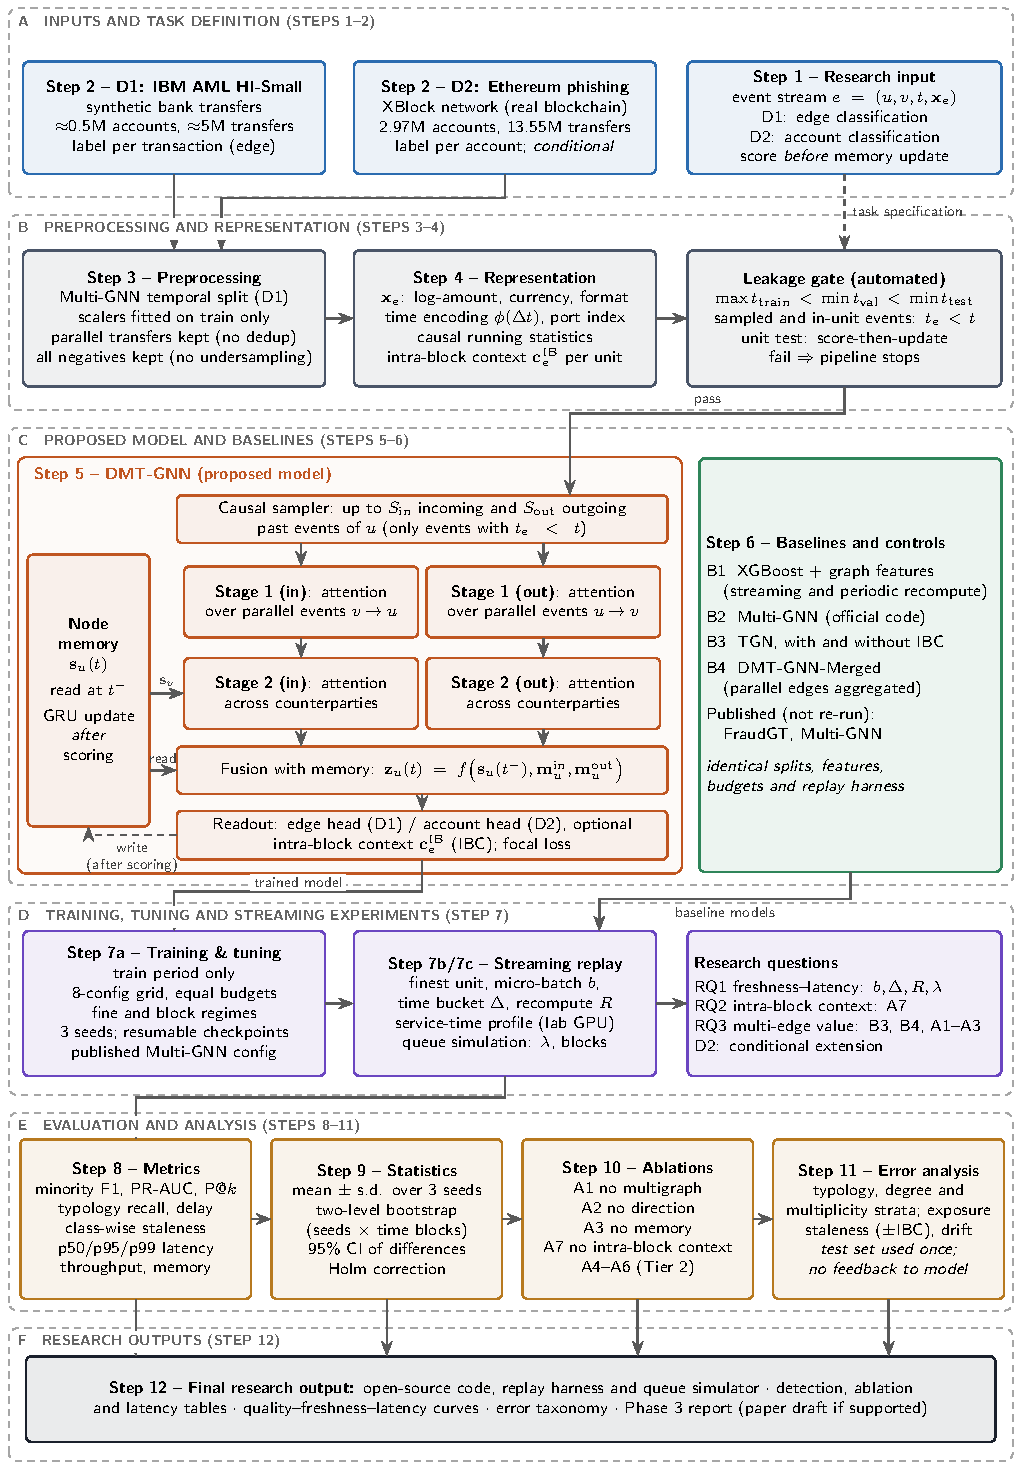
\includegraphics[width=0.98\textwidth,height=0.78\textheight,keepaspectratio]{methodology_architecture.pdf}
    \caption{Research methodology architecture of the proposed DMT-GNN study. The twelve steps are organised in six bands: (A) inputs and task definition (Steps 1--2), (B) preprocessing and representation (Steps 3--4), (C) proposed model and baselines (Steps 5--6), (D) training, tuning and streaming experiments (Step 7), (E) evaluation and analysis (Steps 8--11), and (F) research outputs (Step 12). Dashed arrows denote the task specification and the memory write that occurs only after scoring.}
    \label{fig:methodology_architecture}
\end{figure}

\subsection{Architectural Narrative and Operational Band Dynamics}
\begin{enumerate}[leftmargin=*]
    \item \textbf{Band A (Steps 1--2):} D1 (IBM AML HI-Small, edge labels; core) and D2 (XBlock Ethereum, account labels; conditional) are represented as event streams $e=(u,v,t,\mathbf{x}_e)$ processed in update units under the score-before-update rule.
    \item \textbf{Band B (Steps 3--4):} Multi-GNN's chronological split, train-only scaling, no de-duplication and no undersampling; event features (log amounts, currency, payment format, port index), time encoding, direction flag, causal running statistics and the intra-block context. The automated leakage gate stops the pipeline if any temporal assertion fails.
    \item \textbf{Band C (Steps 5--6):} the causal sampler feeds Stage 1 (parallel transfers per counterparty) and Stage 2 (across counterparties), separately for incoming and outgoing events; the result is fused with node memory and passed, optionally with the intra-block context, to the edge or account head. The memory is read before scoring and written only afterwards. Baselines B1--B4 run on the same data and harness; FraudGT and Multi-GNN results are published references.
    \item \textbf{Band D (Step 7):} tuning (equal 8-configuration grids for DMT-GNN and TGN; published configuration for Multi-GNN; three seeds; fine and block regimes), inference-only streaming replay across update granularities ($b$, $\Delta$) and periodic recomputation ($R$), and the service-time profile and queue simulation for offered load ($\lambda$) and block arrivals, mapped to RQ1--RQ3.
    \item \textbf{Band E (Steps 8--11):} detection, timeliness, staleness and systems metrics; two-level paired bootstrap with Holm correction; core ablations A1--A3 and A7; error analysis by typology, degree, multiplicity, staleness and drift. The test set is used once, with no feedback into modelling.
    \item \textbf{Band F (Step 12):} code, harness and queue simulator, tables and trade-off curves, error analysis, the Phase 3 report and, if supported by the results, a paper draft.
\end{enumerate}

% =========================================================================
% Project Execution Plan, Feasibility, and Risk Management
% =========================================================================
\section{Project Execution Plan, Feasibility, and Risk Management}
\label{sec:execution_plan}

\subsection{Phase 3 Implementation Plan (21 Days)}
The original plan assumed twelve weeks and continuous access to one GPU. Phase 3 has 21 days (26 October -- 15 November 2026), and the lab GPU is available for only 2--3 hours per day, without guaranteed overnight or uninterrupted use. The plan is therefore built around three rules: (i) everything that depends only on the data is computed once on CPU and reused; (ii) every GPU job is short or resumable; and (iii) long unattended GPU jobs run on free Kaggle notebooks, while the lab GPU is reserved for work that needs the target hardware. Table~\ref{tab:phase3_plan} lists the milestones and decision gates; a detailed day-by-day plan is kept in the project repository.

\begin{table}[htbp]
\centering
\scriptsize
\caption{Phase 3 Milestones and Decision Gates (2026)}
\label{tab:phase3_plan}
\begin{tabularx}{\textwidth}{L{0.8cm} L{1.4cm} X L{2.0cm} L{3.0cm}}
\toprule
\textbf{ID} & \textbf{Dates} & \textbf{Work} & \textbf{Machine} & \textbf{Exit criterion} \\
\midrule
M0 & 26--27 Oct & Lab environment (user-level Python, PyTorch, PyG); Kaggle notebook with the IBM dataset attached; data download; Multi-GNN formatter; dataset card & Lab (1 session), Mac, Kaggle & Environment check passes; card matches published counts \\
\midrule
M1 & 26--29 Oct & CPU precomputation: sorted stream, causal features, neighbour indices and IBC per granularity, merged aggregates, exposure $\rho_g$ by class and typology; B1 (continuous mode) & Mac, HP & First B1 result; Gate G0 decided \\
\midrule
G0 & 28 Oct & Exposure diagnostic against criteria fixed in advance (Section~\ref{sec:compute_strategy}) & --- & Keep or reduce RQ2 \\
\midrule
M2 & 27--31 Oct & TGN edge classifier, resumable runner, leakage tests; DMT-GNN and IBC tested on a 1\% subset; timing of one full epoch per model & Lab (2 sessions), Mac & Tests pass; measured epoch times \\
\midrule
G1 & 30 Oct & Fix the run matrix, machine per job, precision and run packing from the measured times & --- & Table~\ref{tab:compute_budget} filled with measurements \\
\midrule
M3 & 28 Oct -- 7 Nov & Tuning grids; fine-regime runs (TGN, DMT-GNN, B4, A2, A3; 3 seeds); Multi-GNN (2 seeds) & Kaggle (unattended), Lab & Checkpoints and validation scores logged \\
\midrule
M4 & 2--8 Nov & Block-regime runs with and without IBC (DMT-GNN, TGN); service-time profiles; streaming sweeps; queue simulation & Lab (sessions), Mac & Score files for all granularities; latency curves \\
\midrule
G2 & 5 Nov & Are at least 80\% of core runs finished and evaluated? & --- & Extension (LI-Small or D2 window, 1 seed) or drop \\
\midrule
M5 & 8--11 Nov & Statistics, stratified and per-typology analysis, figures; live validation of the queue simulation & Mac, HP, Lab (1 session) & All tables and figures generated from logs \\
\midrule
M6 & 9--13 Nov & Phase 3 report (drafting from 27 Oct), code release, demonstration (optional) & All & Report complete; freeze on 13 Nov \\
\midrule
Buffer & 14--15 Nov & Proofreading and submission & --- & Submitted \\
\bottomrule
\end{tabularx}
\end{table}

\subsection{Compute Strategy Under Limited GPU Access}
\label{sec:compute_strategy}
\paragraph{Available resources.} The lab PC (RTX 4000 Ada, 20\,GB, BF16-capable; Intel i7-14700; 32\,GB RAM) is planned at 2--3\,h on about 14 weekdays, i.e.\ 28--42 interruptible GPU hours. Kaggle's free tier is commonly reported to offer about 30 GPU hours per week per account with sessions of up to 12\,h that run in the background; these figures are unofficial and must be confirmed in the team's accounts, so we plan with 40--60 usable hours. The MacBook Pro (M1 Pro, 32\,GB) and the HP laptop (i5-1235U, 20\,GB) run CPU work, including overnight. The lab GPU is used for pilot timing, service-time profiling, the live validation run, short resumable runs and inference sweeps; Kaggle is used for full training runs and the Linux-only Multi-GNN code. Accuracy results do not depend on the device; all latency and throughput results come from the lab GPU only.

\paragraph{Techniques that are worthwhile for this workload.} The models are small (hidden size $\le128$), the training stream is processed sequentially because memory carries state between units, and per-step work is small, so GPU time is dominated by kernel-launch and data-preparation overheads rather than arithmetic. The following therefore matter most:
\begin{enumerate}[leftmargin=*]
    \item \textit{CPU precomputation of everything data-dependent:} the sorted event stream, the most recent $S$ neighbour indices of each event for each update granularity, causal statistics, intra-block context, merged-edge aggregates and the exposure statistic are computed once on the laptops, with an in-process columnar engine (DuckDB or polars), stored as Parquet files and reused by every model and seed. This also removes the dependence on Kaggle's weak CPUs.
    \item \textit{Data resident on the GPU:} the event stream and index tables (a few GB) stay in GPU memory, so no host--device copies occur per step.
    \item \textit{Checkpoint and resume:} every run checkpoints model, optimiser, memory, neighbour buffers, random-number states and stream position at least every 10 minutes (atomic write), and stops cleanly before a time budget expires; a job queue resumes it in the next session or on another machine.
    \item \textit{Automated evaluation off the GPU:} GPU jobs write per-transfer score files; a watcher script on a laptop computes all metrics, bootstrap intervals and figures.
    \item \textit{Cheap tuning:} a small grid on 25\% of the training period with successive halving (the worse half of configurations is stopped after one epoch).
    \item \textit{Block training and inference-only sweeps:} block-regime training needs far fewer sequential steps, and all granularity sweeps reuse trained checkpoints; only the finest-granularity replay is expensive, and it is run once per checkpoint.
    \item \textit{Queue simulation:} measured service times plus a discrete-event simulation replace long live load tests.
\end{enumerate}
\paragraph{Techniques adopted only if the pilot shows a gain.} Running two to four independent runs concurrently on the 20\,GB GPU to fill idle gaps (kept only if aggregate events per second improve by at least 1.3$\times$); BF16 autocast for attention and MLP layers, with the GRU memory and the loss kept in FP32 (the expected gain is small for models this size); TF32 matrix multiplication, which costs nothing to enable.
\paragraph{Techniques not used.} \texttt{torch.compile} and CUDA graphs (limited Windows support, compile time that consumes short sessions, and variable unit sizes that trigger recompilation); multi-GPU training; large Bayesian hyperparameter searches; reduced precision for the recurrent memory.

\paragraph{Hosted notebooks: molab.} molab, the hosted notebook service of the marimo project, provides free notebooks with 4 CPUs and 32\,GB of RAM and, as a public preview, an optional NVIDIA RTX Pro 6000 Blackwell GPU with 96\,GB of memory; a notebook runs for at most 12\,h and is shut down after more than 90 minutes of inactivity.\footnote{\url{https://docs.marimo.io/guides/molab/}, accessed 25 October 2026.} Its GPU far exceeds what our models need, so its value lies in \emph{availability} and in offering a consistent GPU model, which makes it a suitable fallback for latency profiling if the lab PC is unavailable. Three properties limit it: the documentation does not define inactivity, so it is unknown whether a running job survives with the browser closed; persistent storage is small, so derived files are rebuilt from the raw data at the start of a session; and notebooks are public by default, so no credentials may appear in notebook code. We therefore adopt molab as an additional GPU resource only after three acceptance tests (GPU attachment, survival of a two-hour job with the browser closed, and data-loading time). Until it passes them, Kaggle, whose committed runs continue after the browser is closed, remains the primary resource for unattended training, and Google Colab serves only as attended overflow.

\paragraph{Gate G0 (exposure diagnostic).} Before any model is trained, the exposure statistic $\rho_g$ (Step 8) is computed at $\Delta=10$\,min. The criteria are fixed in advance: RQ2 is kept as planned if the mean exposure of illicit transfers is at least 0.10 \emph{or} at least 1.5 times that of benign transfers; otherwise RQ2 is reduced to one exploratory configuration, and RQ1 is reported as measured (a flat staleness curve is also a finding).

\paragraph{Reference points for the budget.} The only published cost figures for comparable models on D1 are those of Egressy et al.\ \cite{egressy2024multigraph}: on an NVIDIA RTX 3090, a full training run took 1,876\,s for plain GIN and 12,958\,s ($\approx$3.6\,h) for GIN with reverse message passing, ports and ego IDs, with inference throughput between 18,700 and 58,663 transactions per second. Training times for memory-based models on HI-Small are not reported in the sources examined, so the ranges in Table~\ref{tab:compute_budget} are planning assumptions until Gate G1.

\begin{table}[htbp]
\centering
\small
\caption{Planned GPU Compute for Phase 3 (planning ranges; replaced by measurements at Gate G1)}
\label{tab:compute_budget}
\begin{tabularx}{\textwidth}{L{4.4cm} L{4.0cm} L{1.4cm} c X}
\toprule
\textbf{Task} & \textbf{Runs} & \textbf{Where} & \textbf{h/run} & \textbf{GPU h} \\
\midrule
Pilot timing & one epoch per model & Lab & --- & 1--2 \\
Tuning grids (TGN, DMT-GNN) & $2\times8$ configurations, 25\% window & Kaggle, Lab & 0.1--0.4 & 2--6 \\
Fine-regime runs (TGN, DMT-GNN, B4, A2, A3) & $5\times3$ seeds & Kaggle & 0.7--2.5 & 11--38 \\
Block-regime runs $\pm$ IBC (DMT-GNN, TGN) & $4\times3$ seeds & Lab & 0.2--0.6 & 2.5--7 \\
Multi-GNN (B2) & 1 configuration $\times$ 2 seeds & Kaggle & 4--8 & 8--16 \\
Streaming sweeps (inference only) & 18 checkpoints $\times$ 7 granularities; 9 $\times$ 2 & Lab, Kaggle & --- & 8--12 \\
Service-time profiles, live validation & 4 models & Lab & --- & 1.5--2 \\
B1, features, evaluation, simulation & --- & CPU & --- & 0 \\
\midrule
\textbf{Total} & & & & \textbf{34--83} \\
\bottomrule
\end{tabularx}
\end{table}

\paragraph{Feasibility assessment.} Planned capacity is 68--102 GPU hours (28--42 on the lab PC and 40--60 on Kaggle), against a requirement of 34--83 hours. The lower end fits easily; the upper end needs both resources near their planned values. If Gate G1 projects more than the available capacity, reductions are applied in this order: (1) A2 with 2 seeds and ablation sweeps at two granularities only; (2) fine-regime units of 500 instead of 200 events (reported as part of the freshness analysis); (3) Multi-GNN with 1 seed, or its published values only; (4) A2 dropped, leaving A1, A3 and A7 as the three core ablations. LI-Small and D2 are attempted only after Gate G2. These are planning estimates, not measurements.

\paragraph{Memory footprint.} With memory and hidden size 128 (FP32), node memory needs about $0.5\text{M}\times128\times4\,\text{B}\approx256$\,MB on D1 and $2.97\text{M}\times128\times4\,\text{B}\approx1.5$\,GB on D2. A unit of 4,000 events with $S_{\text{in}}+S_{\text{out}}=20$ sampled events of width 128 needs about $4{,}000\times20\times128\times4\,\text{B}\approx41$\,MB of activations per layer, and the precomputed neighbour indices for D1 need about $5\text{M}\times20\times4\,\text{B}\approx0.4$\,GB per granularity. All fit in 20\,GB of GPU memory and leave room for concurrent runs.

\subsection{Risk Assessment and Mitigation Strategies}
Table~\ref{tab:risk_management} lists the main technical and scientific risks.

\begin{table}[htbp]
\centering
\small
\caption{Risk Assessment and Mitigation Strategy Matrix}
\label{tab:risk_management}
\begin{tabularx}{\textwidth}{L{2.6cm} L{3.4cm} L{1.4cm} X}
\toprule
\textbf{Identified Risk} & \textbf{Operational Impact} & \textbf{Level} & \textbf{Mitigation Strategy} \\
\midrule
\textbf{R1: No accuracy gain} & DMT-GNN matches but does not beat B3/B4; IBC recovers little. & Moderate & RQ3 and RQ2 are questions, not promises: well-controlled negative results, together with the streaming trade-off curves (RQ1), are still a contribution. \\
\midrule
\textbf{R2: Compute overrun} & Runs exceed the 34--83\,h plan. & High & Gate G1 with measured times; the ordered reduction list (Section~\ref{sec:compute_strategy}); inference-only sweeps; extensions only after Gate G2. \\
\midrule
\textbf{R3: Multi-GNN not reproducible in time} & Missing main multigraph baseline. & Moderate & 5-day time box on Linux (Kaggle); otherwise report published numbers as non-reproduced references; never present a re-implementation as Multi-GNN. \\
\midrule
\textbf{R4: Lab PC access} & Sessions shorter than planned, interrupted, or no installation rights. & High & Resumable runs with 10-minute checkpoints; all long training on Kaggle; if the lab PC cannot be used at all, profiling moves to the Kaggle GPU and the device is stated. \\
\midrule
\textbf{R5: Kaggle quota} & Fewer free GPU hours or shorter sessions than assumed. & Moderate & Confirm quotas in the first week of Phase 3; each team member uses their own account; apply the reduction list. \\
\midrule
\textbf{R6: Novelty overlap} & A 2026 paper already reports AML freshness curves or an equivalent mitigation. & Moderate & Read AnchorRM and StreamTGN in full in the first week of Phase 3; repeat the literature search before any submission; frame IBC as a simple mitigation, not a new architecture. \\
\midrule
\textbf{R7: Negative exposure diagnostic} & Illicit transfers are not more exposed to intra-unit staleness. & Moderate & Gate G0 reduces RQ2 to an exploratory run; RQ1 is still measured and reported. \\
\midrule
\textbf{R8: Leakage bugs} & Inflated results. & Moderate & Automated temporal assertions and the score-then-update unit test in every run. \\
\midrule
\textbf{R9: Label noise in D2} & Unlabelled phishing accounts counted as negatives depress precision. & Moderate & Report P@$k$ and PR-AUC; sensitivity analysis excluding very low-activity accounts; state the assumption explicitly. \\
\midrule
\textbf{R10: Coarse timestamps} & Fine time buckets cannot be distinguished; equal-timestamp events have an arbitrary order. & Low & Check resolution on download; equal-timestamp events form one unit and never see each other; collapse buckets to the available resolution and report this. \\
\midrule
\textbf{R11: Queue saturation at high $\lambda$} & Unbounded latency. & Low & This is a measured outcome: the largest $\lambda$ with a bounded queue defines the sustainable throughput. \\
\bottomrule
\end{tabularx}
\end{table}

% =========================================================================
% Publication Potential
% =========================================================================
\section{Publication Potential}
\label{sec:publication_potential}

\subsection{Novelty and Scientific Contribution Assessment}
Publication is plausible but not assured, and the recent literature narrows what can be claimed. The contribution is \emph{incremental} on the modelling side and potentially more distinctive on the evaluation side:
\begin{enumerate}[leftmargin=*]
    \item \textbf{Networking and systems (primary):} among the works examined, none measures how the detection quality by class, detection delay, latency and throughput of AML detectors depend on update granularity and offered load. Batch staleness itself is known \cite{su2024pres,zhou2025badgnn,anchorrm2026,streamtgn2026}; the potentially new element is its measured effect on AML outcomes, in particular whether it falls disproportionately on illicit transfers and on specific typologies. This is a hypothesis to be tested, not a finding.
    \item \textbf{Mitigation:} the intra-block context is deliberately simple. Its value as a contribution depends on two things that are not yet known: how much of the staleness penalty it recovers relative to the per-event reference, and whether learned intra-batch reconstruction \cite{anchorrm2026} already covers it. It should be presented as a cheap, strong baseline for this setting rather than as a new architecture.
    \item \textbf{Modelling (secondary):} two-stage, direction-specific multi-edge aggregation already exists offline \cite{bilgi2026mega,ding2024diam,egressy2024multigraph}, and degree-aware aggregation is addressed by SALT-GNN \cite{losavio2026saltgnn}. Our addition is to test it inside continuous-time memory against controlled alternatives (B3, B4, A1--A3). Reviewers will judge this mainly on the size and robustness of the measured effect; offline accuracy is not expected to reach FraudGT's 76.41\% \cite{lin2024fraudgt}.
    \item \textbf{Evaluation:} Multi-GNN's chronological protocol, full imbalance and paired block-bootstrap intervals improve comparability; this is good practice rather than a novelty in itself.
\end{enumerate}

\paragraph{Minimum evidence for a credible submission.} (i) B1 and B2 reproduced close to their published D1 values; (ii) staleness curves with confidence intervals for at least two model families (memory-based and feature-based), with the class-conditional and per-typology breakdown; (iii) latency and sustainable throughput from validated measurements; (iv) the IBC recovered fraction with confidence intervals; (v) DMT-GNN versus B3/B4 with stratified analysis; (vi) a second dataset (LI-Small or D2) for external validity; and (vii) released code. Items (i)--(v) are planned for Phase 3; item (vi) is conditional, which is the main reason a main-track submission is unlikely before further work.

\subsection{Target Publication Venues}
Venue choice depends on the results. Calls for papers and deadlines have not yet been checked.
\begin{itemize}[leftmargin=*]
    \item \textbf{Best scope fit:} the ACM International Conference on AI in Finance (ICAIF), where GFP \cite{blanusa2024gfp} and FraudGT \cite{lin2024fraudgt} appeared, and workshops on anomaly detection or machine learning in finance co-located with KDD or ICDM (Amatriciana is listed as an ICDM 2024 workshop paper \cite{digennaro2025amatriciana}).
    \item \textbf{Blockchain-focused venues:} IEEE conferences on blockchain and cryptocurrency, if the Ethereum results are strong.
    \item \textbf{Networking venues} (e.g., security or blockchain symposia at IEEE ICC/GLOBECOM): only if the streaming-systems results dominate the paper.
    \item \textbf{Main tracks of top AI/data-mining venues} (e.g., AAAI, CIKM, KDD): realistic only with a clear, statistically robust improvement over strong baselines on both datasets, or with a measurement study whose findings generalise across datasets and model families. Neither can be assumed from the Phase 3 scope.
\end{itemize}
Before any submission, the literature search of Section~\ref{sec:selection} is repeated for 2026 work on streaming AML evaluation, and AnchorRM and StreamTGN are read in full.

% =========================================================================
% Conclusion
% =========================================================================
\section{Conclusion}
\label{sec:conclusion}

This Phase 2 document extends the Phase 1 review with nine verified 2025--2026 studies from Q1/Q2 journals and CORE A* conferences, positions the project against the closest earlier work, and turns the resulting gaps into a twelve-step methodology.

The synthesis shows three recurring limitations: (1) parallel transfers between the same accounts are summed, de-duplicated or aggregated before learning; (2) learned detectors are trained and evaluated in batch or snapshot mode, with no measurement of how detection quality depends on update freshness or how latency behaves under load; and (3) random splits, undocumented protocols and balanced re-sampling hinder comparison. Earlier work already handles directed multigraphs offline, streams hand-crafted features, and studies batch staleness for generic temporal graphs, so our refined gap is narrower: what the quality--freshness--latency trade-off of streaming AML detectors is, whether it penalises illicit transfers disproportionately, whether a cheap intra-block context recovers the loss, and whether per-transfer, direction-aware aggregation adds value inside a continuous-time memory model.

The streaming harness, the intra-block context, DMT-GNN and the controlled baselines are designed to answer RQ1--RQ3 on the IBM synthetic bank benchmark under Multi-GNN's chronological, full-imbalance protocol, with the real Ethereum network as a conditional extension. The streaming evaluation, which treats detection as a networked service with block-based delivery, arrival processes, queueing and latency, is the project's main Computer Networks contribution. Revision 2 fits this design into a 21-day Phase 3 with 2--3 lab-GPU hours per day by precomputing data-dependent work on CPU, making every GPU job resumable, and running long jobs on free cloud notebooks; the compute plan will be confirmed by measured pilot times before the main experiments.

% =========================================================================
% Appendices
% =========================================================================
\appendix

\section{Requirement Traceability Matrix}
\label{app:traceability}

Table~\ref{tab:traceability_matrix} maps each Phase 2 requirement to where it is addressed.

\begin{table}[htbp]
\centering
\scriptsize
\caption{Phase 2 Requirement Traceability Matrix}
\label{tab:traceability_matrix}
\begin{tabularx}{\textwidth}{L{4.6cm} X L{3.6cm}}
\toprule
\textbf{Requirement} & \textbf{How it is addressed} & \textbf{Location} \\
\midrule
8--10 additional papers, 2025--2026 & Nine papers; Phase 1 papers excluded; years verified on Crossref & Section~\ref{sec:selection}, Table~\ref{tab:eligibility_audit} \\
Genuine research articles in Q1/Q2 or ranked venues & Seven journal articles (Q1/Q2) and two CORE A* conference papers; sources in Appendix~\ref{app:verification} & Table~\ref{tab:eligibility_audit} \\
Relevance, methodology, data and evaluation & Fifteen headings (A--O) per paper & Section~\ref{sec:individual_analyses} \\
Screening transparency & Excluded candidates with reasons & Table~\ref{tab:excluded} \\
Cross-paper comparison table (title, year, dataset, preprocessing, models, metrics, results, limitations) & Landscape table with split protocol stated; capability matrix & Tables~\ref{tab:cross_paper_comparison}, \ref{tab:capability_matrix} \\
At least three research gaps with evidence from three papers & Four gaps (G4 deferred), evidence from KAR, LMAE4Eth, TAML & Table~\ref{tab:gap_synthesis}, Section~\ref{sec:gap_justification} \\
Refined gap answering six questions & Six questions; gap statement, problem, aim, objectives, RQ1--RQ3 & Section~\ref{sec:refined_gap} \\
Twelve-step methodology & Steps 1--12 with objective, input, procedure, output, justification, literature, risks & Section~\ref{sec:methodology}, Table~\ref{tab:methodology_summary} \\
Methodology architecture diagram & Vector TikZ figure consistent with Steps 1--12 & Figure~\ref{fig:methodology_architecture} \\
Feasibility within the project timeline & Revision 2: 21-day Phase 3 plan with gates G0--G2; compute strategy for 2--3 lab-GPU hours per day; compute budget; risks & Section~\ref{sec:execution_plan}, Tables~\ref{tab:phase3_plan}, \ref{tab:compute_budget}, \ref{tab:risk_management} \\
Publication potential & Contribution assessment and venue fit & Section~\ref{sec:publication_potential} \\
Closest prior work & Multi-GNN, DIAM, MEGA-GNN, GFP, FraudGT (with reported results), SALT-GNN, PRES, BADGNN, AnchorRM, StreamTGN, TeMP-TraG, Amatriciana & Section~\ref{sec:prior_work}, Table~\ref{tab:prior_work_positioning} \\
\bottomrule
\end{tabularx}
\end{table}

\section{Literature Verification Log}
\label{app:verification}

Bibliographic metadata were checked against Crossref (\texttt{api.crossref.org}) and the publisher landing pages in October 2026. Conference ranks were checked on the ICORE portal. The SCImago portal blocked automated access, so journal quartiles come from publisher bibliometric pages or secondary SJR/JCR listings and should be re-confirmed on \url{https://www.scimagojr.com} before final submission. The entries added in Revision 2 (below the FraudGT row) come from arXiv abstract pages and, for StreamTGN, search-result excerpts; their full texts are still to be read, and none of them is counted towards the nine-paper quota.

\begin{table}[htbp]
\centering
\scriptsize
\caption{Literature Verification Log}
\label{tab:verification_log}
\begin{tabularx}{\textwidth}{L{1.7cm} L{2.9cm} L{2.6cm} L{2.3cm} X}
\toprule
\textbf{Key} & \textbf{First author, year, venue} & \textbf{DOI / identifier} & \textbf{Ranking (source)} & \textbf{Full text examined; notes} \\
\midrule
\texttt{yang2025} & X.~Yang, 2025, AAAI-25 & \nolinkurl{10.1609/aaai.v39i20.35508} & CORE2023 A* (ICORE) & arXiv:2412.16447; hyperparameters not reported, so omitted. \\
\texttt{tian2025} & Z.~Tian, 2025, Electronics & \nolinkurl{10.3390/electronics14173345} & SJR Q2 (secondary) & MDPI HTML; result-table values not extracted, so only text-stated results are quoted. \\
\texttt{ferretti2025} & S.~Ferretti, 2025, IEEE Access & \nolinkurl{10.1109/ACCESS.2025.3552240} & SJR Q1 (secondary); SJR 2024 0.849 (IEEE) & IEEE Xplore HTML; split protocol not described. \\
\texttt{li2025} & M.~Li, 2025, Sci.\ Rep. & \nolinkurl{10.1038/s41598-025-08365-9} & JCR Q1 (secondary) & Nature HTML and tables; split not described; baselines borrowed. \\
\texttt{kasula2025} & V.~K.~Kasula, 2025, Discover AI & \nolinkurl{10.1007/s44163-025-00508-1} & SJR Q1, 0.876 (secondary) & Springer HTML and tables. \\
\texttt{jia2025} & Y.~Jia, 2025, IEEE TIFS & \nolinkurl{10.1109/TIFS.2025.3612149} & SJR Q1 (secondary) & Authors' version arXiv:2509.03939v1; may differ slightly from the version of record. \\
\texttt{lin2026} & Z.~Lin, 2026, Sci.\ Rep. & \nolinkurl{10.1038/s41598-025-23901-3} & JCR Q1 (secondary) & Nature HTML; dataset statistics differ from canonical Elliptic. \\
\texttt{alemari2026} & S.~Al-E'mari, 2026, Future Internet & \nolinkurl{10.3390/fi18090461} & SJR Q2 (secondary) & MDPI HTML and tables; adjusted $p=0.074$ (Table~12 of the paper). \\
\texttt{rico2026} & R.~Rico, 2026, IJCAI-26 & \nolinkurl{10.24963/ijcai.2026/723} & CORE2023 A* (ICORE) & Proceedings PDF. \\
\midrule
\texttt{egressy2024} & B.~Egressy, 2024, AAAI-24 & \nolinkurl{10.1609/aaai.v38i10.29069} & CORE2023 A* (ICORE) & arXiv v3 tables and appendix (F1 values, training times, throughput). \\
\texttt{ding2024} & Z.~Ding, 2024, CIKM-24 & \nolinkurl{10.1145/3627673.3679707} & CORE2023 A (ICORE) & Abstract and arXiv record only. \\
\texttt{bilgi2026} & H.~\c{C}.~Bilgi, 2026, TMLR & arXiv:2412.00241v3 & Not verified & Acceptance as stated on arXiv; abstract only. \\
\texttt{blanusa2024} & J.~Blanu\v{s}a, 2024, ICAIF-24 & \nolinkurl{10.1145/3677052.3698674} & Not checked & Abstract only. \\
\texttt{lin2024} & J.~Lin, 2024, ICAIF-24 & \nolinkurl{10.1145/3677052.3698648} & Not checked & Revision 2: author PDF, Tables 1--2 (dataset statistics, split, minority F1). \\
\texttt{losavio2026} & L.~Losavio, 2026, arXiv & arXiv:2607.10131v1 & Preprint & Abstract page only (July 2026); code not yet released. \\
\texttt{su2024} & J.~Su, 2024, ICLR-24 & arXiv:2402.04284 & Not checked & Abstract only. \\
\texttt{zhou2025b} & Y.~Zhou, 2025, arXiv & arXiv:2506.19282v1 & Preprint & Abstract only; training-focused. \\
\texttt{anchorrm} & H.~Gharwi, 2026, arXiv & arXiv:2610.27558v1 & Preprint & arXiv abstract (20 Oct 2026); full text still to be checked. \\
\texttt{streamtgn} & L.~Zhang, 2026, arXiv & arXiv:2603.21090v1 & Preprint & arXiv abstract (22 Mar 2026) and search excerpts; full text still to be checked. \\
\midrule
\texttt{chen2025} & S.~Chen, 2025, Adv.\ Intell.\ Syst. & \nolinkurl{10.1002/aisy.202400898} & Q1 (secondary) & Excluded: full text behind a bot-verification page; abstract only. \\
\texttt{zhou2025} & W.-G.~Zhou, 2025, IEEE Access & \nolinkurl{10.1109/ACCESS.2025.3553377} & Q1 (secondary) & Excluded: non-financial datasets. \\
\texttt{asiri2025} & A.~Asiri, 2025, Sci.\ Rep. & \nolinkurl{10.1038/s41598-025-95672-w} & JCR Q1 (secondary) & Excluded: anomalies confirmed in the PubMed Central full text. \\
\bottomrule
\end{tabularx}
\end{table}

\bibliographystyle{IEEEtran}
\bibliography{references}

\end{document}
